\documentclass[11pt]{article}
\usepackage[T1]{fontenc}
\usepackage[utf8]{inputenc}
\usepackage{lmodern,amsmath,amssymb,amsthm,mathtools,booktabs,enumitem,microtype,longtable,array,tikz}
\input{glyphtounicode-cmex}
\pdfgentounicode=1
\usepackage[margin=1in]{geometry}
\usepackage[colorlinks=true,linkcolor=blue,urlcolor=blue,citecolor=blue]{hyperref}
\hypersetup{pdftitle={Prefix Instructions and Incompressible Flows},pdfauthor={OpenAI}}
\newtheorem{theorem}{Theorem}[section]
\newtheorem{lemma}[theorem]{Lemma}
\newtheorem{corollary}[theorem]{Corollary}
\newtheorem{proposition}[theorem]{Proposition}
\newtheorem{definition}[theorem]{Definition}
\theoremstyle{remark}
\newtheorem{remark}[theorem]{Remark}
\newcommand{\T}{\mathbb T}
\newcommand{\Z}{\mathbb Z}
\newcommand{\N}{\mathbb N}
\newcommand{\R}{\mathbb R}
\newcommand{\Q}{\mathbb Q}
\newcommand{\diag}{\operatorname{diag}}
\newcommand{\supp}{\operatorname{supp}}
\newcommand{\divg}{\operatorname{div}}
\newcommand{\id}{\operatorname{id}}
\title{Prefix Instructions and Incompressible Flows}
\author{OpenAI}
\date{September 27, 2026}
\begin{document}
\maketitle
\begin{abstract}
Finite prefix instructions may change area and erase information. We give
explicit history processors and smooth incompressible motions that retain
that information and realize every instruction on its full domain. A first
application assigns each machine and finite input a smooth mean-zero force
on the flat unit three-torus, at any fixed positive computable viscosity.
The solution starts from rest; a fixed particle enters a fixed open strip
exactly when the machine halts. The force repeats with period one after an
initial loading interval. We then prove alternative realizations using
full boxes, normal compensation, invariant planes, and a spatial clock.
The constructions specify their initialization, comparison class, derivative
bounds, and continuous-time observation. Exact formulas and effective
cutoffs provide finite descriptions of the fields and all their derivatives.
\end{abstract}
\section{Introduction}
A finite machine instruction reads a short part of a configuration and
changes it. A material flow, by contrast, must be invertible at every
finite time. Two questions therefore arise when a particle is to carry a
computation: where is the information erased by an instruction retained,
and how is the resulting injective update made compatible with
incompressibility? We study these questions for finite prefix instructions
and their smooth three-dimensional realizations.

A stack is an infinite word whose first letter is its accessible end.
A prefix instruction has the form
\[
 (s;v,w)\longmapsto(s';v',w'),
\]
meaning that it sends $(s,vL,wR)$ to $(s',v'L,w'R)$ for every pair of
unchanged tails $L,R$. Here $s,s'$ belong to a finite set of control
states, and all four prefixes are finite words over a finite alphabet.
A positional code turns this operation into a positive diagonal affine
map between two rectangles. The source rectangles must be separately
disjoint, and so must the target rectangles. Intersections between a
source rectangle and a target rectangle are allowed. These conditions
are stronger than injectivity along one initialized computation.

The planar map need not preserve area. Appending one history letter,
for example, contracts one stack coordinate without expanding the
other. We realize such instructions in two ways. A compensating normal
strain transports the entire coded rectangle and a three-dimensional
neighborhood. Alternatively, a compressible planar motion is placed in
an invariant plane of an incompressible field. The latter preserves the
prescribed planar dynamics without prescribing an affine map off the
plane. Both methods require control of the complete continuous path:
correctness at integer sampling times alone does not establish a fixed
particle observation.

\subsection{The fluid problem and a first result}
Let $\mathbb T^3=(\mathbb R/\mathbb Z)^3$ with its flat metric, and fix a
positive computable viscosity $\nu$. For an arbitrary fixed positive real
$\nu$, the same formulas and conclusions hold, and numerical evaluation
is relative to that coefficient. We use
\begin{equation}\label{eq:sheets-ns}
 u_t+(u\cdot\nabla)u-\nu\Delta u+\nabla p=f,
 \qquad \operatorname{div}u=0,\qquad u(0)=0.
\end{equation}
An instance is a deterministic machine with finite state set, finite work
alphabet with a blank, an initial state, a specified halt set, and a
finite input written on an otherwise blank two-sided tape. Its head
starts at cell zero. Missing transitions may be interpreted as halting.
For a fixed initial label $a$, the material position satisfies
$X'(t)=u(t,X(t))$ and $X(0)=a$. The observation asks whether
$X(t)\in O$ for some $t\ge0$, where $O$ is a fixed open set.

A finite effective force prescription is a finite program that evaluates
$f$ and any requested mixed derivative at computably specified arguments
to any positive rational error, and supplies the derivative bounds used
on compact sets. The program describes every instruction branch. It does
not generate a machine execution and replay that execution as a force.
On a torus our classical comparison class requires $u,u_t$, spatial
derivatives of $u$ through order two, and $p,\nabla p$ to be continuous
on every finite closed time cylinder. Velocity and pressure are periodic,
and pressure has spatial mean zero. The prescribed solutions themselves
are smooth.

\begin{theorem}[Interspersed history on moving sheets]\label{thm:sa-interleaved}
At fixed positive computable viscosity, every machine and finite input
effectively determine a smooth mean-zero general force on the unit
$\mathbb T^3$, with all mixed derivatives bounded and period one for
$t\ge1$.  Its zero-data solution is globally smooth and unique in the
classical periodic comparison class, with uniformly bounded kinetic
energy.  Its material trajectory from $(1/8,1/4,1/4)$ enters
$\{x:1/2<x_1<1\}$ at some finite time exactly when the machine halts.
The repeated template depends only on the table, and the input enters
only the loading pulse.
\end{theorem}


This first result is proved with history records interspersed among work
letters. Its geometric map changes planar area, so a third scale restores
volume. Later constructions change the history arrangement or initialization
when a different property is wanted: compact Euclidean support, a bounded
detector, periodicity from the initial time, or a spatial clock. The
comparison classes, initial labels, detectors and temporal conclusions are
stated separately for these alternatives.

\subsection{Antecedents and the role of the present constructions}
The logical obstruction comes from Turing's undecidable symbol-printing
problem~\cite[Section~8]{Turing1936}. Modify such a machine to halt at
the first printing of the designated symbol, and redirect any earlier
ordinary stop into an infinite dummy loop. It then halts exactly when
the designated symbol would have been printed, giving the halting
formulation used here. Retaining information lost by an irreversible instruction was
discussed by Landauer~\cite[Section~3]{Landauer1961} and implemented by
Bennett's history recording~\cite[Eqs.~(9)--(11)]{Bennett1973}. Our
histories remain stored. We prove the local tables and their inverses
explicitly; the cleanup and complexity statements of Bennett's reversible
simulation are not used.

Moore's generalized shifts connect finite symbolic instructions with
positional codes and piecewise affine dynamics
\cite{Moore1990,Moore1991}. The smooth realization and suspension for
invertible generalized shifts in
\cite[Section~6, Theorem~12 and its corollary]{Moore1991} are direct
antecedents of the present viewpoint. We need additional statements on
full closed rectangles, effective derivative bounds, incompressibility,
zero initial velocity, and observation at every intermediate real time.
These are established by the explicit motions below. The classical
fragility of positional tape storage also explains why an exact event
should not be read as a uniform finite-precision tolerance.

Cardona, Miranda, Peralta-Salas and Presas constructed Turing-complete
stationary Euler particle flows on a three-sphere with a chosen metric
\cite{CardonaMirandaPeraltaSalasPresas2021}. Their area-preserving
extension of generalized shifts uses contraction, transport and expansion
of separated blocks followed by a relative area correction
\cite[Proposition~5.1]{CardonaMirandaPeraltaSalasPresas2021}.
That construction is an important predecessor of the planar routing used
here. Our explicit normal compensation and invariant-plane formulas give
the prescribed flat three-dimensional motions directly; their full
neighborhood and detector properties are proved at the point of use.
Cardona, Miranda and Peralta-Salas also constructed Turing-complete
stationary Euler flows for the standard Euclidean metric on $\R^3$,
with computation on a noncompact invariant plane and infinite kinetic
energy \cite[Theorem~1 and the discussion following it]{CardonaMirandaPeraltaSalas2023Beltrami}.

Universality is also known with viscosity. Dyhr, Gonz\'alez-Prieto, Miranda
and Peralta-Salas construct unforced stationary Navier--Stokes particle
universality on suitable compact three-manifolds after deforming the metric,
using Hodge viscosity and a harmonic velocity
\cite[Theorem~A]{DyhrGonzalezPrietoMirandaPeraltaSalas2026}.
The fixed flat domains, prescribed external force, and zero initial
velocity in the present paper specify a different fluid experiment.
Our results concern these constructed solutions and exact material events;
they make no assertion about arbitrary-data regularity.

The companion \emph{Finite Instructions and Solenoidal Shear Flows}
\cite{OpenAIShear2026} gives a complete initialized construction with
reciprocal planar maps and directly solenoidal force at pressure zero.
We use its full-domain recorder in one later specialization, with an
explicit identification of all guards. The general residual forces below
need not be solenoidal. When a torus force is projected, the accompanying
pressure changes; that operation is kept distinct from the direct shear
identity.

\subsection{Proof strategy and reading order}
The first application has four steps. Gapped radix intervals turn complete
prefix cylinders into separated closed rectangles. A local curl formula
then implements an affine volume-preserving motion on a neighborhood.
Private heights separate the instruction rectangles while a reciprocal
normal strain corrects their planar area changes. Finally, a history
invariant identifies the computation, a loading segment places the fixed
particle at its initial code, and the horizontal interpolation proves
the detector equivalence throughout every instruction period.

Section~\ref{sec:model} records the residual realization and the exact
analytic comparison classes. Section~\ref{sec:sa-sheets} develops the
radix and moving-sheet tools. Section~\ref{sec:sa-histories} completes
Theorem~\ref{thm:sa-interleaved}. Sections~\ref{sec:sheets-boxes}
and~\ref{sec:sheets-planes} then explain the additional requirements of
full boxes and invariant-plane routing. Sections~\ref{sec:sa-separator-histories}--\ref{sec:sa-marked-five-stage}
organize the resulting processors by where they retain history: next to
a separator, on a tape track, or in a separate stack.
Sections~\ref{sec:sb-prefix}--\ref{sec:sb-events} treat further
history placements, boot instructions and fixed observers.
Section~\ref{subsec:p2:rapid-periodic} gives two compact reciprocal
realizations. The final section replaces a temporal program by a spatial
clock and verifies its separate decay and phase-window observation.

\section{Analytic classes and changes of physical coordinates}\label{sec:model}
The geometric constructions prescribe a smooth velocity first. This section
records exactly which other solutions are excluded by the energy argument.
Pressure assumptions are kept separate: continuity in a pressure norm, a
norm at each individual time, and an integrable pressure gradient are
different conditions.

Write $\mathcal F_\nu[U]=U_t+(U\cdot\nabla)U-\nu\Delta U$.
All noncompact results below use $\mathbb R^3$; their velocities and forces
have one fixed compact spatial support unless the individual statement
says otherwise. This property concerns the constructed solution, not a
competing solution. On $[0,T]$, write $CH^k=C([0,T];H^k(\mathbb R^3))$
and $C^1L^2=C^1([0,T];L^2(\mathbb R^3))$. Spatial constants in pressure
may depend on time.

\begin{lemma}[The pressure term without a pressure norm]\label{lem:b-gradient}
If $w,g\in L^2(\mathbb R^3;\mathbb R^3)$ satisfy
$\operatorname{div}w=0$ and $\operatorname{curl}g=0$ in distributions, then
$\langle w,g\rangle_{L^2}=0$. In particular, any distributional gradient
$g=\nabla p\in L^2$ has zero pairing with $w$, without an assumption that
$p\in L^2$.
\end{lemma}
\begin{proof}
An $L^2$ field is a tempered distribution. The differential identities,
initially tested on compactly supported smooth functions, extend to
Schwartz tests by multiplying by cutoffs tending to one and using $L^2$
convergence of the tests and their first derivatives. Fourier transformation
gives $\xi\cdot\widehat w=0$ and
$\xi_j\widehat g_k-\xi_k\widehat g_j=0$. These are identities of locally
integrable functions, so they hold almost everywhere. Away from $\xi=0$,
$\widehat g$ is parallel to $\xi$ and $\widehat w$ is perpendicular to it.
Their Hermitian product is zero. The exceptional point has measure zero;
Plancherel proves the assertion.
\end{proof}

\begin{lemma}[Residual realization and separate comparison classes]
\label{lem:b-comparison}\label{lem:p2-realization}
Let $\nu>0$ and let $U$ be a prescribed smooth divergence-free velocity
on $[0,\infty)\times\mathbb R^3$, with $U(0)=0$. On each finite interval,
assume $U\in CH^2\cap C^1L^2$ and $U,\nabla U$ are bounded. Put
$f=\mathcal F_\nu[U]$. Then $(U,0)$ is a solution. Its velocity is unique
in each of the following separately stated comparison classes, with the
same force and initial data:
\begin{enumerate}[label=(\roman*),itemsep=2pt]
\item Smooth classical $v\in CH^2\cap C^1L^2$, with bounded $v$, and a
pressure representative $p\in CH^1$.
\item Smooth classical $v\in CH^2\cap C^1L^2$, with bounded $v,\nabla v$,
and an $H^1$ pressure representative at each time, with no required time
continuity in that pressure norm.
\item Strong solutions with $v\in CH^4\cap C^1H^2$ and distributional
$\nabla p\in CL^2$.
\item Smooth classical $v\in CH^2\cap C^1L^2$, with bounded $v,\nabla v$,
and a pressure representative $p\in CL^2$.
\item Smooth classical $v\in CH^2\cap C^1L^2$, with bounded $v,\nabla v$,
without an additional integrability or normalization condition on pressure.
\end{enumerate}
The pressure gradient is unique. An $L^2$ pressure representative, when
specified, is zero; otherwise pressure is determined up to a function of
time. The reference material flow is a smooth diffeomorphism at every
finite time and exists for every finite forward time.

On a flat torus $\T_L^3$, the same conclusion holds in the classical class
where $v,v_t$, spatial derivatives through order two, and $p,\nabla p$ are
continuous on finite closed cylinders, with periodic mean-zero pressure.
No Sobolev conditions at infinity are involved in that assertion.
\end{lemma}
\begin{proof}
Substitution proves existence of the prescribed solution. Set $w=v-U$.
The difference equation is
\[
 w_t+(v\cdot\nabla)w+(w\cdot\nabla)U
    =\nu\Delta w-\nabla p,\qquad \operatorname{div}w=0.
\]
The stated velocity regularity implies $w\in C^1L^2\cap CH^2$, so
$\frac d{dt}\|w\|_2^2=2\langle w,w_t\rangle$ at each time. In case
(iii), the stronger assumptions imply these inclusions. They also imply
bounded velocity and spatial derivatives through order two: for $j\le2$,
Cauchy--Schwarz in Fourier space uses the finite integral
$\int_{\mathbb R^3}|\xi|^{2j}(1+|\xi|^2)^{-4}\,d\xi$.

For the transport term, insert a cutoff $\chi_R$ that equals one on the
ball of radius $R$, is supported in the ball of radius $2R$, and satisfies
$|\nabla\chi_R|\le C/R$. Its boundary error is at most
$CR^{-1}\|v\|_\infty\|w\|_2^2$, which tends to zero. Diffusion is
integrated by parts in $H^2$; alternatively its cutoff error is bounded by
$CR^{-1}\|w\|_2\|\nabla w\|_2$. The deformation term is bounded by
$\|\nabla U\|_{\infty,\mathrm{op}}\|w\|_2^2$.

The same pressure cancellation applies in all five classes. At each time,
the equation gives the following equality of distributional gradients in
$L^2$:
\[
 \nabla p=f-v_t-(v\cdot\nabla)v+\nu\Delta v\in L^2,
 \qquad \|(v\cdot\nabla)v\|_2\le\|v\|_\infty\|\nabla v\|_2.
\]
The velocity assumptions in every class give all terms on the right in
$L^2$; the identical estimate for $U$ and its stated time and space
regularity give $f\in L^2$. Since a distributional gradient is curl free,
Lemma~\ref{lem:b-gradient} gives $\langle\nabla p,w\rangle=0$.
This cancellation neither chooses an $L^2$ pressure representative nor
uses continuity of pressure in a norm.

In every case the resulting pointwise energy inequality is
\[
 \frac12\frac d{dt}\|w\|_2^2+\nu\|\nabla w\|_2^2
 \le \|\nabla U\|_{\infty,\mathrm{op}}\|w\|_2^2.
\]
The coefficient is bounded on each finite interval and $w(0)=0$, so an
integrating factor gives $w=0$. The pressure has already disappeared before
time integration; the proof imposes no unlisted temporal pressure norm.
Substitution then gives $\nabla p=0$. A spatially constant $L^2$ function
on $\mathbb R^3$ is zero, which proves the normalization assertion.

On the torus every integration by parts is periodic and has no boundary
term. The specified classical regularity justifies norm differentiation,
diffusion, and pressure cancellation. The same energy inequality gives
uniqueness and the mean-zero normalization fixes pressure. In either domain,
the smooth reference velocity and its bounded spatial derivative give
unique material trajectories; bounded speed prevents finite-time escape.
Solving backwards on a finite interval gives the inverse flow, and smooth
ODE dependence gives its smoothness.
\end{proof}

Cases (i)--(v) identify the precise hypotheses used by the applications;
their presence in a common lemma does not replace a theorem's declared
comparison class by a different one. In particular, a pressure norm is not
silently imposed in a gradient-only application. The proof is the classical
energy comparison for prescribed smooth solutions \cite[Section~18]{Leray1934},
with its noncompact pressure pairings made explicit.

For the flow $\Phi_t$, differentiation of its trajectory equation gives
\[
 U(t)=(\partial_t\Phi_t)\circ\Phi_t^{-1},\qquad
 \partial_{tt}\Phi_t(a)=
 (f-\nabla p+\nu\Delta U)(t,\Phi_t(a)).
\]
These identities describe the material form of the same constructed solution;
they do not add an independent existence claim.

\begin{lemma}[Physical scaling]\label{lem:p2-chart}
For $a,b>0$, $x=x_0+ay$, and $s=bt$, let
$U(t,x)=abV(bt,(x-x_0)/a)$. Then trajectories are transformed by this change
of variables, incompressibility is preserved, and at the prescribed physical
viscosity $\nu$,
\[
 \mathcal F_\nu[U](t,x)=ab^2\left[
 V_s+(V\cdot\nabla_y)V-\frac{\nu}{a^2b}\Delta_yV
 \right](bt,(x-x_0)/a).
\]
\end{lemma}
\begin{proof}
The trajectory equation gives $\dot x=abV$; differentiating in space gives
$\operatorname{div}_xU=b\operatorname{div}_yV$. The three residual terms
scale by $ab^2,ab^2$, and $b/a$, respectively, proving the formula.
\end{proof}
Thus a side-$10$ torus is kept as a physical side-$10$ torus. If a chart
is rescaled, the residual is recomputed with the fixed $\nu$; the equation
is not identified with a differently normalized viscosity.

\begin{proposition}[Projection on a flat torus]\label{prop:projection-l2}
An effective smooth mean-zero force $g$ on $\T_L^3$ has an effective
mean-zero potential $\phi$ satisfying $\Delta\phi=\operatorname{div}g$.
Replacing $(g,p)$ by $(g-\nabla\phi,p-\phi)$ preserves velocity and makes
the force solenoidal. Uniform mixed-derivative bounds, temporal $L^2$
bounds of their spatial suprema, and separately imposed time periodicity,
eventual stationarity, or orderwise decay bounds are preserved.
\end{proposition}
\begin{proof}
In frequencies $\xi_k=2\pi k/L$, set
$\widehat\phi(k)=-i\xi_k\cdot\widehat g(k)/|\xi_k|^2$ for $k\ne0$
and zero for $k=0$. The multiplier from $g$ to $\nabla\phi$ is
$\xi_k\xi_k^{\mathsf T}/|\xi_k|^2$. For a spatial derivative order $r$,
integrate each Fourier coefficient $r+5$ times in a coordinate with largest
$|k_i|$. There are $O(n^2)$ lattice points on the shell $\|k\|_\infty=n$,
so the derivative series and its tail converge absolutely, with
\[
 \|\partial_t^h\partial_x^\alpha\nabla\phi\|_\infty
 \le C_{\alpha,L}\max_i
       \|\partial_t^h\partial_{x_i}^{|\alpha|+5}g\|_\infty.
\]
This bound is pointwise in time, and proves each asserted norm or weighted
time estimate. Derivative bounds give effective Fourier tails; coefficient
integrals can be computed by Riemann sums with derivative error estimates.
The formula gives the Poisson identity, divergence cancellation, and the
pressure sign by substitution. Linearity preserves the time symmetries.
\end{proof}
Projection generally changes pressure. It supplies no compact-support
conclusion on Euclidean space and is distinct from the direct zero-pressure
solenoidal shear construction.

\paragraph{Effective flat profiles.}
For later cutoff formulas put
\begin{equation}\label{eq:p2-step}
 \rho(s)=\begin{cases}e^{-1/s},&s>0,\\0,&s\le0,\end{cases}
 \qquad \sigma(s)=\frac{\rho(s)}{\rho(s)+\rho(1-s)}.
\end{equation}
Positive-side derivatives of $\rho$ are polynomials in $1/s$ times
$e^{-1/s}$ and extend flatly at zero. The estimate
$v^me^{-v}\le(m+k)!v^{-k}$ gives effective error bounds near the seam,
and $\rho(s)+\rho(1-s)\ge e^{-2}$. Products, translations, rescalings,
and derivatives therefore yield effective cutoffs with all requested
derivative bounds. Periodization uses zero collars; at approximate real
arguments a finite superset of possible translates is evaluated. No real
equality test at a seam or execution of the encoded computation is used.

\section{Prefix maps with changing area}\label{sec:sa-sheets}
A stack operation changes a finite prefix and leaves the remaining word
unchanged.  In a positional code this becomes a diagonal affine map of
a rectangle.  The two scale factors need not be reciprocal.  We shall
therefore use either a normal strain to compensate the area change, or
a planar motion embedded in an invariant plane.  These two methods have
different geometric guarantees: the former moves a neighborhood in three
dimensions, whereas the latter preserves one plane throughout the motion.

Throughout these constructions, viscosity is a fixed positive computable
number.  At an arbitrary fixed positive real viscosity, the same formulas
are effective relative to that coefficient: the residual has form
$G+\nu J$ with effective coefficient fields independent of $\nu$.
Coordinate inequalities on the unit torus denote the displayed arcs modulo
one; the path estimates use the stated representatives inside a chart.

\subsection{From prefix cylinders to closed rectangles}\label{subsec:sa-local}
We use the machine convention of a two-sided tape, a finite alphabet with
blank, and moves $-1,0,1$.  A missing instruction interpreted as halting
can be replaced by an instruction that preserves the scanned symbol,
stays in place, and enters a new halt state.  Multiple halt states can
be merged when a construction calls for a single one.  A left-end
convention is represented by a permanent tag at the initial cell, with
writes preserving that tag and the prescribed endpoint rule used there.
These finite changes preserve the halting question.

A two-stack configuration is $(s,L,R)$, with both words written top first.
A rule $(s;v,w)\to(s';v',w')$ means
\[
 (s,vL_*,wR_*)\longmapsto(s',v'L_*,w'R_*)
\]
for arbitrary infinite tails.  A \emph{cylinder} is the set specified by
the state and the two finite prefixes.  We shall always check the full
source and image cylinders separately.  Agreement on initialized runs
alone would not justify a smooth invertible extension.

\begin{lemma}[Gapped stack coordinates]\label{lem:sa-radix}
Choose an integer $B\ge2$ and a finite digit set in
$\{0,\ldots,B-2\}$ whose distinct elements differ by at least two.
For words over the corresponding alphabet define
\[
 E(v)=\sum_{j=1}^{|v|}d(v_j)B^{-j},\qquad
 I(v)=[E(v),E(v)+B^{-|v|}],\qquad
 E(L)=\sum_{j\ge1}d(L_j)B^{-j}.
\]
The infinite code is injective and satisfies
$E(vL)=E(v)+B^{-|v|}E(L)$.  Incompatible finite prefixes give
positively separated closed intervals.  If separately disjoint state
rectangles are parameterized by positive diagonal affine maps $P_s$
from $[0,1]^2$, then separately disjoint source and image cylinders give
separately disjoint closed source and target rectangles
\[
 P_s(I(v)\times I(w)),\qquad P_{s'}(I(v')\times I(w')).
\]
The positive diagonal affine map between a matched pair implements the
rule on every encoded configuration in its source cylinder.
\end{lemma}
\begin{proof}
Prefixing a symbol selects the interval $(d+[0,1])/B$.  These intervals
lie in $[0,1]$, and two of them have a gap at least $B^{-1}$.
Further prefixing selects nested affine copies.  At the first difference
in position $j$, the gap is at least $B^{-j}$, which proves both interval
separation and injectivity.  The series identity follows by splitting
its first $|v|$ terms.  Two product cylinders with the same state are
disjoint precisely when the prefixes on at least one stack are
incompatible: otherwise their compatible prefixes have common infinite
extensions.  This proves rectangle separation.  Finally the affine map
preserves each normalized tail coordinate $E(L_*),E(R_*)$, which proves
its action on codes.  Codes of $v\square^\infty$ are rational, equal to
$E(v)+B^{-|v|}d(\square)/(B-1)$.  Digit gaps allow recovery of every
finite prefix to sufficiently high finite precision, including zero-digit
boundary codes.
\end{proof}

The history mechanism follows Bennett's information-retaining approach
\cite{Bennett1973}; the use of positional codes is closely related to
Moore's generalized shifts~\cite{Moore1990,Moore1991}.  The additional
work here is the full-cylinder inverse check and a smooth incompressible
extension with controlled intermediate trajectories.

\subsection{Local motion and normal compensation}
Write $\sigma$ for the effective flat step of \eqref{eq:p2-step} and
$\theta(s)=\sigma(3s-1)$.  All schedules below are finite rescalings of
these functions.  For an interval $[a,b]$ and margin $\rho>0$, the product
\[
 \sigma\!\left(\frac{x-a+\rho}{\rho/2}\right)
 \sigma\!\left(\frac{b+\rho-x}{\rho/2}\right)
\]
equals one on its $\rho/2$ enlargement and is supported in its $\rho$
enlargement.  Products in the coordinates give box cutoffs.  The effective
flatness estimates in Section~\ref{sec:model} justify evaluation of all
mixed derivatives across their seams; no equality test at a seam is used.

\begin{lemma}[Localized affine motions]\label{lem:sa-curl-motion}
Let $c(t)\in\mathbb R^3$ and a positive diagonal matrix $D(t)$ be smooth
effective functions on a compact interval, with $D(t_0)=I$ and
$\det D(t)=1$.  Put $A=\dot D D^{-1}$.  Let $K_0$ be a rectangular box, allowing
zero thickness in a coordinate.  If an effective smooth compactly supported
cutoff $\chi$ equals one on a
positive collar of the moving box $K_t=c(t)+D(t)(K_0-c(t_0))$, then
\begin{equation}\label{eq:sa-curl}
 V(t,x)=\nabla\times\left\{\chi(t,x)
 \left[\tfrac12\dot c\times(x-c)
       +\tfrac13(A(x-c))\times(x-c)\right]\right\}
\end{equation}
is divergence free and its trajectory from $x_0\in K_0$ is
\begin{equation}\label{eq:sa-affine-path}
 x(t)=c(t)+D(t)(x_0-c(t_0)).
\end{equation}
The formula holds on an effective positive neighborhood of $K_0$.
Disjoint moving supports allow finitely many such motions to be summed.
\end{lemma}
\begin{proof}
Differentiating $\det D=1$ gives $\operatorname{tr}A=0$.  With $Y=x-c$,
\[
 \nabla\times(\dot c\times Y)=2\dot c,\qquad
 \nabla\times((AY)\times Y)=3AY.
\]
The second identity follows by expanding the curl and using
$\operatorname{div}(AY)=0$.  Thus on the plateau $V=\dot c+AY$, and
\eqref{eq:sa-affine-path} solves its ODE.  If $M\ge1$ bounds $\|D\|$ and
the collar width is $\eta$, an initial perturbation smaller than
$\eta/(2M)$ remains on that plateau.  For a finite sequence, decrease
this radius by the product of the preceding affine norms.  Smooth ODE
uniqueness proves the assertion, and disjoint supports prevent interference.
\end{proof}

\begin{lemma}[Transport of area-changing sheets]\label{lem:sa-sheet-routing}
Let $B_i$ and $C_i$, $1\le i\le N$, be two separately positively
separated finite families of nondegenerate rational closed rectangles
in $(0,1)^2$.  Let $F_i:B_i\to C_i$ be the positive diagonal affine
map, and let $z_0\in(0,1)$ be rational.  There is an effective
smooth divergence-free field supported in $(0,1)\times(0,1)^3$ whose
time-one map agrees on a positive three-dimensional neighborhood of each
$B_i\times\{z_0\}$ with a diagonal affine map restricting to the
map $(x,z_0)\mapsto(F_i(x),z_0)$, with normal scale
reciprocal to its planar area multiplier.  On the
sheet, each horizontal coordinate is constant during ascent and descent
and is a convex combination of its two endpoint coordinates during the
middle stage.  The same construction applies in a larger bounded
Euclidean region after translations and a choice of separated heights.
\end{lemma}
\begin{proof}
For $N=0$ take zero.  Write $p_i,q_i$ for the centers and $w_i^0,w_i^1$
for side-length vectors.  In three successive stages, lift to
$z_i=1/2+i/[4(N+1)]$, transform there, and lower to $z_0$.  During the
middle stage, with a flat progress parameter $s\in[0,1]$, put
\[
 p_i(s)=(1-s)p_i+sq_i,\quad w_i(s)=(1-s)w_i^0+sw_i^1,
\]
\[
 D_i(s)=\diag\left(\frac{w_{i1}(s)}{w_{i1}^0},
 \frac{w_{i2}(s)}{w_{i2}^0},
 \frac{w_{i1}^0w_{i2}^0}{w_{i1}(s)w_{i2}(s)}\right).
\]
All scales are positive and their product is one.  Give the sheets a
sufficiently small rational thickness.  The reciprocal scale is bounded
by $\max_i[\min(1,w_{i1}^1/w_{i1}^0)
\min(1,w_{i2}^1/w_{i2}^0)]^{-1}$, so an effective positive thickness
keeps the middle-stage boxes apart vertically.  During lifting use the
source separation, and during lowering the target separation.  Choose a
rational collar smaller than a quarter of the corresponding coordinate
gaps and boundary clearances.  Lemma~\ref{lem:sa-curl-motion} now supplies
the three local motions on disjoint supports, including a positive initial
neighborhood.  A sheet point has zero normal displacement relative to its
center.  Its fixed fractional coordinate in the interpolated interval
gives $(1-s)x_a+sF_i(x)_a$ in each horizontal direction.  Flat stage
collars finish the construction.  The larger-region version uses exactly
the same finite clearance argument.
\end{proof}

\subsection{Closing the fluid argument}\label{subsec:sa-fluid-assembly}
\begin{lemma}[Realization and comparison]\label{lem:sa-realization}
Let $U$ be an effective smooth divergence-free field, $U(0)=0$, on the
unit torus or with fixed compact spatial support on $\mathbb R^3$.
Assume its mixed derivatives are bounded on each finite time interval.
Then
\begin{equation}\label{eq:sa-residual}
 f=\partial_tU+(U\cdot\nabla)U-\nu\Delta U
\end{equation}
is an effective prescribed force and $(u,p)=(U,0)$ is a global solution.
Its velocity is unique in the applicable comparison classes of
Lemma~\ref{lem:b-comparison}; pressure is determined with exactly the
normalization or additive time function specified there.
Uniform mixed-derivative bounds, a time period, fixed compact support,
and spatial mean zero pass from $U$ to $f$ when imposed on $U$.
The material flow is defined for every finite time.
\end{lemma}
\begin{proof}
The compactly supported field satisfies the whole-space velocity class
$C_tH^2\cap C_t^1L^2$ and has bounded velocity and gradient; zero pressure
satisfies $C_tH^1$.  Thus Lemma~\ref{lem:p2-realization} applies in either
domain.  Derivatives of \eqref{eq:sa-residual} are finite sums of products
of derivatives of $U$, proving the stated bounds and support.  For mean
zero use $(U\cdot\nabla)U=\operatorname{div}(U\otimes U)$ and integrate.
The effective cutoff formulas and differentiation give the force program.
Periodic evaluation uses a finite superset of potentially active translates,
including adjoining intervals at a seam.
\end{proof}

Two refinements of the whole-space comparison will be used explicitly.
Lemma~\ref{lem:b-comparison}(ii) permits pressure in $H^1$ modulo spatial
constants at each time, without continuity into that norm, when the
competing velocity retains $C_tH^2\cap C_t^1L^2$ and finite-interval
bounds on velocity and gradient.  Its case (i) instead permits omission
of the competing-gradient bound when pressure belongs to $C_tH^1$.
The compactly supported reference fields below satisfy the hypotheses
of both statements.  We retain each theorem's declared comparison class
when applying the corresponding case.

For each construction below, the finite rule list gives all spatial
branches before a trajectory is chosen.  The choice of initial coordinates
or a loading motion supplies the exact rational starting code; a loading
rule inside the repeated program is included in the induction at integer
times.  We then check the entire path of every used nonhalting branch
against its observer.  This last check is essential: a safe pair of
endpoints alone need not give a safe interpolation.  Bounds on the
finitely many pulse types give uniform kinetic energy on the torus,
or under fixed compact support in Euclidean space.  No simulation trace
enters a force prescription.

\section{The first initialized simulation}\label{sec:sa-histories}
We now use the moving-sheet construction to prove the first result.
Records interspersed among work symbols retain the information erased by
a machine instruction. The processor below first supplies its exact
initialized simulation and the stronger separation of its full rule
cylinders. We then place those cylinders and check the fixed observer
during loading and throughout every subsequent motion.

\subsection{History interspersed among work symbols}\label{subsec:sa-interleaved}
Let $\Gamma$ be the work alphabet, $Q$ the states, and $H$ the halt set.
Adjoin an origin bit to each work symbol, preserving it under writes;
initially only cell zero has bit one.  Write $A=\Gamma\times\{0,1\}$ and
$b_0=(\square,0)$.  For each nonhalt instruction
$\widehat\delta(q,a)=(q',b,d)$, $d\in\{0,+,-\}$, and incoming mode
$h\in\{0,+,-\}$, introduce a distinct record $g_{q,h,a}$.  The records
form an alphabet $G$ disjoint from $A$.  Main controls are $M(q,h)$;
$C_+(q),C_-(q)$ finish a head movement.

\begin{lemma}[Interspersed-history simulation]\label{lem:sa-interleaved}
Starting at $M(q_0,0)$ with left stack $b_0^\infty$ and right stack the
origin-tagged input followed by blanks, this table simulates every ordinary
step in finitely many positive rule applications.  Erasing records at a
main control gives the work tape, head, and state.  The origin bit gives
absolute tape positions.  The full source cylinders are pairwise disjoint,
as are the full image cylinders.  The initialized run reaches a halting
main control exactly when the machine halts.
\end{lemma}
\begin{proof}
At a main control, erasing records makes $R$ the head-and-right tape and
$L$ the reversed left tape.  The first row writes $b$ and saves the lost
information in $g$.  A stay is complete.  For a right move, $b$ has been
put on $L$ and $C_+$ transfers the intervening records until the next
work symbol is exposed.  For a left move, $C_-$ transfers the intervening
records from $L$ and finally its first work symbol; that symbol becomes
the new head immediately before $b$ after erasure.  At finite rule time
there are finitely many records and infinitely many work cells in each
direction, so every scan finishes.  Writes preserve the origin bit.

The complete rule list is
\begin{equation}\label{eq:sa-interleaved-table}
\begin{aligned}
 (M(q,h);\epsilon,a)&\to
 \begin{cases}
 (M(q',0);g,b),&d=0,\\
 (C_+(q');bg,\epsilon),&d=+,\\
 (C_-(q');\epsilon,bg),&d=-,
 \end{cases}\quad g=g_{q,h,a},\\
 (C_+(q);\epsilon,g)&\to(C_+(q);g,\epsilon),&g\in G,\\
 (C_+(q);\epsilon,c)&\to(M(q,+);\epsilon,c),&c\in A,\\
 (C_-(q);g,\epsilon)&\to(C_-(q);\epsilon,g),&g\in G,\\
 (C_-(q);c,\epsilon)&\to(M(q,-);\epsilon,c),&c\in A.
\end{aligned}
\end{equation}
No rule leaves a main control with $q\in H$.

Source separation uses the tested top symbol on $R$ for main and $C_+$
controls, and on $L$ for $C_-$.  Into $C_+$ the left prefix starts with a
work symbol in a main entry and a record in a loop; the record names
separate the main entries.  Into $C_-$ the same distinction is on $R$.
Into $M(q,0)$ the first left record identifies the incoming instruction;
into $M(q,+)$ or $M(q,-)$ the first right work symbol identifies the exit.
Thus every image has a unique inverse on its full cylinder.  The simulation
invariant proves the halt equivalence, including an initial halt.
\end{proof}

We now prove Theorem~\ref{thm:sa-interleaved}.

\begin{proof}
For $K=|A\sqcup G|$, use digits $1,3,\ldots,2K-1$ and base $B=2K+2$.
Enumerate all $m$ controls by $i=1,\ldots,m$, put $\ell=1/[16(m+1)]$,
and use the code
\[
 (\beta_i+\ell E(L),1/4+\ell E(R),1/4),\qquad
 \beta_i=2i\ell+\begin{cases}5/8,&\text{halting},\\1/4,&\text{otherwise}.
 \end{cases}
\]
Nonhalt intervals lie in $(1/4,3/8)$ and halt intervals in $(5/8,3/4)$.
All prefixes in \eqref{eq:sa-interleaved-table} have length at most two;
Lemma~\ref{lem:sa-radix} therefore gives source and target gaps at least
$\ell/B^2$.  Let $N$ be the number of rules.  Apply Lemma~\ref{lem:sa-sheet-routing}, with collar at most
$\min(\ell/(4B^2),1/[16(N+1)],1/16)$, to their full closed rectangles.
Its normal scale compensates the unequal total prefix lengths.
The initial code is rational.  A localized curl translation of radius
$1/32$ loads it along the segment from the fixed label during $[0,1]$.
Repeat the unit rule pulse thereafter.  All pulses have zero collars
inside the cube and are curls, giving a smooth mean-zero velocity $U$
with $U(0)=0$.  Lemma~\ref{lem:sa-realization} supplies the force.

At time $1+k$ induction gives the code after $k$ rules until the first
halt.  A halt is in the observed arc, including at $t=1$ if initial.
For a nonhalting run the loader stays below $1/2$, and every subsequent
horizontal coordinate is constant during vertical motion and between its
two nonhalt endpoints during the middle stage.  Thus the observer is
avoided at every time.  At rule time $k$ the raw stacks are blank beyond
$\max(1,|w|)+2k$ symbols, so this code retains the whole configuration,
not merely the event bit.
\end{proof}


\section{Prescribing a positive thickness}\label{sec:sheets-boxes}
We shall also need boxes of a prescribed positive thickness, for which
an unbounded choice of layer heights is convenient.
\begin{lemma}[Exponential scaling of full boxes]
\label{lem:sa-full-box-layers}\label{lem:sb-boxes}
Suppose $R_i^\pm\subset\mathbb R^2$, $1\le i\le N$, $N\ge1$,
are separately separated nondegenerate rational closed rectangles.
Let $F_i$ be their positive diagonal affine maps, and explicitly require
$F_i(R_i^-)=R_i^+$. Their factors $\lambda_{i1},\lambda_{i2}$ are
positive rational numbers, given by the corresponding rational side-length
ratios. Put
$\lambda_{i3}=(\lambda_{i1}\lambda_{i2})^{-1}$, and choose any positive
rational source half-heights $h_i^-$. Define $h_i^+=\lambda_{i3}h_i^-$.
There is an effective compactly supported divergence-free unit-time pulse
whose map on each full box $R_i^-\times[-h_i^-,h_i^-]$ is the specified
horizontal map together with $z\mapsto\lambda_{i3}z$. It maps that box
to $R_i^+\times[-h_i^+,h_i^+]$, and the formula is exact on a positive
three-dimensional neighborhood. Its centers interpolate linearly in the
horizontal coordinates, while every half-side is at most the larger of
its endpoint half-sides. The pulse vanishes near both time endpoints.
\end{lemma}
\begin{proof}
Let $Z=\max_{i,\pm}h_i^\pm$. Choose a positive rational collar
$0<\eta\le1/4$ no larger than one quarter of each within-family horizontal
coordinate-separating gap. If a family has only one member, there is no
pairwise condition. Assign heights $z_i=4(Z+1)i$. More generally, the
same proof permits any heights whose pairwise gaps exceed $2Z+2\eta$.
With successive flat switches $s_1,s_2,s_3$, lift, deform, and lower using
\[
 C_i=((1-s_2)c_i^-+s_2c_i^+,z_i(s_1-s_3)),\qquad
 D_i=\diag(\lambda_{i1}^{s_2},\lambda_{i2}^{s_2},\lambda_{i3}^{s_2}).
\]
The middle-stage vertical half-size is at most $Z$, because every
positive geometric interpolation stays between its two endpoint values.
During ascent and descent, the fixed source and target projections,
respectively, keep the $\eta$ enlargements disjoint. During deformation
the height condition separates those enlargements. Product cutoffs equal
to one on the $\eta/2$ enlargement and supported in the $\eta$
enlargement therefore meet Lemma~\ref{lem:sa-curl-motion}.
The determinant of $D_i$ is one. That lemma gives the exact affine path
on every full box and a positive initial neighborhood. Only finitely
many bounded paths occur, so the support lies in a fixed compact set.
Logarithms and exponentials of positive rational factors are effective.

This proof permits different initial thicknesses because it uses only
the finite maximum of all endpoint half-heights. In the special case
$h_i^-=1$ one has $Z=\max_i(1,\lambda_{i3})$ and the stated default
heights are $4(Z+1)i$. Unlike the linear-width sheet path, this
interpolation does not make each individual horizontal trajectory a
convex combination of its endpoints; the center and half-width bounds
are the assertions used below.
\end{proof}

\subsection{Records attached to individual work cells}\label{subsec:sa-cell-records}
A related recorder keeps a word of history immediately after each work
cell.  This changes the actual rule cylinders: a stay writes its record
on the right, and a right move transfers its newly written history in a
separate scan.  It is not a renaming of \eqref{eq:sa-interleaved-table}.

Use an origin-tagged work alphabet $\Sigma$, moves $D=\{0,+,-\}$, and
an incoming tag $e\in D\sqcup\{*\}$.  Extend halt states by idle
instructions.  The controls are $C(q,e),F(p),G(p)$; the distinct records
are $\gamma(q,e,a)$, all outside $\Sigma$; write $\mathcal G$ for
their alphabet.  Initialize at $C(q_0,*)$ with stacks $\square^\infty$ and
$w\square^\infty$, where $w$ includes the permanent origin tag.
At a main control with head at $j$, its invariant is
\[
 L=\operatorname{rev}(a_{j-1}W_{j-1})
   \operatorname{rev}(a_{j-2}W_{j-2})\cdots,
 \qquad R=a_jW_j\,a_{j+1}W_{j+1}\cdots,
\]
where every $W_i$ is a finite record word, initially empty.  For an instruction writing $b$ and retaining its record $g$, the main
update changes $a_jW_j$ to $bgW_j$.  The $F$ scan transfers the whole record word $gW_j$
before exposing the next work cell; the $G$ scan transfers the previous
cell's reversed record and then its work symbol.  Thus every instruction
finishes in finitely many positive steps and gives the stated invariant.
Erasing records and using the origin tag recovers the original tape.

If $\delta(q,a)=(p,b,d)$ and $g=\gamma(q,e,a)$,
use
\begin{equation}\label{eq:sa-cell-records-3}
\begin{array}{ll}
 d=0:&(C(q,e);\epsilon,a)\to(C(p,0);\epsilon,bg),\\
 d=+:&(C(q,e);\epsilon,a)\to(F(p);b,g),\\
 d=-:&(C(q,e);\epsilon,a)\to(G(p);\epsilon,bg).
\end{array}
\end{equation}
For each record $g'$ and work symbol $a'$, add
\begin{equation}\label{eq:sa-cell-records-4}
\begin{array}{ll}
 (F(p);\epsilon,g')\to(F(p);g',\epsilon),&
 (F(p);\epsilon,a')\to(C(p,+);\epsilon,a'),\\
 (G(p);g',\epsilon)\to(G(p);\epsilon,g'),&
 (G(p);a',\epsilon)\to(C(p,-);\epsilon,a').
\end{array}
\end{equation}


The sources are separated by their tested top symbols.  Image cylinders
into $C(p,0)$ are separated by their right prefixes $bg$, and those into
$C(p,+)$ or $C(p,-)$ by the exiting work symbol.  No rule enters $C(p,*)$.
Into $F(p)$ a main entry has work first on $L$ and its identifying record
first on $R$, whereas a loop has a record first on $L$.  Into $G(p)$ a
main entry has $bg$ first on $R$, whereas a loop has a record first there.
These distinctions recover the incoming rule for all tails.

\begin{theorem}[Input shifts and periodic full-box motion]
\label{thm:sa-cell-records}
This recorder gives an effective smooth general force on $\mathbb R^3$
with fixed compact spatial support, period one from $t=0$, and all mixed
derivatives bounded.  Its zero-data solution is globally smooth with
uniformly bounded energy.  The particle starting at the origin has first
coordinate greater than $2$ at some time exactly when the machine halts.
Uniqueness holds for smooth velocities in $C_tH^2\cap C_t^1L^2$ with
velocity and gradient bounded on finite intervals, and pressure in $H^1$
modulo constants at each time.  Pressure is determined modulo a function
of time.
\end{theorem}
\begin{proof}
Take odd digits and base $B=2|\Sigma\sqcup\mathcal G|+1$, where
$\mathcal G$ is the record alphabet.  Put
$l_0=E(\square^\infty)$ and $r_0=E(w\square^\infty)$.
Give $C(q_0,*)$ offset zero, other nontrigger controls distinct offsets
$-4,-8,\ldots$, and trigger controls
$C(q,d)$ with $q$ halting and $d\in D$ offsets $4,8,\ldots$.
Encode by
\begin{equation}\label{eq:sa-cell-records-5}
 (o_s-l_0+E(L),-r_0+E(R),0).
\end{equation}
The initial code is exactly zero.  For every rule use its two prefix
rectangles, with scales
$\lambda_1=B^{|v|-|v'|}$, $\lambda_2=B^{|w|-|w'|}$ and
$\lambda_3=(\lambda_1\lambda_2)^{-1}$.
Lemma~\ref{lem:sa-full-box-layers} acts on the entire box
$R^-\times[-1,1]$, sending it to $R^+\times[-\lambda_3,\lambda_3]$.
The encoded central sheet returns to the same plane $z=0$ on successive
periods; the full box thickness generally changes.  One may take margin $B^{-m_*}/10$,
where $m_*$ is the maximum prefix length, and heights $4(Z+1)i$ as in
that lemma.  Periodize the resulting pulse from time zero; the time
collars give $U(0)=0$.  Lemma~\ref{lem:sa-realization} and its pointwise
$H^1$ pressure refinement give the equation and uniqueness.

The code induction now begins at $t=0$.  A reached halt has a trigger
code with first coordinate at least $4-l_0>2$.  An initial halt reaches
one after its first idle instruction, changing tag $*$ to $0$.
For a nonhalting run, every used source and target has first-coordinate
center at most $1$ and half-width at most $1/2$.  The exponential box
path has convexly interpolated centers and half-width at most the larger
endpoint half-width; hence it stays below $3/2<2$ throughout.  Input
shifts affect the finite spatial prescription, and no loader is required.
\end{proof}


\section{Planar routing and invariant coding planes}\label{sec:sheets-planes}
The contraction, parking and expansion strategy has an area-preserving predecessor in \cite[Proposition~5.1]{CardonaMirandaPeraltaSalasPresas2021}. The proof below gives the needed planar motion explicitly; the three-dimensional incompressibility is supplied separately by the invariant-plane lift.
\begin{lemma}[Planar routing through parking positions]\label{lem:sa-planar-routing}
Let $D$ be an open convex rational rectangle.  Let $B_i$ and $C_i$ be
two separately disjoint finite families of nondegenerate rational closed
rectangles compactly contained in $D$.  An effective smooth planar field,
supported in $(0,1)\times D$, realizes their matched positive diagonal
affine maps on positive neighborhoods of all $B_i$.  If $G\subset D$ is
an open convex rational rectangle, every pair $B_i,C_i\Subset G$ can have
its entire controlled motion confined to $G$.
\end{lemma}
\begin{proof}
Take $G=D$ if no smaller safe rectangle is specified.
For an empty family use zero.  Otherwise choose distinct rational
parking points in $G$ avoiding all source and
target centers.  Move centers first from the sources to their parking
points, one at a time, and then from parking to their targets, one at a
time.  Each destination is unoccupied.  For a move $p\to q$, a two-segment
path $p\to a\to q$ avoids the finite set of stationary centers if $a$
avoids the lines joining an endpoint to one of those centers.  Choose
$a$ rational in $G$ when both endpoints are there, and in $D$ otherwise.
To make this choice effective, take a rational parabola segment in the
chosen open rectangle: every forbidden line meets it at at most two
points, so finitely many rational samples suffice.  Convexity keeps the
segments inside the chosen rectangle.

All segment-to-stationary-center squared distances and boundary
clearances have positive rational lower bounds.  Choose a rational
$\epsilon>0$ smaller than every endpoint half-side, with $10\epsilon$
below every relevant distance and boundary clearance.  Shrink each
source rectangle to the square of half-side $\epsilon$ about its center,
translate these squares along the chosen segments in order, and expand
inside the target rectangles.  During contraction the source cutoffs have pairwise disjoint supports;
during expansion the target cutoffs do.  The moving square's support
of half-side $2\epsilon$ misses each stationary square.  During a shrink/expansion about $c$ with
positive half-widths $v_a(t)$, use a cutoff times
\[
 \left(\frac{\dot v_1}{v_1}(x_1-c_1),
       \frac{\dot v_2}{v_2}(x_2-c_2)\right);
\]
during a translation use a moving plateau times $\dot c$.
The exact path is $c(t)+\diag(v_1(t),v_2(t))y$, $y\in[-1,1]^2$.
Its endpoint factors are the ratios of the target to source half-sides.
Flat schedules on finitely many successive slots make a smooth pulse.
Shrinking and expanding stay in the endpoint rectangles; the prescribed
path clearances prove the extra confinement in $G$.

Widths may be interpolated exponentially or linearly.  With padded
plateaus, either choice gives an effective positive initial neighborhood
by the finite products of affine norms.  A cutoff that equals one only
on the closed moving rectangle still proves the same formula there,
including its boundary, but by itself asserts no exterior neighborhood.
We shall state explicitly when such a closed-rectangle implementation
is being retained.  The empty-family case uses the zero field.
\end{proof}

\begin{lemma}[Invariant-plane lift]\label{lem:sa-invariant-lift}
Let $b(t,r)$ be an effective smooth planar field, periodic on $\mathbb T^2$
or compactly supported in $\mathbb R^2$, with bounded mixed derivatives.
Let $h$ be smooth effective with bounded derivatives, $h(z_0)=0$ and
$h'(z_0)=1$.  Then
\begin{equation}\label{eq:sa-lift}
 U(t,r,z)=(h'(z)b_1,h'(z)b_2,-h(z)\operatorname{div}_r b)
\end{equation}
is divergence free and carries exactly the planar flow on $z=z_0$.
The choice $h(z)=\sin(2\pi z)/(2\pi)$ for $z_0=0$ gives a mean-zero
unit-torus field.  The choice $h=(z-z_0)\chi(z)$, with $\chi=1$ near
$z_0$ and compact support, gives compact support on $\mathbb R^3$ when
$b$ is compactly supported, or a mean-zero torus field when $h$ is
supported in one vertical chart.  Time periods and mixed-derivative
bounds are preserved.
\end{lemma}
\begin{proof}
The divergence is $h'\operatorname{div}b-h'\operatorname{div}b=0$.
On the indicated plane $U=(b,0)$, so ODE uniqueness gives its invariance.
For the sine choice both vertical factors integrate to zero.  For compact
$h$, $\int h'=0$ and $\int\operatorname{div}b=0$ give the three means.
All remaining assertions follow by differentiation of finite products.
\end{proof}

\section{Histories above and below separators}
\label{sec:sa-separator-histories}
A separator lets one stack contain both work symbols and a finite history
without mixing their roles.  Storing history below the separator makes
the scan length depend on the updated work word.  Storing it above the
separator makes the scan traverse the accumulated history instead.  This
choice changes the instruction count and the unused image cylinders
available for initialization.

\subsection{History below a delimiter}\label{subsec:sa-delimiter}
A delimiter lets a finite left work word sit above its history.  A marker
on the right remembers how far the subsequent return scan must go.
Use work alphabet $\Gamma$ and normalize to one halt state $q_h$.
Introduce $\#,\star$ and records
$h_i$.  For a right or stay instruction $\delta(q,a)=(q',b,d)$ let
$i=(q,a)$; for a left instruction let $i=(q,a,c)$ with
$c\in\Gamma\sqcup\{\#\}$.  Write $q^+(i)=q'$.

\begin{lemma}[Delimiter-history simulation]\label{lem:sa-delimiter}
Starting at $(N_{q_0},\#\square^\infty,w\square^\infty)$, normal
configurations have form $(N_q,L\#H\square^\infty,R)$, where $L,H$
are finite, $R$ is eventually blank, and the represented left tape is
$L\square^\infty$.  One machine instruction takes exactly $2|L'|+3$
rules, where $L'$ is the updated finite left work word.  Full source
and image cylinders are separately disjoint, and the initialized run
reaches $N_{q_h}$ exactly when the machine halts.
\end{lemma}
\begin{proof}
For $R=aR_*$ the first rule gives the updated pair
\[
 (L',R')=\begin{cases}
 (bL,R_*),&d=+,\\
 (L,bR_*),&d=0,\\
 (L_*,cbR_*),&d=-,\ L=cL_*,\\
 (\epsilon,\square bR_*),&d=-,\ L=\epsilon.
 \end{cases}
\]
It also places $\star$ before $R'$.  The $D_i$ scan transfers $|L'|$
work symbols until $\#$ is exposed, inserts $h_i$ below it, and enters
$U_{q^+(i)}$.  Exactly $|L'|$ reverse transfers restore $L'$, and the
marker-removal rule finishes the step.  This proves the count and tape
invariant, including the new blank at the left boundary.  Record
displacements recover the absolute head position.

The complete rules are
\begin{equation}\label{eq:sa-delimiter-table}
\begin{aligned}
 (N_q;\epsilon,a)&\to(D_i;b,\star),&&d=+,\\
 (N_q;\epsilon,a)&\to(D_i;\epsilon,\star b),&&d=0,\\
 (N_q;c,a)&\to(D_i;\epsilon,\star cb),&&d=-,\ c\in\Gamma,\\
 (N_q;\#,a)&\to(D_i;\#,\star\square b),&&d=-,\ c=\#,\\
 (D_i;c,\epsilon)&\to(D_i;\epsilon,c),&&c\in\Gamma,\\
 (D_i;\#,\epsilon)&\to(U_{q^+(i)};\#h_i,\epsilon),\\
 (U_q;\epsilon,c)&\to(U_q;c,\epsilon),&&c\in\Gamma,\\
 (U_q;\epsilon,\star)&\to(N_q;\epsilon,\epsilon).
\end{aligned}
\end{equation}
No normal rule leaves $N_{q_h}$.

The tested top symbols separate sources, with an extra left-top test
for left moves.  Into $D_i$ a normal entry starts with $\star$ on the
right and a loop with an ordinary letter.  Into $U_q$ a history entry
starts with $\#h_i$ on the left and a loop with an ordinary letter.
Distinct records identify distinct entries.  Into $N_q$ there is just
its marker-removal rule.  These are inverse checks for arbitrary tails,
so induction gives all assertions including initial halting.
\end{proof}

Three useful choices of observation follow from this same delimiter
mechanism.  One uses its table directly; a second changes its coordinates;
a third separates the work update and marker push into two genuine rules.
This last modification changes the sample times even though contracting
those two rules recovers the original table.

\begin{theorem}[Delimiter processors on invariant planes]
\label{thm:sa-delimiter}\label{thm:sa-delimiter-origin}
\label{thm:sa-left-stack-plane}
For every machine and finite input, each row below gives an effective
smooth mean-zero general force on the unit torus, periodic of period one
for $t\ge1$, with all mixed derivatives bounded.  Its zero-data solution
is unique in the classical periodic class and has uniformly bounded
energy.  The stated fixed particle enters the stated fixed open set
exactly when the machine halts.
\begin{center}\small
\begin{tabular}{lll}
Processor & Initial label & Open set\\\hline
Delimiter & $(1/2,1/2,0)$ & $(2/3,5/6)^2\times\mathbb T$\\
Delimiter, origin coordinates & $(0,0,0)$ & $\{x:2/3<x_1<11/12\}$\\
Separate marker push & $(1/4,1/4,0)$ & $\{x:3/4<x_1<1\}$
\end{tabular}\end{center}
The repeated pulse uses only the machine; a separate loader uses the
input.  All formulas allow arbitrary fixed positive real viscosity as
a parameter; absolute computability uses computable viscosity.
\end{theorem}
\begin{proof}
\emph{The third processor.}  For a branch $i$ of
\eqref{eq:sa-delimiter-table}, replace its normal rule by a rule that
performs the same tape update but enters a fresh state $B_i$ without
pushing $\star$, followed by
$(B_i;\epsilon,\epsilon)\to(D_i;\epsilon,\star)$.
Use exactly the other rows of that table.  Every $B_i$ has one incoming
and one outgoing rule.  Into $D_i$ its new entry has right top $\star$,
whereas loop entries have ordinary right top, so the previous full-cylinder
inverse proof remains valid.  On every full source cylinder, the composite
of the two new rules equals the old normal rule.  This proves the exact
relationship, and the machine-step count is now $2|L'|+4$.


\emph{Codes and placement.}  Use odd digits and base $B=2m+1$, where
$m$ is the relevant full alphabet size.  Apply Lemma~\ref{lem:sa-radix}
in the following state rectangles.
For the first row take the halt square $[7/10,4/5]^2$.  For the $M$
other controls take centers $(1/8+(2j+1)/(8M),1/4)$,
$0\le j<M$, and half-side $1/(16M)$.
For the second row take the halt rectangle
$[3/4,7/8]\times[1/4,1/2]$ and other rectangles
\[
 [1/8+j/(4M),1/8+j/(4M)+1/(8M)]\times[1/4,1/2].
\]
For the third row give the halt control the square centered at
$(7/8,1/2)$ of side $1/16$, and the other $M$ controls squares centered
at $(i/[2(M+1)],1/2)$, $1\le i\le M$, of side $1/[8(M+1)]$.
The first two nonhalt families lie in $(0,1/2)^2$, respectively
$(0,1/2)\times(0,1)$; the third lies in the latter open rectangle.
In each case the full source and target rectangle families are separately
separated by the proved cylinder checks and digit gaps.

\emph{Routing and loading.}  Apply Lemma~\ref{lem:sa-planar-routing}
in $(0,1)^2$, using the corresponding nonhalt open rectangle as the safe
region.  This proves exact maps on full rectangles and all-time confinement
whenever both endpoints are nonhalting.  Both its exponential-width and
linear-width implementations are available.  The second row also permits
the following explicit linear-width choice: park strictly to the left of
all endpoint centers and choose every bend to the left of both endpoints,
off the finite forbidden lines.  Nonhalt centers then remain below $3/8$;
small squares of half-side below $1/8$ stay below $1/2$.  This gives the
same endpoint maps with a directly checked closed-rectangle plateau.
For the third row one may choose rational bends on $(\lambda s,s^2)$,
$\lambda=1/2$ or $1$.  After clearing denominators, forbidden lines give
nonzero integer polynomials of degree at most two.  A rational $s=1/D$
with $D$ larger than all absolute leading coefficients cannot be a root
by the rational-root theorem.  Avoid the finite endpoint denominators
as well and take $D$ large enough for the prescribed open rectangle.
This is an effective form of the parking choice, with no generic-position
assumption.

All initial codes are rational.  In the first row a planar compact
translation, with plateau half-side $1/100$ and support half-side $2/100$,
loads from $(1/2,1/2)$.  In the second row the spatially constant planar
velocity $\dot\theta(t)r_{\rm in}$ loads from the origin.  In the third
row a small compact translation tube loads from $(1/4,1/4)$.
The loader paths avoid the respective observers when the initial state
is nonhalting.  Follow the loader by the repeated unit pulse and apply
Lemma~\ref{lem:sa-invariant-lift} with $h=\sin(2\pi z)/(2\pi)$.
The three velocities are mean zero, smooth at all joins, and zero
initially; Lemma~\ref{lem:sa-realization} supplies their forces.

At time $1+k$ the particle is the code after $k$ primitive rules until
halting.  A halt code lies strictly in the corresponding observed set,
including an initial halt at time one.  For nonhalting runs, the loader
and every subsequent controlled path avoid that set by the established
safe-region bounds.  This proves the continuous-time equivalences and
all three force contracts.
\end{proof}

\subsection{An input instruction inside the repeating program}
\label{subsec:sa-prefix-insertion}
A fixed initial code can instead load the input through an ordinary
prefix rule.  This makes the whole force periodic from zero, at the cost
of placing the input in its repeating finite table.
Use a new initial state $S$, and the delimiter alphabet renamed
$\sharp,\diamond,h_j$.  The input rule is
\[
 (S;\epsilon,\epsilon)\to(F_{j_*};\epsilon,\diamond w),
 \qquad q(j_*)=q_0.
\]
For each nonhalt instruction $\delta(q,a)=(q',b,d)$ use primary rules
\[
\begin{array}{ll}
 d=+:&(q;\epsilon,a)\to(F_j;b,\diamond),\\
 d=0:&(q;\epsilon,a)\to(F_j;\epsilon,\diamond b),\\
 d=-:&(q;c,a)\to(F_j;\epsilon,\diamond cb),\quad c\in\Gamma,\\
     &(q;\sharp,a)\to(F_j;\sharp,\diamond\square b).
\end{array}
\]
Every alternative, including initialization, has its own $j$ and history
letter $h_j$, and $q(j)=q'$.  Complete the table by
\begin{equation}\label{eq:sa-prefix-insertion-scans}
\begin{array}{ll}
 (F_j;c,\epsilon)\to(F_j;\epsilon,c),&c\in\Gamma,\\
 (F_j;\sharp,\epsilon)\to(G_{q(j)};\sharp h_j,\epsilon),\\
 (G_q;\epsilon,c)\to(G_q;c,\epsilon),&c\in\Gamma,\\
 (G_q;\epsilon,\diamond)\to(q;\epsilon,\epsilon).
\end{array}
\end{equation}
There are no rules from halt controls or into $S$.

\begin{lemma}\label{lem:sa-prefix-insertion}
These source and image cylinders are separately disjoint.  From
$(S,\sharp\square^\infty,\square^\infty)$ the first procedure inserts
$w$, and thereafter one ordinary step takes $2|L'|+3$ rules and reaches
the correct main configuration.  The run reaches a halt main control
exactly when the machine halts.
\end{lemma}
\begin{proof}
Every $F_j$ has a unique primary entry with right top $\diamond$;
its loops have ordinary right tops.  Entries into $G_q$ have distinct
left prefixes $\sharp h_j$, or ordinary left tops for loops.  Each
main state has its unique exit from $G_q$.  Source separation is by the
same tested top symbols as in Lemma~\ref{lem:sa-delimiter}, with the
single additional source state $S$.  These checks prove the full-domain
claim.  At main states the stacks are $(L\sharp H\square^\infty,R)$.
The primary update gives $(L'\sharp H\square^\infty,\diamond R')$;
the two scans transfer and restore $L'$, insert $h_j$, and delete the
marker.  Their count and interpretation are those proved for the
delimiter table.  Initialization is its case $L'=\epsilon$,
$R'=w\square^\infty$ and takes three rules.  The history records include
the zero-displacement initialization and recover the absolute head.
\end{proof}

\begin{theorem}[Input insertion in a periodic compact force]
\label{thm:sa-prefix-insertion}
This processor gives an effective smooth general force on $\mathbb R^3$
with period one from zero, a fixed compact spatial support, and all mixed
derivatives bounded.  Its zero-data solution is globally smooth, has
uniformly bounded energy, and is unique among smooth classical solutions
with $u\in C_tH^2\cap C_t^1L^2$, $p\in C_tH^1$, and bounded velocity
and gradient on each finite time interval.  The particle from the origin has
first coordinate greater than $2$ at some time exactly when the machine
halts.  The formula is effective relative to any fixed real $\nu>0$.
\end{theorem}
\begin{proof}
For $m$ letters use digits $2,4,\ldots,2m$ and base $K=2m+2$.
Set $a_S=-E(\sharp\square^\infty)$, give halt main states distinct
offsets $4,8,\ldots$, and other states offsets $-4,-8,\ldots$.
With $b_0=-E(\square^\infty)$, encode by
$(a_s+E(L),b_0+E(R),0)$, so the fixed initial code is zero.
Lemma~\ref{lem:sa-radix} gives separated source and target rectangles.
Thicken to $R_i^-\times[-1,1]$ and apply
Lemma~\ref{lem:sa-full-box-layers} with scales
$K^{|v|-|v'|},K^{|w|-|w'|}$ and their reciprocal product.
For example take the three switches $\sigma(8t-(2j-1))$, $j=1,2,3$,
and collar one quarter of the minimum of $1$ and the rectangle gaps.
The field is zero for $t\le1/8$ and $t\ge6/8$ within a period.
Its periodization is smooth from zero, so
Lemma~\ref{lem:sa-realization} applies.

Induction at integer times follows the initialized rule sequence.
A halt code has first coordinate at least $4$.  Every nonhalting used
branch has endpoint centers at most $1$ and widths at most $1$;
the exponential-width bound gives first coordinate at most $3/2$
throughout.  The force therefore has the required all-time event.
The complete input-insertion branch is included in every period, and
its actual one-time use follows from the symbolic dynamics.
\end{proof}

\subsection{A finite work window on each side}\label{subsec:sa-delimiter-history}
The preceding delimiter processor leaves the right tape infinite.  If both
work words are finite, crossing either end must instead insert a new blank.
This changes the guards of the right-move rules and introduces a distinct
marker-push state.  Here the work alphabet is $\Gamma$ and the sole halt
state is denoted by $h$.

At a ready control $A_q$ use stacks
$L\#H\square^\infty$ and $R\#\square^\infty$, where $L,H$ are finite
and $R$ is a nonempty work word.  Initially $L=H=\epsilon$ and $R=w$,
except that empty input is replaced by the one-letter word $\square$.
Denote this initial right work word by $R_{\rm in}$.
For $\delta(q,a)=(q',b,d)$ the work prefix replacements are
\[
\begin{array}{c|c|c|l}
 d&(v,w)&(v',w')&\text{condition}\\\hline
 0&(\epsilon,a)&(\epsilon,b)&\\
 +&(\epsilon,ac)&(b,c)&c\in\Gamma\\
 +&(\epsilon,a\#)&(b,\square\#)&\\
 -&(c,a)&(\epsilon,cb)&c\in\Gamma\\
 -&(\#,a)&(\#,\square b)&
\end{array}
\]
Give every alternative its own index $r$, control $P_r$, and record
$\rho_r$.  Its state change is $A_q\to P_r$ and $q'(r)=q'$.
Add a marker $J$ and controls $S_r,T_q$, where $q$ runs through every
machine state, including $h$.  The rules are
\[
\begin{array}{ll}
 (P_r;\epsilon,\epsilon)\to(S_r;\epsilon,J),\\
 (S_r;c,\epsilon)\to(S_r;\epsilon,c),&c\in\Gamma,\\
 (S_r;\#,\epsilon)\to(T_{q'(r)};\#\rho_r,\epsilon),\\
 (T_q;\epsilon,c)\to(T_q;c,\epsilon),&c\in\Gamma,\\
 (T_q;\epsilon,J)\to(A_q;\epsilon,\epsilon).
\end{array}
\]
The full alphabet is $\Gamma_{\rm full}=\Gamma\sqcup\{\#,J\}
\sqcup\{\rho_r\}_r$, with all added symbols distinct.
There is no work rule from $A_h$.
The work rule updates the finite tape interval, adjoining a blank exactly
when a move crosses one of its ends.  After pushing $J$, the $S_r$ scan
transfers the updated left word, inserts $\rho_r$ below its delimiter,
and the $T_q$ scan restores it and removes $J$.  Hence one step takes
$4+2|L'|$ rules and leaves $R'$ nonempty.  All finite scans terminate.
Sources at $A_q$ are separated by the scanned symbol and the displayed
additional boundary test.  Each $P_r$ has one incoming rule.  Images
into $S_r$ have right top $J$ or an ordinary letter; images into $T_q$
have left prefix $\#\rho_r$ or an ordinary letter.  Each $A_q$ has one
marker-removal entry.  These observations prove source and image
separation for arbitrary tails, as well as the initialized halt equivalence.

\begin{theorem}[Finite windows and a fixed slab]\label{thm:sa-delimiter-history}
This processor gives an effective smooth mean-zero force on the unit
torus, periodic of period one for $t\ge1$, with every mixed derivative
bounded.  Its zero-data solution is globally smooth, unique in the
classical periodic class, and has uniformly bounded energy.  The particle
from $(1/4,1/4,1/4)$ enters $\{x:1/2<x_1<3/4\}$ exactly when the
machine halts.  A general residual force with pressure zero or a
solenoidal projected force with its accompanying pressure may be chosen;
both give the same velocity.  The repeated pulse depends only on the
table and the loader on the input.
\end{theorem}
\begin{proof}
Let $K$ be the number of controls, $\eta=1/(16K)$, and use odd digits
with base $B=2|\Gamma_{\rm full}|+1$.  Give nonhalt controls offsets
$a_{s_j}=1/4+2j\eta$ and set $a_{A_h}=5/8$.  The code is
\[
 (a_s+\eta E(L),1/4+\eta E(R),1/4).
\]
All nonhalt state intervals are in $[1/4,3/8)$, while the halt interval
lies in $(1/2,3/4)$.  Lemma~\ref{lem:sa-radix} gives separately separated
rectangles $E_i^0,E_i^1\subset[1/4,3/4]^2$ and scale factors
$\alpha_i=B^{|v_i^0|-|v_i^1|}$,
$\beta_i=B^{|w_i^0|-|w_i^1|}$.  Write $F_i$ for the positive
diagonal affine map $E_i^0\to E_i^1$.
Here is an explicit thin-box instance of normal compensation.  If there
are $m$ rules, put
\[
 Z_i=\tfrac12+\frac{i}{4(m+1)},\quad
 M=\max_i\max(1,1/\alpha_i)\max(1,1/\beta_i),\quad
 \delta_z=\frac1{64(m+1)M},
\]
\[
 \mu=\min\{d_*/4,1/[64(m+1)]\},
\]
where $d_*$ is the minimum of $1$ and the within-family planar
sup-norm distances.  Lift the boxes
$E_i^0\times[1/4-\delta_z,1/4+\delta_z]$ to $Z_i$, use the horizontal
scales $1-s+s\alpha_i$, $1-s+s\beta_i$ and reciprocal vertical scale,
and lower.  Each vertical half-size is at most $\delta_zM$.
During ascent/descent use the endpoint rectangle gaps; in the middle
stage use the height gaps $1/[4(m+1)]$.  Enlarging by $\mu$ preserves
separation and stays in the cube.  Thus Lemma~\ref{lem:sa-curl-motion}
gives exact affine motion on the full boxes and positive collars.
On their central sheet the first coordinate is
$(1-s)X_1+sF_i(X)_1$.

The input point is the code of
$(A_{q_0},\#\square^\infty,R_{\rm in}\#\square^\infty)$.
A curl translation with plateau half-side $1/32$ and margin $1/32$
loads it from the fixed label during $[0,1]$.  All paths stay inside
the cube.  Repetition gives a mean-zero velocity and
Lemma~\ref{lem:sa-realization} gives its residual force $r$ and pressure
zero.  For the second choice, Proposition~\ref{prop:projection-l2}
solves $\Delta\psi=\operatorname{div}r$, $\int\psi=0$, and gives
\[
 f_{\rm sol}=r-\nabla\psi,\qquad p=-\psi.
\]
It preserves all stated bounds and eventual periodicity, with precisely
this change in pressure.

Induction at times $1+k$ gives the prefix run until halt.  A halt is in
the slab, including an initial halt.  For a nonhalting run the loader
stays below $1/2$ and each subsequent central-sheet coordinate remains
between two nonhalt endpoints.  No intermediate time enters the slab.
The history recovers head displacement; the finite words above the two
delimiters recover the full represented tape.
\end{proof}

\subsection{History above a separator and a repeated loader}
\label{subsec:sa-repeated-loader}
If history is above the left tape separator, every instruction scans its
entire current length.  The number of primitive steps is then explicit.
This also provides a free target cylinder in which a loading branch can
be included in every period.

Use work alphabet $\Gamma$ and normalize to one halt state $q_H$.
Write the ordinary instructions as
$j:(r_j,b_j^{\rm in})\mapsto(r_j^+,b_j^{\rm out},d_j)$.
Adjoin a history alphabet $G=\{g_j\}_j$ and markers $M_L,M_R$,
all disjoint from $\Gamma$.
Let $I_j=\{\perp\}$ for $d_j\ne-1$, and $I_j=\Gamma$ for $d_j=-1$.
Besides the main controls use $D_j,E_{j,c}$.
Here $S_{j,c}$ is $\epsilon$, $b_j^{\rm out}$, or $cb_j^{\rm out}$
for moves $1,0,-1$, respectively.

At a main visit the stacks are $(HM_LL,R)$: $L$ is the infinite reversed
left tape, $R$ starts at the head, and $H$ is the finite history, newest
first.  Entry removes the scanned symbol and inserts $M_R$ on the right.
The $D_j$ scan transfers $H$, then changes the left tape by pushing
$b_j^{\rm out}$, leaving it alone, or popping $c$, according to the move.
The $E_{j,c}$ scan restores $H$ and its exit gives
$(g_jHM_LL',S_{j,c}R_*)$.  This is exactly the next tape configuration
and costs $2|H|+3$ rules.  Initially $H=\epsilon$,
$L=\square^\infty$, $R=w\square^\infty$.

The complete rules are
\[
\begin{aligned}
 (r_j;\epsilon,b_j^{\rm in})&\to(D_j;\epsilon,M_R),\\
 (D_j;g,\epsilon)&\to(D_j;\epsilon,g),&&g\in G,\\
 (D_j;M_L,\epsilon)&\to(E_{j,\perp};M_Lb_j^{\rm out},\epsilon),&&d_j=1,\\
 (D_j;M_L,\epsilon)&\to(E_{j,\perp};M_L,\epsilon),&&d_j=0,\\
 (D_j;M_Lc,\epsilon)&\to(E_{j,c};M_L,\epsilon),&&d_j=-1,\ c\in\Gamma,\\
 (E_{j,c};\epsilon,g)&\to(E_{j,c};g,\epsilon),&&g\in G,\\
 (E_{j,c};\epsilon,M_R)&\to(r_j^+;g_j,S_{j,c}),&&c\in I_j,
\end{aligned}
\]
No rule leaves $q_H$.

Sources are separated by the ordinary read symbol, history tops, markers,
and the extra left-neighbor test.  For images into $D_j$, the right top
is $M_R$ after entry and $g$ after a loop.  Into $E_{j,c}$ the left top
is $M_L$ after modification and $g$ after restoration.  Into a main
control the new left record $g_j$ identifies the instruction; for a
left-moving instruction the first right symbol further identifies $c$.
These checks prove full source and image separation.  They also give the
initialized tape invariant and its exact halt equivalence.

\begin{theorem}[A periodic processor with quadratic sample times]
\label{thm:sa-repeated-loader}
Every machine and finite input give an effective smooth mean-zero general
force on the unit torus, periodic of period one from time zero.  Force
and velocity have all mixed derivatives bounded and vanish near integer
times.  Their spatial supports lie in one compact subset of the cube
chart.  The unique classical periodic zero-data solution is globally
smooth with uniformly bounded energy.  From the fixed label
$(1/2,1/2,1/4)$, the event $3/4<X_1(t)<7/8$ occurs exactly when the
machine halts.  Whenever reached, the configuration after $k$ ordinary
steps is encoded at time $(k+1)^2$.
\end{theorem}
\begin{proof}
For the full alphabet of size $m$ use odd digits and base $B=2m+1$.
If there are $m_s$ controls, put $s_0=1/[16(m_s+1)]$.
The halt square has corner $(13/16,1/4)$ and side $s_0$; all other
squares have corners $(1/8+2js_0,1/4)$ in their enumeration.  Denote
each assigned corner by $p_s$. The nonhalting corners lie
below first coordinate $1/4$.  Encode at height $z_0=1/4$ by
\[
 (p_s+s_0(E(A),E(B)),z_0).
\]
Lemma~\ref{lem:sa-radix} supplies all rule rectangles and their exact
positive diagonal maps.

Add a pair of equal-size loader squares centered at $(1/2,1/2)$ and
\[
 y_{\rm in}=p_{q_0}+s_0
       (E(M_L\square^\infty),E(w\square^\infty)).
\]
Its common half-side is half the minimum of $1/16$ and the distances
from $y_{\rm in}$ to the sides of
$R_{\rm sep}=p_{q_0}+s_0(I(M_L)\times[0,1])$.
These distances are positive, since infinite odd-digit codes lie strictly
inside their prefix intervals.  The loader source misses every state
square.  Its target lies in $R_{\rm sep}$, whereas all ordinary targets
in $q_0$ have a history letter first on the left.  Digit gaps therefore
keep this new target separate.  This verifies injectivity of the enlarged
finite geometric family; it is the reason the loader may repeat.

Apply Lemma~\ref{lem:sa-sheet-routing} to this family, including the
loader.  More explicitly, if there are $N$ pairs, choose heights
$h_i=1/2+i/[4(N+1)]$.  Write $F_i$ for the affine map of pair $i$.  For its horizontal scale
factors $\lambda_{ia}$ let
\[
 \Lambda=\max(\{1\}\cup\{\lambda_{ia}:1\le i\le N,\ a=1,2\}),\quad
 \Lambda_z=\max_i[\min(1,\lambda_{i1})\min(1,\lambda_{i2})]^{-1}.
\]
If $g$ is the minimum of $1$, horizontal boundary clearances, and the
positive within-family coordinate-separating gaps, take horizontal
source padding $g/(10\Lambda)$ and vertical half-thickness
$1/[40(N+1)\Lambda_z]$.
The linear horizontal scale $1-s+s\lambda_{ia}$ and reciprocal normal
scale keep endpoint padding at most $g/10$ and middle-stage half-thickness
at most one tenth of the height gap.  The moving supports are consequently
separate inside the cube.  Use ascent, transformation, descent switches
on $[1/8,2/8]$, $[3/8,5/8]$, $[6/8,7/8]$.
The curl formula gives a mean-zero periodic velocity with zero collars
at integer times.  Its central-sheet horizontal path is
\begin{equation}\label{eq:sa-loader-convex-path}
       (1-s)y+sF_i(y).
\end{equation}
Lemma~\ref{lem:sa-realization} supplies the force, with pressure zero.

The first period loads the input.  Thereafter each period performs the
next primitive rule.  After $r$ ordinary steps $|H|=r$, so the sample
time after $k$ steps is
$1+\sum_{r=0}^{k-1}(2r+3)=(k+1)^2$.
A halt code lies in the observed arc, also when $k=0$.
If the machine does not halt, all endpoints after loading have first
coordinate below $1/4$, while the initial one is $1/2$.
Equation~\eqref{eq:sa-loader-convex-path} excludes the observed arc at
every intermediate time.  History displacements recover the absolute
head index, and removing $H,M_L$ recovers the tape.  All branch and
loader data were prepared from finite input, with no run computed.
\end{proof}

\section{History tracks and return scans}
\label{sec:sa-track-histories}
A separate tape track can store history while the work symbols remain in
their indexed cells.  Both processors in this section mark the work head,
travel to a rightward history frontier, and return before completing the
original head move.  One advances the frontier through a separate control;
the other edits its neighboring cell directly, which requires a different
inverse guard on the return scan.

\subsection{A marked head and a separate log track}
\label{subsec:sa-marked-head-plane}
The first compiler uses a separate instruction to advance the history
frontier before returning to the marked work cell.

Let $A$ be the work alphabet, $Q$ the states, $H$ the halt set, and
$D=\{-1,0,1\}$.  For $e=(q,s,a)\in(Q\setminus H)\times D\times A$
write $(r_e,b_e,d_e)=\delta(q,a)$.  The full tape alphabet is
$\Sigma=A\times(\{\ell,\#\}\sqcup\{[e]\})\times\{0,1\}$,
where the last component marks the return location.
Use controls $S_{q,s},G_e,T_{r,d},L_{r,d}$.

Initialize at $S_{q_0,0}$, head zero, with the prescribed work tape,
all marks zero, and log blank except for $\#$ at cell one.
At the $k$th main visit, records occupy $1,\ldots,k$, the frontier is
$j=k+1$, and the ordinary head satisfies $|i|\le k$.  Thus $i<j$.
The first rule writes the work symbol and marks $i$, $G_e$ reaches the
frontier, $T$ advances it by one, and $L$ returns to the sole mark,
clears it, and performs the original move $d_e$.  Every scanned symbol
satisfies its displayed guard.  These finite scans establish the next
main configuration and the invariant by induction.  Halting is exactly
arrival at an $S_{q,s}$ with $q\in H$; this includes an initial halt.

The following instructions have output order (control, written symbol, move):
\[
\begin{array}{rcll}
 (S_{q,s},(a,h,0))&\mapsto&(G_e,(b_e,h,1),1)&h\ne\#,\\
 (G_e,(c,h,0))&\mapsto&(G_e,(c,h,0),1)&h\ne\#,\\
 (G_e,(c,\#,0))&\mapsto&(T_{r_e,d_e},(c,[e],0),1),\\
 (T_{r,d},(c,\ell,0))&\mapsto&(L_{r,d},(c,\#,0),-1),\\
 (L_{r,d},(c,h,0))&\mapsto&(L_{r,d},(c,h,0),-1)&h\ne\#,\\
 (L_{r,d},(c,h,1))&\mapsto&(S_{r,d},(c,h,0),d)&h\ne\#.
\end{array}
\]
The first row is restricted to nonhalt $q$, and no other rules exist.

All incoming moves to $G_e,T_{r,d}$ are rightward, those to $L_{r,d}$
leftward, and those to $S_{r,d}$ equal $d$.  Moreover target control and
written whole symbol recover the source rule.  At $G_e$, the entering
rule writes mark one while its loops write zero, and $e$ recovers the
old work symbol and control.  At $T$ the record recovers $e$.  At $L$
an entry writes $\#$ and a loop writes a different history symbol.
At $S$ the sole type of entry restores a mark from one to zero.
This proves injectivity on the full partial domain, not just on the
initialized tape.

\begin{theorem}[A delayed head move on an invariant plane]
\label{thm:sa-marked-head-plane}
The marked-head compiler gives an effective smooth mean-zero general
force on the unit torus, with all mixed derivatives bounded and period
one for $t\ge1$.  Its unique classical periodic zero-data solution is
globally smooth with bounded energy.  The particle from
$(1/4,1/4,1/2)$ enters $(5/8,7/8)^2\times\mathbb T$ exactly when the
original machine halts.  Only its loader depends on the input.
\end{theorem}
\begin{proof}
Put $N=(1/8,3/8)^2$, $J=(5/8,7/8)^2$.  Place disjoint rational state
squares in $N$ for nonhalt controls and in $J$ for halt controls.
For $k$ controls assigned to $(a,a+g)^2$, centers
$(a+ig/(k+1),a+g/2)$ and half-side $g/[4(k+1)]$ suffice.
Let $P_s$ map $[0,1]^2$ to the state square.  With base
$B=2|\Sigma|+1$, odd digits and $h_\sigma(x)=(d(\sigma)+x)/B$, an
instruction $(s,\sigma)\mapsto(s',\tau,d)$ has normalized maps
\[
\begin{array}{ll}
 d=1:&(x,h_\sigma(y))\mapsto(h_\tau(x),y),\\
 d=0:&(x,h_\sigma(y))\mapsto(x,h_\tau(y)),\\
 d=-1:&(h_\lambda(x),h_\sigma(y))\mapsto
          (x,h_\lambda(h_\tau(y))),\quad\lambda\in\Sigma.
\end{array}
\]
All free coordinates range over $[0,1]$.  Determinism and read symbols
separate sources.  At a common target control the incoming move is
fixed; distinct written symbols separate targets in the left first
digit for $d=1$, the right first digit for $d=0$, and the right pair
$(\lambda,\tau)$ for $d=-1$.  Hence the full target rectangles are
separated as well.  Composing with $P_s,P_{s'}$ preserves positivity
of the diagonal maps even when state squares have different sizes.

Apply Lemma~\ref{lem:sa-planar-routing} in $(0,1)^2$ with safe region
$N$.  To retain the linear-width alternative explicitly, shrink to a
common small rational half-side $r$, use sequential parking routes,
and linearly interpolate centers and widths with flat switches.  If
$0<\beta<1$ makes the rectangles enlarged by $1+\beta$ pairwise
disjoint within each endpoint family, the cutoff
\[
 \prod_{a=1}^2\left[1-\sigma\!\left(
 \frac{((x_a-c_a)/v_a)^2-1}{(1+\beta)^2-1}\right)\right]
\]
multiplied by $\dot c+\diag(\dot v_a/v_a)(x-c)$ gives the exact closed
rectangle path $c(t)+\diag(v_a(t)/v_a(0))(x_0-c(0))$.
Taking $r$ below one sixteenth of every relevant rational squared
clearance and endpoint half-side makes the small moving supports
miss the stationary ones.  Nonhalt paths remain in $N$ throughout.
This formula proves exactness on closed rectangles; the padded version
of Lemma~\ref{lem:sa-planar-routing} separately gives exterior neighborhoods.

Load the rational initial code from $(1/4,1/4)$ by the same planar
routing of a small square, confined to $N$ when the initial state is
nonhalting.  Follow by the unit step pulse.  Lift with
$h(z)=(z-1/2)\chi(z)$, where $\chi=1$ for $|z-1/2|\le1/8$ and is
supported in $|z-1/2|<1/4$.  Lemmas~\ref{lem:sa-invariant-lift} and
\ref{lem:sa-realization} give the mean-zero velocity and force with
pressure zero.  At unit samples after loading the particle is the
successive code.  Halt codes lie in $J$; a nonhalting run remains in
$N$ throughout loading and all later motions.  This proves the event.
The log's leftmost nonblank cell remains absolute cell one, so the
encoded tape also determines absolute head location.
\end{proof}

\subsection{A pointer that edits the neighboring cell}
\label{subsec:sa-neighbor-recorder}
The previous compiler advances the frontier through a separate control.
The next one advances it by editing the next cell directly.  This saves
a state, but its returning scan needs a different guard.  We state that
guard on the entire partial domain before considering initialized tapes.

Let $A$ be the work alphabet and $D=\{-1,0,1\}$.  Put
\[
 \mathcal R=(Q\setminus H)\times D\times A,\quad
 K=\{\bot,\mathsf{top}\}\sqcup\{[r]:r\in\mathcal R\},\quad
 \Gamma=A\times K\times\{0,1\}.
\]
Let $\mathcal S$ consist of the controls $C_{q,e},I_{q,e},O_r$,
with halting controls
$\mathcal H=\{C_{q,e}:q\in H\}$.  Index a configuration's tape relative
to its head by $w_i=(a_i,k_i,m_i)$.  A move $\ell$ after edits means
$w'_i=\widetilde w_{i+\ell}$.  Unmentioned components remain unchanged.
There are exactly five kinds of rules:
\begin{enumerate}
\item At $C_{q,e}$, $q\notin H$, $m_0=0$, let $r=(q,e,a_0)$ and
$\delta(q,a_0)=(q',b,d)$.  Write $a_0=b,m_0=1$, enter $O_r$, move $1$.
\item At $O_r$, $m_0=0$, $k_0\ne\mathsf{top}$, make no edits and move
$1$, retaining the control.
\item At $O_r$, $m_0=0$, $k_0=\mathsf{top}$, $k_1=\bot$, write
$k_0=[r],k_1=\mathsf{top}$, enter $I_{q',d}$, and move $-1$.
Here $q',d$ are determined by $r$.
\item At $I_{q',d}$, $m_0=0$, $k_1\ne\mathsf{top}$, make no edits
and move $-1$, retaining the control.
\item At $I_{q',d}$, $m_0=1$, clear that mark, enter $C_{q',d}$,
and move $d$.
\end{enumerate}

\begin{lemma}[Neighboring-cell recorder]\label{lem:sa-neighbor-compiler}
This partial map $G$ is injective.  Initialize it at $C_{q_0,0}$ with
head zero, finitely specified work tape, marks zero, and blank history
except for its pointer at absolute cell $a\in\{1,2\}$.
At its $n$th compute-state visit the work configuration is the machine's
$n$th configuration, marks are zero, records occupy $a,\ldots,a+n-1$,
and the pointer is at $T_n=a+n$.  If $h_n$ is the head location, the
next machine step takes exactly $2(T_n-h_n)+1$ applications of $G$.
In particular, its initialized run reaches $\mathcal H$ exactly when
the machine halts.
\end{lemma}
\begin{proof}
An output in $O_r$ came by a right move.  Its mark at relative position
$-1$ distinguishes the compute entry (one) from a loop (zero).  In the
first case $r$ restores the old state, incoming tag, and work symbol;
in the second there were no edits.  An output in $I_{q',d}$ came by a
left move.  Its history symbol at relative position $2$ is a pointer
precisely for the entry from $O_r$; the return-loop guard excludes that
case.  For this entry the record at relative position $1$ identifies
$r$ and restores the old pair $(\mathsf{top},\bot)$.  An output in
$C_{q',d}$ has a unique predecessor type: undo move $d$ and restore
mark one.  This proves injectivity on every actual rule output; it does
not assert surjectivity or impose initialized-tape restrictions.

Since $|h_n|\le n$, $T_n>h_n$.  The compute rule marks $h_n$; the
outgoing scan reaches $T_n$, records the old data, advances the pointer,
and returns from $T_n-1$.  Every return-scan cell is unmarked until the
marked one, and its right neighbor is never the new pointer.  Thus each
guard holds.  Clearing the mark and moving by $d$ gives the next machine
configuration, with $h_n+d\le T_n<T_n+1$.  The count is
$1+(T_n-h_n-1)+1+(T_n-h_n-1)+1$.
It is at most $4n+5$ for $a=2$ and at most $4n+3$ for $a=1$.
This proves the induction and includes initial halting.
\end{proof}

The two initial pointer positions remain distinct: the $a=2$
initialization uses two more local steps per ordinary instruction than
$a=1$, by the exact count in Lemma~\ref{lem:sa-neighbor-compiler}.

To encode $G$, enumerate every applicable control and full triple
$(v_{-1},v_0,v_1)$.  These triples include every tested and edited cell
and partition the domain into finitely many cylinders.  The left and
right source prefixes have lengths $1$ and $2$.  If the move is $\ell$
and the edited triple is $\widetilde v$, the target prefixes are
\begin{equation}\label{eq:sa-neighbor-prefixes}
 L'=(\widetilde v_{\ell-j})_{1\le j\le\ell+1},\qquad
 R'=(\widetilde v_{\ell+j-1})_{1\le j\le2-\ell}.
\end{equation}
The old free tails at indices $-2,-3,\ldots$ and $2,3,\ldots$ remain
unchanged and ordered.  Thus each image is a full cylinder; distinct
images are disjoint by injectivity.  Lemma~\ref{lem:sa-radix} consequently
gives full separated source and target rectangles, with linear parts
$\diag(B^{-\ell},B^\ell)$ when state-square scales agree.

\begin{theorem}[Two invariant-plane realizations]
\label{thm:sa-neighbor-realizations}
The neighboring-cell recorder has the following effective zero-data
forced Navier--Stokes realizations at fixed positive computable viscosity.
Both have all mixed derivatives bounded, period one for $t\ge1$, and
uniformly bounded kinetic energy.
\begin{enumerate}
\item On the unit torus, any tape differing from blank on a specified
finite set of cells is allowed.  The force is mean zero and general,
and the solution is unique in the classical periodic class.  The particle
from $(1/16,1/16,0)$ enters $\{x:1/2<x_1<7/8\}$ exactly when the
machine halts.
\item On $\mathbb R^3$, for a finite word starting at cell zero, the
force is general with one compact spatial support uniform in time.
The particle from the origin has negative first coordinate at some time
exactly when the machine halts.  Uniqueness holds for smooth solutions
with bounded velocity on finite intervals and
$u\in C_tH^2\cap C_t^1L^2$, $p\in C_tH^1$; no bound on the competing
velocity gradient is required.
\end{enumerate}
The repeated field depends only on the table; only the loader uses the
input.  Neither force is required to decay or be solenoidal.  The same
formulas are effective relative to arbitrary fixed real positive viscosity.
\end{theorem}
\begin{proof}
For the torus use $a=2$, odd digits, base $B=2|\Gamma|+1$, and
$\lambda=1/(16|\mathcal S|)$.  Enumerating each type from zero, assign
corners
\[
 b_s=(1/8+2j\lambda,1/4)\quad(s\notin\mathcal H),\qquad
 b_s=(5/8+2j\lambda,1/4)\quad(s\in\mathcal H).
\]
Use the code $b_s+\lambda(E(L),E(R))$.
The nonhalt squares lie in $0<x<1/4$ and the halt squares in
$1/2<x<7/8$.  For Euclidean space use $a=1$, base $B=2|\Gamma|$ and
digits $0,2,\ldots,B-2$.  Give halt controls offsets $-2,-4,\ldots$
and all others offsets $2,4,\ldots$, writing $H(s)$ for the offset.
Use $(H(s)+E(L),E(R))$.  Zero digits can put codes on rectangle boundaries;
our maps are exact on the full closed rectangles.  Nonhalt rectangles
lie in $x\ge2$, and halt codes have $x<0$.
In each construction the prefixes in \eqref{eq:sa-neighbor-prefixes}
give the separated rectangles required for planar routing.

Here are explicit choices retaining the two all-time avoidance bounds.
Let $N$ be the number of rectangle pairs.  In the torus chart park at
\[
 p_i=(x_*,i/(N+1)),\qquad
 x_*={\tfrac12}\min(\{1/4\}\cup\{c_{i1},d_{i1}\}),
\]
where $c_i,d_i$ are endpoint centers.  A bend with $0<x<1/4$ can be
chosen off the forbidden lines as follows: choose its abscissa below
all vertical forbidden abscissae and $1/4$, then its positive ordinate
below $1$ and below all positive values of the other lines there.
All segments stay in the chart; when both endpoints are nonhalt their
centers stay below $1/4$.  Let $\rho$ be the minimum of $1$, endpoint
half-sides, boundary clearances, and squared distances from each segment
to stationary centers.  Half-side $\epsilon=\rho/10$ gives disjoint
translation supports because $3\sqrt2\epsilon<\rho\le\sqrt\rho$.
In Euclidean space park on the horizontal axis to the right of every
endpoint and of $2$.  For a transfer use a bend $(m,m^2)$, where the
integer $m\ge2$ exceeds the Cauchy root bounds of all polynomials obtained
by restricting forbidden lines to that parabola.  Each polynomial is
nonzero of degree at most two, so this terminates.  A rational
$\epsilon<1$, below every endpoint half-side and one tenth of the
minimum squared segment clearance, gives disjoint supports.  A branch
joining nonhalt rectangles has centers at least $2$ throughout.

In either routing, shrink linearly to the small squares, translate them
in sequence, and expand linearly in the target rectangles, using the
closed-rectangle cutoff implementation in
Lemma~\ref{lem:sa-planar-routing}.  Put all slots inside $[1/4,3/4]$.
The normalized affine endpoint maps are exact, and the above clearances
show that every nonhalt torus path has $x<1/2$, while every nonhalt
Euclidean path has $x>0$.  The empty list uses zero.

Let $E_0,y_*$ be the rational initial planar codes.  On the torus load
from $a=(1/16,1/16)$ by the spatially constant field
$\dot\eta(t)(E_0-a)$, with $\eta$ flat from zero to one in
$[1/4,3/4]$.  Follow by the repeated rule pulse and lift with
$h(z)=\sin(2\pi z)/(2\pi)$.  In Euclidean space load the origin along
$\theta(t)y_*$ with a compact moving cutoff equal to one on a square
of half-side one and supported in its enlargement by one.  Follow by
the repeated planar pulse and lift with $h(z)=z\chi(z)$, where
$\chi=1$ on $[-1,1]$ and is supported in $(-2,2)$.
Lemma~\ref{lem:sa-invariant-lift} gives the exact planar motions and
Lemma~\ref{lem:sa-realization} gives the forces.  Its bounded-velocity
comparison refinement is exactly the second row's uniqueness class.

At time one both particles are their initial codes.  Subsequent rule
samples encode the run.  In the torus case the $n$th compute visit is
at $1+\sum_{j<n}(2(T_j-h_j)+1)$ with $T_j=j+2$; the Euclidean case
has $T_j=j+1$.  A halt code satisfies the observer, including an initial
halt after loading.  In a nonhalting run the torus loader stays below
$1/4$, and the Euclidean loader has nonnegative first coordinate; all
later paths obey the strict bounds proved above.  The history block's
known absolute starting cell $a$ recovers absolute head location as
well as the head-relative work tape.  All support and derivative bounds
come from finitely many prescribed pulses.
\end{proof}

\section{Marked tape words and a separate history stack}
\label{sec:sa-marked-five-stage}
The tape-track recorders retain the indexed work tape while a head
travels to the history frontier.  Here the entire finite work interval is
stored in the first stack and history in the second.  To reach the marked
head, the processor transfers the preceding work prefix onto the history
stack, performs the local update, and restores that prefix.  Its geometric
realization separates horizontal scaling into two successive operations,
making the intermediate observer bound explicit.
Normalize to one halt state $h$ and denote the work alphabet by $\Gamma$.

For each nonhalt instruction $(q,a)\mapsto(q',b,d)$ make one case $i$
if $d=0$, and, for each of $d=\pm1$, one case for each neighbor letter
$c\in\Gamma$ and one end case.  Write $q^+(i)=q'$ for the
destination state of case $i$.  Use alphabet
\[
 \mathcal A=\Gamma\sqcup\{\bar a:a\in\Gamma\}
       \sqcup\{E,\#\}\sqcup\{J_i\}_i\sqcup\{J_*\},
\]
where bars mark the head and $E$ pads the finite tape word.
The controls are $P_q,S_q$ (the latter only for nonhalt $q$), and $R_i$.

At a $P_q$ visit the first stack is a finite tape interval in its natural
left-to-right order, with exactly one marked head, followed by $E^\infty$.
The second is finite history followed by $E^\infty$.  Initially the
interval is cells $0,\ldots,\max(0,|w|-1)$, with its first symbol marked;
empty input gives the one-letter word $\bar\square$.  The initial
control is $P_{q_0}$ and the second stack is $E^\infty$.
The $S_q$ scan transfers the word left of the mark, the update writes and
moves the head mark (adjoining a blank precisely at an endpoint), and the
$R_i$ scan restores the left part.  Replacing $\#$ by $J_i$ finishes
the step.  If the left-of-head lengths before and after are $L_-,L_+$,
its count is $3+L_-+L_+$.  History determines the absolute left endpoint
as minus the number of left-end extensions.  At $P_h$ the halt loop
merely adds $J_*$ forever.

Entry and scan rules are
\[
 (P_q;\epsilon,\epsilon)\to(S_q;\epsilon,\#)\quad(q\ne h),\qquad
 (P_h;\epsilon,\epsilon)\to(P_h;\epsilon,J_*),
\]
\[
 (S_q;c,\epsilon)\to(S_q;\epsilon,c)\quad(c\in\Gamma).
\]
For the cases of $(q,a)\mapsto(q',b,d)$ the updates are
\[
\begin{array}{ll}
 d=0:&(S_q;\bar a,\epsilon)\to(R_i;\bar b,\epsilon),\\
 d=1:&(S_q;\bar a c,\epsilon)\to(R_i;\bar c,b),\quad c\in\Gamma,\\
     &(S_q;\bar a E,\epsilon)\to(R_i;\bar\square E,b),\\
 d=-1:&(S_q;\bar a,c)\to(R_i;\bar c b,\epsilon),\quad c\in\Gamma,\\
     &(S_q;\bar a,\#)\to(R_i;\bar\square b,\#).
\end{array}
\]
Complete them by
\[
 (R_i;\epsilon,c)\to(R_i;c,\epsilon)\quad(c\in\Gamma),\qquad
 (R_i;\epsilon,\#)\to(P_{q^+(i)};\epsilon,J_i).
\]
All tested and produced prefixes have length at most two.

For the full-domain check, ordinary versus marked first-stack tops
separate scans and updates at $S_q$; the displayed neighbor tests separate
the update cases.  Right tops separate the $R_i$ rules.  Into $S_q$,
entry writes $\#$ on the right while scans write ordinary letters.
Into $R_i$, its unique update has a marked first-stack top and return
loops have ordinary first tops.  Into $P_q$, distinct $J_i$ distinguish
case exits and $J_*$ distinguishes the halt loop.  Thus full source and
image cylinders are separately disjoint, and the initialized machine
simulation is faithful indefinitely.

\begin{theorem}[Marked words and a fixed middle arc]
\label{thm:sa-marked-five-stage}
This recorder gives an effective smooth mean-zero general force on the
unit torus, with all mixed derivatives bounded and period one for $t\ge1$.
Its unique classical periodic zero-data solution is global with bounded
energy.  The particle from $(1/4,1/4,0)$ enters
$(1/2,3/4)\times\mathbb T^2$ exactly when the machine halts.
The repeated protocol uses only the table and initialization uses the
input.  Separately, one may choose either a solenoidal force with the
same eventual periodicity, or a mean-zero force satisfying
$\|f(t)\|_{C^m}=O((1+t)^{-1})$ for every spatial order $m$, with all
mixed derivatives bounded and hence temporal $L^2$ in every $C^m$ norm.
These two alternatives are separate prescriptions.
\end{theorem}
\begin{proof}
Use odd digits and base $K=2|\mathcal A|+1$.  If there are $N$ controls,
let $\sigma_0=1/[100(N+1)]$, number them by $j(s)$, and put
\[
 o_s=(x_s,1/4+3\sigma_0j(s)),\qquad
 x_s=\begin{cases}5/8,&s=P_h,\\1/4,&s\ne P_h.\end{cases}
\]
Encode by $(o_s+\sigma_0(E(A),E(B)),0)$.
State squares are separated vertically by $2\sigma_0$.  Within a state,
Lemma~\ref{lem:sa-radix} gives a source or target coordinate gap at least
$\sigma_0K^{-2}$.  Write $D_r,D_r'$ for the matched rectangles,
$c_r,c_r'$ for their centers, and
\[
 \lambda_r=K^{|\alpha|-|\alpha'|},\quad
 \mu_r=K^{|\beta|-|\beta'|},\quad
 F_r(y)=c_r'+\diag(\lambda_r,\mu_r)(y-c_r).
\]
All side lengths are at most $\sigma_0$.

We describe five divergence-free fields whose successive unit-mass pulses
realize $F_r$.  Let $\rho_D$ equal one on the $\delta/2$ enlargement of
$D$ and be supported in its $\delta$ enlargement, where
$\delta=\sigma_0/(10K^2)$.  Put
$A_D=\partial_x((x-c_1)\rho_D)$; it is one on $D$ and has zero integral.
For $M$ rules, numbered $j_r=0,\ldots,M-1$, assign
\[
 z_r=1/4+\frac{j_r+1}{2(M+1)},\qquad m_z=\frac1{16(M+1)}.
\]
Let $\theta_r(z)$ be one on $[z_r-m_z,z_r+m_z]$, supported in its
$m_z$ enlargement, and set $B_r=\partial_z((z-z_r)\theta_r)$.
The layer supports are disjoint, $B_r=1$ near $z_r$, and $\int B_r=0$.
Take $\eta_r$ to be the product of $\theta_r$ and cutoffs equal to one
on $[c_{ra}-\sigma_0,c_{ra}+\sigma_0]$ with margin $\sigma_0$,
for $a=1,2$.  Define
\[
 H_r^x=(\log\lambda_r)(x-c_{r1})(z-z_r)\eta_r,
 \qquad H_r^y=(\log\mu_r)(y-c_{r2})(z-z_r)\eta_r,
\]
\[
\begin{aligned}
 W_1&=(0,0,\sum_r z_rA_{D_r}),\\
 W_2&=\sum_r(\partial_zH_r^x,0,-\partial_xH_r^x),\\
 W_3&=\sum_r(0,\partial_zH_r^y,-\partial_yH_r^y),\\
 W_4&=\sum_r B_r(z)(c_r'-c_r,0),\\
 W_5&=(0,0,-\sum_r z_rA_{D_r'}).
\end{aligned}
\]
All functions are smooth torus functions by zero extension of their
compact chart factors.  Every field is divergence free: mixed partials
cancel in $W_2,W_3$, and the others are constant in their flow directions.
Their means vanish by the derivative formulas, including $\int B_r=0$.
For $1\le j\le5$ let $\beta_j$ be the derivative of a flat step from
zero to one on $[(2j-1)/12,2j/12]$, and put
$W(\tau)=\sum_j\beta_j(\tau)W_j$, periodically extended.
These disjoint pulses are nonnegative and have integral one.

Starting from $(y,0)$, $y\in D_r$, the first pulse raises it to
$(y,z_r)$.  On that layer the second field is
\[
 ((\log\lambda_r)(x-c_{r1}),0,-(\log\lambda_r)(z-z_r)),
\]
so it scales the first offset by $\lambda_r$ and keeps $z=z_r$.
At intermediate pulse mass $b\in[0,1]$ its factor is $\lambda_r^b$;
the offset is at most $\sigma_0/2$ because both endpoint widths are at
most $\sigma_0$.  Thus the candidate path stays on the asserted plateau.
The third pulse analogously scales the second offset by $\mu_r$, still
on its plateau.  The fourth translates by $c_r'-c_r$, since
$B_r(z_r)=1$ and other layers vanish.  Target separation makes the fifth
pulse lower the point back to zero.  Smooth ODE uniqueness therefore gives
$(y,0)\mapsto(F_r(y),0)$ on every full source rectangle.
For a branch whose two controls are nonhalting, the first coordinate
throughout lies in
\[
 [1/4-\sigma_0/2,1/4+3\sigma_0/2],
\]
both while scaling and on the subsequent translation.  It avoids the
observed arc.  On the halt loop $\lambda_r=1$ and $c_{r1}'=c_{r1}$,
so the first coordinate stays unchanged throughout.

Let $y_{\rm in}$ be the rational initial code.  During $[0,1]$ use
$\beta_0(t)\cos(2\pi z)(y_{\rm in}-(1/4,1/4),0)$, where
$\beta_0$ is a unit-mass flat pulse on $[1/4,3/4]$.  It is divergence
free and mean zero, and the distinguished particle travels on $z=0$
to its initial code.  Follow with $W(t-1)$.  The resulting velocity $V$
is smooth at the joins, starts from zero, and has bounded derivatives.
Lemma~\ref{lem:sa-realization} gives its residual force and pressure zero.
The exact rectangle maps give the rule-code induction at times $1+k$.
A halt lies in $[5/8,5/8+\sigma_0]\subset(1/2,3/4)$; a nonhalting run
has a safe loader and stays in the displayed band at all subsequent
times.  This proves the first force contract.

For the decaying choice use the onto clock $s=\log(1+t)$ and
$\widehat V(t)=aV(s)$, $a=(1+t)^{-1}$.  Its force is
\[
 \widehat f=a^2(V_s-V+(V\cdot\nabla)V)(s)-\nu a\Delta V(s).
\]
Bounded derivatives of $V$ give the asserted $C^m$ estimate; every time
derivative is a finite sum of bounded derivatives of $V$ times powers
of $a$, so mixed derivatives are bounded.  Integrating $(1+t)^{-2}$
gives temporal $L^2$.  Since $s$ covers all nonnegative internal time,
the same exact material event is retained.  This choice replaces the
periodic forcing; it does not impose decay on that periodic field.
For the separate solenoidal periodic choice, let
$\Delta\phi=\operatorname{div}((V\cdot\nabla)V)$, $\int\phi=0$.
Proposition~\ref{prop:projection-l2} gives
$f_{\rm sol}=\partial_tV+(V\cdot\nabla)V-\nabla\phi-\nu\Delta V$
and $p=-\phi$, preserving all periodic bounds and the velocity.
All cutoffs, logarithms of positive rational scale factors, and finite
differentiations are effective; none depend on a future executed branch.
\end{proof}

\section{History placement when a prefix changes area}
\label{sec:sb-prefix}
The position of a history record determines which prefixes an instruction
replaces and when its scans terminate. If it replaces prefixes of lengths
$a,b$ by prefixes of lengths $a',b'$, its planar determinant contains
$B^{a+b-a'-b'}$, where $B$ is the radix. The following processors retain
these length changes explicitly and use the geometric tools already proved.
Our goal is the family of fixed-label halting events stated in
Theorem~\ref{thm:sb-realizations} below. We first prove the symbolic
instructions, then realize their full branch domains in
Section~\ref{sec:sb-geometry}, and finally verify initialization and
continuous-time observation in Section~\ref{sec:sb-events}.

Two geometric conclusions will be useful. A compensating third scale
realizes the instruction on a three-dimensional neighborhood. Alternatively,
a planar field can be lifted to an incompressible field with an invariant
coding plane; only the motion in that plane is then prescribed. We will
keep these conclusions separate. We will also distinguish a loader used
once from a boot instruction that belongs to the repeated program.

The histories below implement different choices about where to store
the erased instruction and when to scan to it. The main configurations
and the stopping condition of each scan come before its finite table.
The inverse checks concern every allowed configuration, including those
outside an initialized computation. This is the information needed to
turn the symbolic branches into disjoint closed rectangles.

Throughout this section a machine has a finite tape alphabet $A$, blank $\square$, finite state set $Q$, initial state $q_0$, and halting states $H$.  Its tape is indexed by $\mathbb Z$, its head starts at $0$, and the finite input $w$ is written from cell $0$ rightwards.  For $q\notin H$ its table is
\[
 \delta(q,a)=(q',b,d),\qquad d\in\{-1,0,1\}.
\]
A missing transition may be replaced by a transition to a halting state, writing back the scanned symbol and staying in place.  Several halting states may be merged when convenient.  These finite changes preserve halting, including an initially halted machine.  An instruction
\[
 (s;\alpha,\beta)\longmapsto(s';\alpha',\beta')
\]
acts on every pair of infinite tails: $(s,\alpha L,\beta R)$ is sent to $(s',\alpha'L,\beta'R)$.  Empty prefixes are denoted by $\epsilon$.  Two prefixes are incompatible if they differ at a position specified by both.  Our instruction tables have separately disjoint source cylinders and image cylinders, including the control state in each cylinder.


\begin{remark}[A one-sided work tape]\label{rem:sb-one-sided}
The two-sided tape convention also implements a one-sided machine whose
left move at cell zero means staying at zero. Add a boundary bit to the
work alphabet, set it to one at cell zero and zero everywhere else,
and preserve it when writing. If a transition requests a left move
while reading boundary bit one, replace that displacement by zero;
otherwise retain its displacement. The head never visits a negative
cell. Induction gives exactly the original one-sided work configuration
after each transition, so all subsequent history compilers apply without
changing halting. This preprocessing also leaves a prescribed stay
instruction unchanged. The extra bit is a work symbol component,
independent of each compiler's history track and return marker.
\end{remark}

The theorem groups the constructions by their geometric domains. The
row names distinguish the history placement, loading, and routing
choices developed below; each row has its own fixed label and detector.
The proof is deferred to Section~\ref{sec:sb-events}, after the processor
and geometric constructions.

\begin{theorem}[Box, sheet, and invariant-plane realizations]
For every deterministic machine and finite input, and every fixed positive computable viscosity $\nu$, each row of the following table has a finite effective prescribed force $f=\mathcal F_\nu[U]$.\label{thm:sb-realizations}  The initial velocity is zero.  The force and velocity are smooth with all mixed derivatives bounded; the velocity has bounded kinetic energy.  On $\mathbb R^3$ their spatial supports lie in one compact set independent of time, allowed to depend on the finite instance.  On the unit torus both fields have spatial mean zero.  Their global solution is $(u,p)=(U,0)$. On the torus it is unique in the classical periodic class. For the Euclidean rows it is unique among smooth classical solutions with $u\in C_tH^2\cap C_t^1L^2$, $p\in C_tH^1$, and bounded $u,\nabla u$ on every finite time interval; pressure representatives differing by spatial constants have the same velocity conclusion. These are the specified cases of Lemma~\ref{lem:b-comparison}.

The material trajectory from the listed fixed label $a$ enters the listed fixed open set $O$ if and only if the machine halts.  In a torus row, the displayed interval is an arc of $\mathbb R/\mathbb Z$ and $O$ is that interval times $\mathbb T^2$.
\begin{center}\footnotesize
\begin{tabular}{llll}
Construction&Domain and fixed label $a$&Observation $O$&Period one from\\\hline
\multicolumn{4}{l}{\emph{Euclidean full boxes}}\\
Left-word boxes&$\mathbb R^3$, $(0,0,0)$&$x_1<-1$&$t=1$\\
Right-word boxes&$\mathbb R^3$, $(0,0,0)$&$x_1<-1/2$&$t=1$\\
Tagged storage&$\mathbb R^3$, $(-4,0,0)$&$(-1,2)^2\times(-1,1)$&$t=1$\\
Boot-window prisms&$\mathbb R^3$, $(-3,0,0)$&$x_1>0$&$t=0$\\
\multicolumn{4}{l}{\emph{Reserved-loader sheets}}\\
Left reserved sheets&$\mathbb T^3$, $(1/2,1/2,1/4)$&$(1/8,1/4)$&$t=0$\\
Right reserved sheets&$\mathbb T^3$, $(1/2,1/8,1/4)$&$(3/4,15/16)$&$t=0$\\
\multicolumn{4}{l}{\emph{Invariant planes}}\\
Frontier sine plane&$\mathbb T^3$, $(1/2,1/4,0)$&$(5/8,15/16)$&$t=1$\\
Previous-tag plane&$\mathbb T^3$, $(1/8,1/4,0)$&$(2/3,5/6)$&$t=0$\\
Shifted-start plane&$\mathbb T^3$, $(3/4,3/4,1/2)$&$(0,1/3)$&$t=0$\\
Separator sine plane&$\mathbb T^3$, $(1/4,1/2,0)$&$(1/2,1)$&$t=1$\\
Two-cell-frontier plane&$\mathbb T^3$, $(1/8,1/8,0)$&$(2/3,7/8)$&$t=1$\\
Zero-blank plane&$\mathbb T^3$, $(1/4,1/2,1/2)$&$(3/4,7/8)$&$t=1$
\end{tabular}
\end{center}
For the rows beginning at $t=1$, the repeated program depends only on the machine table, while the input appears in the loading pulse.  The rows beginning at zero incorporate loading into the repeated prefix table, reserve a disjoint loader image, or place the initial code at the fixed label as specified in the proof.  No force in this theorem is required to be solenoidal.  The separator sine-plane row additionally permits an effective mean-zero solenoidal force with the same velocity and event. For arbitrary fixed real $\nu>0$, the same algebraic formulas and conclusions hold, with numerical evaluation relative to that parameter.
\end{theorem}

\subsection{Logging after an update}
\label{subsec:sb-postlog}
The first processor keeps a finite left tape word above a delimiter and hides the history below it.  It handles a left move beyond that word by exposing an implicit blank.

\begin{lemma}[Finite left word and a subsequent history sweep]\label{lem:sb-postlog}
The delimiter-history table of Lemma~\ref{lem:sa-delimiter}, with
$(N_q,D_i,U_q,\star)$ renamed $(P_q,T_i,U_q,\diamond)$, applies to any finite halt set $H$ by omitting its normal rules at every $q\in H$.  It simulates one machine transition in exactly $2|L'|+3$ instructions, with $L'$ the updated finite left word, and has separately disjoint full source and image cylinders.  Starting with an empty left word, $|L_j|\le j$ after $j$ machine transitions.
\end{lemma}
\begin{proof}
The displayed renaming is bijective and changes no write, displacement or
top-letter guard in \eqref{eq:sa-delimiter-table}; it therefore conjugates
the partial maps on all their cylinders. Allowing several halt states
only omits their normal rules. The inverse distinctions at transfer,
history-insertion and restoration states are unchanged, so the full-domain
proof of Lemma~\ref{lem:sa-delimiter} applies to this extension.
That lemma also gives the initialized simulation and the exact count.
The finite left word increases in length by at most one per ordinary
transition, hence $|L_j|\le j$. Displacement records recover the absolute
head position. It lies in $[-j,j]$ after $j$ transitions, and every
nonblank work cell lies in $[-j,|w|+j]$: each step writes at the old head
and moves by at most one. These bounds recover the finite tape content
in addition to the halting event.
\end{proof}

The bottom history tail may be $\#^\infty$, $\square^\infty$, or a
reserved letter $h_*\square^\infty$. None changes a rule: the history
scan stops at the exposed delimiter. More precisely, on the invariant
sets reached from these starts, replace the bottom tail while retaining
the finite record list. This replacement commutes with every instruction.
The following applications choose the tail according to their loading
geometry; the symbolic inverse and count remain those just proved.

\subsection{Logging the previous tag before an update}
\label{subsec:sb-prelog}
A second table incorporates loading into the repeated program and logs the previous tag before executing the next transition.  This changes both the location of history and the exact instruction count.

\begin{lemma}[Previous-tag processor]\label{lem:sb-prelog}
There is an injective partial prefix processor starting from a distinguished state $I$ with both stacks $\square^\infty$.  One instruction loads the input.  At a nonhalting main state with $k$ stored left cells, the next machine transition takes exactly $2k+4$ instructions.
\end{lemma}
\begin{proof}
Give each update case of Lemma~\ref{lem:sb-postlog} its own tag $\lambda$, and add a reserved tag $\bot$.  Use distinct letters $h_\lambda$, markers $\#,\diamond$, and states $B(q,\lambda)$, $U(q,\lambda)$, $V(q),D(q)$, with the last three types needed only for nonhalting $q$.

At a main state the stacks are $L\#Z,R$.  The first rule inserts $\diamond$, the $k=|L|$ transfers and $k$ restores leave the tape unchanged, insert $h_\lambda$ into $Z$, and remove $\diamond$.  The final update is exactly the four-case tape update proved above.  The instruction count is $1+k+1+k+1+1=2k+4$.  Write $\lambda_0=\bot$ and let $\lambda_j$ be the $j$th update tag for $j\ge1$.  After $j\ge0$ transitions the current tag is $\lambda_j$ and the history is $Z=h_{\lambda_{j-1}}\cdots h_{\lambda_0}\square^\infty$, with an empty recorded prefix when $j=0$.  Thus the loaded configuration has tag $\bot$ and blank history, while for $j\ge1$ the recorded prefix ends at $h_\bot$.  This recovers the displacement history and proves the configuration and halting correspondence, including an initially halted machine after the one loading instruction.

The complete rule list begins
\begin{align*}
 (I;\epsilon,\epsilon)&\mapsto(B(q_0,\bot);\#,w),\\
 (B(q,\lambda);\epsilon,\epsilon)&\mapsto(U(q,\lambda);\epsilon,\diamond),\quad q\notin H,\\
 (U(q,\lambda);c,\epsilon)&\mapsto(U(q,\lambda);\epsilon,c),\quad c\in A,\\
 (U(q,\lambda);\#,\epsilon)&\mapsto(V(q);\#h_\lambda,\epsilon),\\
 (V(q);\epsilon,c)&\mapsto(V(q);c,\epsilon),\quad c\in A,\\
 (V(q);\epsilon,\diamond)&\mapsto(D(q);\epsilon,\epsilon).
\end{align*}
For a transition $\delta(q,a)=(q',b,d)$ the rules from $D(q)$ are
\[
\begin{array}{c|c|c}
1&(D(q);\epsilon,a)&(B(q',\lambda);b,\epsilon)\\
0&(D(q);\epsilon,a)&(B(q',\lambda);\epsilon,b)\\
-1, c\in A&(D(q);c,a)&(B(q',\lambda);\epsilon,cb)\\
-1, c=\#&(D(q);\#,a)&(B(q',\lambda);\#,\square b).
\end{array}
\]
There are no outgoing rules from halting $B(q,\lambda)$.
The tags make every incoming branch to a $B$-state unique, including the loader, whose tag is $\bot$.  Images at $U$ are separated by right tops $\diamond$ versus $c\in A$; images at $V$ by left prefixes $\#h_\lambda$ versus $c\in A$; into $D(q)$ there is one rule.  Source separation is given by the displayed top-letter tests.  Consequently both cylinder families are disjoint.
\end{proof}

\subsection{A finite right word extended by a blank}
\label{subsec:sb-rightword}
The previous processors store only finitely many left cells.  The following one instead keeps the left half-tape infinite and the right tape window finite.  Its scan explicitly appends a blank before returning.

\begin{lemma}[Right-word processor]\label{lem:sb-rightword}
An effective injective prefix table represents a machine configuration by
\[
 (q,L,r\#h\square^\infty),\qquad L\in A^{\mathbb N},\quad r\in A^*,\quad |r|\ge1,
\]
where $r$ starts at the head and all unlisted cells to its right are blank.  If the local write and move leave a word $v$ before $\#$, one simulated transition uses exactly $2|v|+3$ instructions and replaces the right stack by $v\square\#\tau_eh\square^\infty$.
\end{lemma}
\begin{proof}
Index $e=(q,\ell,a)$ for every nonhalting $q$ and $\ell,a\in A$, and write $(q_e,b_e,d_e)=\delta(q,a)$.  Add $\#,\diamond,\tau_e$ and states $F_e,J_q$.  The first rule has source $(q;\ell,a)$ and target
\[
 \begin{cases}
 (F_e;\diamond b_e\ell,\epsilon),&d_e=1,\\
 (F_e;\diamond,\ell b_e),&d_e=-1,\\
 (F_e;\diamond\ell,b_e),&d_e=0.
 \end{cases}
\]
Add
\begin{align*}
 (F_e;\epsilon,c)&\mapsto(F_e;c,\epsilon)&&(c\in A),\\
 (F_e;\epsilon,\#)&\mapsto(J_{q_e};\epsilon,\square\#\tau_e),\\
 (J_q;c,d)&\mapsto(J_q;\epsilon,cd)&&(c,d\in A),\\
 (J_q;\diamond,\epsilon)&\mapsto(q;\epsilon,\epsilon).
\end{align*}
All source tests are disjoint.  Into $F_e$ the entry starts the left stack with $\diamond$, whereas each loop starts it with a distinct tape letter.  Into $J_q$ the right prefixes $\square\#\tau_e$ are separated from one another by their tags and from every $cd$ by the second letter; the $cd$ themselves distinguish loop images.  There is one incoming rule to $q$.

Writing $r=ar_1$, the word $v$ is respectively $r_1$, $\ell b_er_1$, or $b_er_1$.  The left stack below the inserted $\diamond$ is exactly the updated infinite left tape.  The $F_e$ loop moves the finite word $v$ onto that stack in reverse order.  The delimiter rule adds a blank and records $e$.  The $J_{q_e}$ loop restores $v$ while its second-stack first letter remains in $A$, and its exit removes $\diamond$.  There are $1+|v|+1+|v|+1$ rules.  In particular the possibly empty $v$ after a right move causes no undefined rule: the inserted blank supplies the next scanned cell.  Start with $L=\square^\infty$, $r=w\square$, and empty history.  Induction proves the claimed tape interpretation and exact halting equivalence.  History length gives the number of simulated transitions and their displacements.  After $k$ transitions the head lies in $[-k,k]$ and no nonblank tape cell lies outside $[-k,|w|+k]$.  Reading the finite right word up to $\#$ and the first $2k$ letters of $L$ therefore recovers all possibly nonblank tape cells: a left offset greater than $2k$ has absolute index less than $-k$.  The record list supplies the absolute head index.
\end{proof}

\subsection{Tagged transfer without a temporary right delimiter}
\label{subsec:sb-tagged}
\begin{lemma}[Tagged left-word sweep]\label{lem:sb-tagged}
There is an injective prefix processor whose update sweeps the finite left word through a disjoint tagged alphabet.  Its exact transition count is $2m+3$, where $m$ is the updated left-word length.
\end{lemma}
\begin{proof}
Use main labels $M_q$, branch labels $D_e$, restore labels $C_q$, a delimiter $\#$, distinct records $k_e$, and a disjoint tagged copy $\bar A=\{\bar a:a\in A\}$.

At $M_q$ the stacks are $L\# Z,R$, starting at $\#^\infty,w\square^\infty$.  Each main rule performs precisely the head-relative tape update; for a right move the lookahead $c$ is retained and becomes current.  The $m$ updated left letters are transferred with tags, the record is inserted below $\#$, and the $m$ tagged letters are restored and untagged.  The untagged right top then triggers the exit.  This gives $2m+3$ instructions and the next main configuration.  Every scan is finite, and no untagged tape data are confused with the tagged scan segment.  The same induction as in Lemma~\ref{lem:sb-postlog} proves the halting equivalence and reconstruction of head displacement.

A right-moving transition is split by its next right letter:
\[
 (M_q;\epsilon,ac)\mapsto(D_e;b,c),\qquad c\in A.
\]
For a left move use $(M_q;\alpha,a)\mapsto(D_e;\epsilon,\alpha b)$ for $\alpha\in A$, and $(M_q;\#,a)\mapsto(D_e;\#,\square b)$.  For a stay use $(M_q;\epsilon,a)\mapsto(D_e;\epsilon,b)$.  Every displayed case has its own $e$, with destination $q'(e)$.  Complete the table by
\begin{align*}
 (D_e;\alpha,\epsilon)&\mapsto(D_e;\epsilon,\bar\alpha),\quad\alpha\in A,\\
 (D_e;\#,\epsilon)&\mapsto(C_{q'(e)};\#k_e,\epsilon),\\
 (C_q;\epsilon,\bar\alpha)&\mapsto(C_q;\alpha,\epsilon),\quad\alpha\in A,\\
 (C_q;\epsilon,a)&\mapsto(M_q;\epsilon,a),\quad a\in A.
\end{align*}
Sources separate by their indicated letters and the right lookahead.  Into $D_e$, the main-rule image has an untagged right top while loop images have distinct tagged tops.  Into $C_q$, the left prefixes $\#k_e$ separate entries from loops with untagged left tops.  The incoming rules to $M_q$ preserve distinct right tops $a$.  These facts prove full-cylinder injectivity.
\end{proof}

\subsection{A finite tape window and a boot instruction}
\label{subsec:sb-window}
This processor stores a finite tape window in one stack and its history in the other.  Its fixed initial code has both stack coordinates equal to zero, which will make the entire velocity periodic from the initial time.

\begin{lemma}[Window processor]\label{lem:sb-window}
There is an effective injective prefix table with a boot state $s_*$ and main states $N_q$.  From $(s_*,E^\infty,E^\infty)$ it loads the input in one instruction.  At a main configuration
\[
 (N_q,\ell Ja rE^\infty,\sigma g_*E^\infty)
\]
it represents the finite tape window $\ell ar$, with head at $a$; both words $\ell,r$ are in left-to-right order and all cells outside the window are blank.  One machine transition takes $3+|\ell|+|\ell_{\rm new}|$ instructions.
\end{lemma}
\begin{proof}
Use fresh markers $J,E$, a history base $g_*$, and records $g_\tau$.  A tag $\tau$ specifies $(q,a,d,c)$ for a moving rule, where $c\in A$ is the neighboring tape letter or $c=\perp$ denotes a window edge; a stay has tag $(q,a,0,\perp)$.  Use scan states $S_q$ for nonhalting $q$ and restore states $D_\tau$.  With $w_0=w$ for nonempty $w$ and $w_0=\square$ otherwise, the boot and scan rules are
\begin{align*}
 (s_*;\epsilon,\epsilon)&\mapsto(N_{q_0};Jw_0E,g_*),\\
 (N_q;\epsilon,h)&\mapsto(S_q;\epsilon,h),\quad q\notin H,\ h\in\Lambda,\\
 (S_q;c,\epsilon)&\mapsto(S_q;\epsilon,c),\quad c\in A,
\end{align*}
where $\Lambda=\{g_*\}\cup\{g_\tau\}$.  For $\delta(q,a)=(q',b,d)$ the update rules are
\[
\begin{array}{c|c|c}
0&(S_q;Ja,\epsilon)&(D_{(q,a,0,\perp)};Jb,\epsilon)\\
1, c\in A&(S_q;Jac,\epsilon)&(D_{(q,a,1,c)};Jc,b)\\
1,\ \text{edge}&(S_q;JaE,\epsilon)&(D_{(q,a,1,\perp)};J\square E,b)\\
-1, c\in A&(S_q;Ja,c)&(D_{(q,a,-1,c)};Jcb,\epsilon)\\
-1,\ \text{edge}&(S_q;Ja,h)&(D_{(q,a,-1,\perp)};J\square b,h),\quad h\in\Lambda.
\end{array}
\]
Finally include $(D_\tau;\epsilon,c)\mapsto(D_\tau;c,\epsilon)$ for $c\in A$ and $(D_\tau;\epsilon,h)\mapsto(N_{q'_\tau};\epsilon,g_\tau h)$ for $h\in\Lambda$.

The domains separate by history tops at $N$, by tape tops versus $J$ at $S$, by the tested current letter and neighbor, and by second-stack tops at $D$.  Into $S_q$, history tops distinguish entry from tape-letter scan images.  Into $D_\tau$, first tops $J$ distinguish updates from restore loops; the only multiple update entries sharing one tag are the left-edge variants, whose second tops $h$ distinguish their images.  Into a main state the prefixes $g_\tau h$ distinguish every restore image; the boot image instead starts with $g_*$.  Hence both full cylinder families are disjoint.

Entering $S_q$ and transferring $\ell$ leaves $Ja rE^\infty$ and puts $\operatorname{rev}(\ell)$ above the old history.  A stay replaces $a$ by $b$.  A right move pushes $b$ onto this reversed left segment and takes the next right cell as current, inserting $\square$ if at the edge.  A left move pops the nearest left cell, or uses a new blank if there is none, and puts $b$ at the front of the right segment.  The $D_\tau$ loops restore the new left segment in its original order, and the exit records the tag.  Counting entry, the $|\ell|$ scan moves, the update, $|\ell_{\rm new}|$ restore moves, and the exit proves the formula.  This also proves the invariant and that every simulated step is finite.  The tag list determines absolute head position.  An initially halted machine is detected immediately after boot; otherwise halting and nonhalting follow by induction.
\end{proof}

\subsection{Two finite-window history programs}
\label{subsec:sb-frontier}
The next two processors use an ordinary tape with data, history, and marker tracks.  They differ in how the right history frontier advances.  Retaining this distinction records two finite local implementations of the same tape computation.

\begin{lemma}[Frontier moved by a separate instruction]\label{lem:sb-frontier}\label{lem:p2:rapid-history}
There is a partial one-head machine with alphabet
$\Sigma=A\times\{\mathtt e,\mathtt F,\lambda_r:r\in\mathcal R\}\times\{0,1\}$,
where $\mathcal R=(Q\setminus H)\times A$, and states
$B_q,N_q,L_q,A_r,R_r$.  With the history frontier initially at absolute cell $2$, it simulates transition number $n+1$ in
\[
 2(2+n-h_{n+1})+4
\]
auxiliary steps, where $h_{n+1}$ is the new machine head position.  For every target state, all incoming rules have the same direction and the written combined symbol distinguishes their old state and scanned symbol.
\end{lemma}
\begin{proof}
This is the recorder of \cite[Lemma~2.1]{OpenAIShear2026} with initial frontier
$r_0=2$, under the following bijections of control states and history
letters:
\[
 (S_q,A_r,R_r,F_q,L_q)\mapsto(B_q,A_r,R_r,N_q,L_q),\qquad
 (E,P,[r])\mapsto(\mathtt e,\mathtt F,\lambda_r).
\]
The work alphabet and marker bit are unchanged. In rows one, two, three,
six, and seven the history symbol is required to differ from the
frontier; row four reads the frontier, and row five reads an empty
history cell. These are exactly the guards in \cite[Lemma~2.1]{OpenAIShear2026}.
The writes and displacements also agree row by row. Thus these
bijections conjugate the entire partial transition, not only its
initialized orbit. Its full-domain inverse, destination-determined
incoming directions, and distinguishing written symbols transfer.

The initialization sets every history cell to $\mathtt e$ except
for $\mathtt F$ at absolute cell $2$, and sets every marker bit to
zero. The checkpoint invariant of \cite[Lemma~2.1]{OpenAIShear2026} gives records
at $2,\ldots,n+1$, frontier $2+n$, and original work head $h_n$.
Its count $2(r_0+n-h_{n+1})+4$ is the asserted count. The same invariant
includes an initially halted machine.
\end{proof}

To convert this table to two stacks, list cells to the left nearest first and cells from the head rightwards.  For an auxiliary rule scanning $g$, writing $g'$, and moving $d$, use prefix pairs
\[
\begin{array}{c|c|c}
d&\text{source}&\text{target}\\\hline
1&(\epsilon,g)&(g',\epsilon)\\
0&(\epsilon,g)&(\epsilon,g')\\
-1&(e,g)&(\epsilon,eg'),\quad e\in\Sigma.
\end{array}
\]
Determinism separates the sources.  Within one target state the direction is fixed; the written symbol separates targets in the left coordinate for $d=1$, in the right coordinate for $d=0$, and in the two-letter right prefix $(e,g')$ for $d=-1$.  Thus this is again an injective full-cylinder table.

\begin{lemma}[Two-cell frontier update]\label{lem:sb-neighbor}
There is an injective partial update on a centered tape with alphabet
$\Sigma=A\times(\{\bot,\#\}\sqcup\mathcal R)\times\{0,1\}$ and labels
$S_q,L_q,P_r,R_r$.  At the $n$th main checkpoint its frontier is $e=2+n$, and the next machine transition takes exactly $2(e-h_{n+1})+2$ updates.  Each branch can be specified by the three source cells $-1,0,1$ and has a whole product prefix cylinder as its image.
\end{lemma}
\begin{proof}
Write a tape cell as $(a_j,g_j,m_j)$ with indices relative to the head.  After the indicated edits a displacement $d$ recenters by $s'_j=\widetilde s_{j+d}$.

Initially the auxiliary head is at absolute cell $0$ in $S_{q_0}$, all marker bits are zero, the history symbol is $\#$ at absolute cell $2$ and $\bot$ everywhere else, and the work track is the input followed by blanks on the rest of the tape.  At checkpoint $n$, the records occupy cells $2,\ldots,n+1$, the frontier is at $e=2+n$, and the other history cells are empty.  This holds at initialization.  After the work update the new head $h'<e$ is marked, then the right scan finds $e$.  Its two-cell rule records the transition and puts the frontier at $e+1$, starting the return at $e-1$.  Along that return the cell to the right has index at most $e$, so it is not the new frontier; the loop guard is satisfied until the marked cell is reached.  Clearing the marker gives the next checkpoint.  The count is one work update, one marking update, $e-h'-1$ outward loops, one frontier update, $e-h'-1$ inward loops, and one exit, totaling $2(e-h')+2$.

Use the following entire table:
\[
\begin{array}{c|l|l|c|c}
\text{label}&\text{condition}&\text{edits}&d&\text{new label}\\\hline
S_q&a_0=a&r=(q,a),\ a_0\gets b_r&d_r&P_r\\
P_r&m_0=0&m_0\gets1&1&R_r\\
R_r&m_0=0,\ g_0\ne\#&\text{none}&1&R_r\\
R_r&m_0=0,\ g_0=\#,\ g_1=\bot&g_0\gets r,\ g_1\gets\#&-1&L_{q_r'}\\
L_q&m_0=0,\ g_1\ne\#&\text{none}&-1&L_q\\
L_q&m_0=1&m_0\gets0&0&S_q.
\end{array}
\]
The first row is present only for nonhalting $q$.

Injectivity must hold beyond these intended runs.  For output $P_r$, the record in the label determines the old state, overwritten work symbol, and displacement.  Into $R_r$ the output marker at index $-1$ distinguishes the marking entry from the loop.  Into $L_q$, an incoming frontier update has a delimiter at output index $2$ and a determining record at index $1$; a continuation cannot have that delimiter because its old $g_1\ne\#$.  In the first case restore the old delimiter and empty following history cell; in the second simply undo the shift.  Into $S_q$, restore a marker bit at index $0$.  These inverse rules prove injectivity of the entire partial update.

Fix the source symbols at $-1,0,1$ and the label wherever a row is defined.  The edited source window, after shift $d$, occupies $-1-d,\ldots,1-d$, and its left and right prefix lengths are $1+d$ and $2-d$.  Everything outside this window is an unrestricted unchanged tail, with the same order on its respective side.  Thus the image is a whole prefix cylinder.  Source cylinders partition the domain; injectivity makes their images disjoint.  No assertion merely about one initialized orbit is used in passing to rectangles.
\end{proof}

\subsection{Exact codes and their changes of convention}
\label{subsec:sb-codes}
Use the gapped coding of Lemma~\ref{lem:sa-radix}. For an alphabet
$\Sigma$ of size $m$, the notation in this section is
\[
 c(S)=E(S),\qquad b(v)=E(v),\qquad I_v=I(v).
\]
Thus $c(vS)=b(v)+B^{-|v|}c(S)$, and eventually constant codes are
rational. The lemma supplies injectivity and closed-prefix gaps for
each digit convention listed below, including zero-digit boundary codes.

Choose a positive diagonal affine map $E_s$ from $[0,1]^2$ onto a state rectangle, with the state rectangles pairwise disjoint.  The configuration code is $E_s(c(L),c(R))$.  Every prefix rule prescribes the positive diagonal affine map
\begin{equation}\label{eq:sb-coded-map}
 E_s\big(b(\alpha)+B^{-|\alpha|}u,
          b(\beta)+B^{-|\beta|}v\big)
 \longmapsto
 E_{s'}\big(b(\alpha')+B^{-|\alpha'|}u,
          b(\beta')+B^{-|\beta'|}v\big).
\end{equation}
This equality holds for every $(u,v)\in[0,1]^2$.  Separately disjoint symbolic cylinder families therefore give separately disjoint closed rectangle families, not merely separated initialized code points.

\begin{lemma}[Exact equivalence of code conventions]\label{lem:sb-code-equivalence}
If two encodings use the same prefix table, possibly after a bijective renaming of letters and states, the map that sends each encoded state and pair of words to its other encoding conjugates the partial updates on their entire coded domains.  On every branch, both extensions in \eqref{eq:sb-coded-map} retain precisely the two tail coordinates.  Changes of base, digits, or state rectangles require no identification of the surrounding fluid motions.
\end{lemma}
\begin{proof}
The encodings are injective by the gap argument, so the indicated map and inverse are well defined on the coded sets.  Applying one branch replaces exactly its two prefixes, leaving both words' tails unchanged in either convention; the two possible compositions therefore yield the same encoded output.  Equation~\eqref{eq:sb-coded-map} proves the stronger full-rectangle identity in each encoding.  This is a conjugacy of the specified partial symbolic dynamics; the separately given interpolation paths establish their respective all-time fluid events.
\end{proof}

The encoding is also part of the loading argument. A zero blank digit
can put the fixed initial point on a prefix boundary. Odd positive digits
instead put eventually constant codes strictly inside their prefix
intervals, leaving room for a reserved loading rectangle. The following
choices record the two possibilities for the applications below.
\begin{center}\small
\begin{tabular}{lll}
Processor realization&Base&Digits\\\hline
Left-word boxes&$2m+2$&$1,3,\ldots,2m-1$\\
Reserved-loader sheets&$2m+1$&$1,3,\ldots,2m-1$\\
Previous-tag plane&$2m+1$&$1,3,\ldots,2m-1$\\
Frontier sine / shifted-start planes&$2m+1$&$1,3,\ldots,2m-1$\\
Right-word boxes&$2m$&$0,2,\ldots,2m-2$; blank first\\
Tagged storage&$3m$&$1,4,\ldots,3m-2$\\
Separator sine plane&$2m+1$&$1,3,\ldots,2m-1$\\
Boot-window prisms&$2m+2$&$0,2,\ldots,2m-2$; $E$ first\\
Two-cell-frontier plane&$2m+2$&$1,3,\ldots,2m-1$\\
Zero-blank plane&$2m+1$&$0,2,\ldots,2m-2$; blank first
\end{tabular}
\end{center}
Each row satisfies the proved digit hypotheses.  Two reserved-loader sheet placements below use the same digit convention but different charts and fixed observers.

\section{Normal compensation and continuous-time observation}
\label{sec:sb-geometry}
The preceding tables give separate source and target rectangle families.
They need not give a disjoint union of both families: a target can occupy
another instruction's source region. The next construction avoids this
conflict by separating instructions in height during the transfer. Its
endpoint formula holds on a neighborhood of each complete box. This
includes codes on rectangle boundaries, but it does not make that
neighborhood invariant under later instructions.

For all finite-family constructions in this section, an empty instruction
family means the zero repeated pulse. Empty pairwise minima are omitted;
when a width or scale maximum has no entries we use the value one.
An initially halted input is still carried to its halt code by the stated
loading or boot operation. These conventions also cover singleton
families without imposing an unnecessary pairwise test.

For two finite families of positive-width rational boxes $D_i^\pm$
centered in $z=0$, write $c_i^\pm$ for their centers, $R_i^\pm$ for their
horizontal projections, and $h_{ik}^\pm$ for their coordinate half-widths.
Assume that within each family the horizontal projections are positively
separated, as the prefix-cylinder checks above guarantee.
Suppose $h_{ik}^+=\lambda_{ik}h_{ik}^-$, all factors are positive, and
$\prod_k\lambda_{ik}=1$. These are exactly the hypotheses of
Lemma~\ref{lem:sa-full-box-layers}, with source half-height $h_{i3}^-$
and target half-height $h_{i3}^+$. It permits the different thicknesses
needed here; it prescribes the full diagonal map on a positive
three-dimensional neighborhood.

For the additive-margin realization choose
\[
 H_3=\max_{i,\pm}h_{i3}^\pm,\qquad
 g=\min\left(\{1\}\cup
 \left\{\max_{k=1,2}(|c_{ik}^\pm-c_{jk}^\pm|
           -h_{ik}^\pm-h_{jk}^\pm):i<j\right\}\right).
\]
The horizontal separation gives $g>0$. Take $\eta=g/4$ and
$Z_i=(2H_3+2)i$, using successive flat switches on
$(1/8,1/4)$, $(3/8,1/2)$ and $(3/4,7/8)$.
Endpoint gaps lose only $2\eta\le g/2$, while a height gap exceeds
$2H_3+2\eta$. Thus these particular margins and heights satisfy every
separation and plateau condition of that proof. The centers interpolate
horizontally and the half-widths interpolate geometrically, so its
observer bounds apply without any change of physical coordinates.

The normal scale has an explicit symbolic meaning. For an unscaled state interval $[o_s,o_s+1]$ and a prefix rule, the horizontal factors are
\[
 \lambda_1=B^{|\alpha|-|\alpha'|},\qquad
 \lambda_2=B^{|\beta|-|\beta'|},\qquad
 \lambda_3=(\lambda_1\lambda_2)^{-1}.
\]
Source thickness $[-1,1]$ and target thickness $[-\lambda_3,\lambda_3]$ therefore satisfy Lemma~\ref{lem:sb-boxes}.  A code lies at height zero at every instruction boundary, so it lies in the next source box regardless of the previous target thickness.  No invariant three-dimensional neighborhood of the code set is asserted.

The same proof permits the following two concrete choices of collars
and stage times. These choices change the interpolating field, while
preserving its proved endpoint map and observer estimate.  For the odd-digit left-word code let $m_*$ be the largest prefix length and take relative padding $\eta_*=B^{-m_*}/4$.  Enlarge every moving box by a factor $1+\eta_*$.  Endpoint horizontal widths are at most $1$, so a separating gap loses at most $\eta_*$ and stays positive.  The heights
\[
 Z_i=4(1+\eta_*)\max_j\{1,\lambda_{j3}\}\,i
\]
separate the middle-stage vertical extents.  Use three successive ramps $r_j(t)=r(3t-j+1)$, where
$r(v)=\rho(v-1/4)/(\rho(v-1/4)+\rho(3/4-v))$ and $\rho$ is the flat function in \eqref{eq:p2-step}.  These are exactly the three lift, change, and lower stages of the proof, with geometric shape interpolation.  For the boot-window code use instead $\gamma=B^{-m_*}$, additive padding $\gamma/4$, and private heights $4(R+1)i$, $R=\max(1,\max_i\lambda_{i3})$, on three equal stages with progress $\sigma(3v-1)$.  Both choices meet the same disjoint-neighborhood proof, including every closed-box boundary point.

\begin{lemma}[Storage and delivery for a bounded observer]\label{lem:sb-storage}
Suppose the horizontal source and target rectangles for a prefix table lie in state bands $[o_s,o_s+1]\times[0,1]$, where the unique halting band has $o_h=0$ and every other band has $o_s\ge3$.  Give source boxes half-height
\[
 h=\frac1{1+\sum_j\lambda_{j3}}
\]
and target boxes half-height $h\lambda_{j3}$.  An effective divergence-free pulse implements their determinant-one affine maps in $7N$ slots.  Every trajectory from a box whose source and target bands are nonhalting avoids
$\mathcal O=(-1,2)\times(-1,2)\times(-1,1)$ throughout the pulse.
\end{lemma}
\begin{proof}
If $N=0$, use the zero pulse. Assume henceforth that $N>0$.
Every source vertical half-width is $h\le1$, and every target half-width
is $h\lambda_{j3}<1$; horizontal half-widths are at most $1/2$.
Thus every endpoint half-width is at most one. Put storage centers $m_j=(-10-5j,0,0)$, horizontal storage squares of half-side one at these centers, and travel height $Z=6$.  The source projections together with these storage squares form a disjoint family, and so do the target projections together with the storage squares.  Choose a rational margin $0<\eta<1/2$ so their respective enlargements remain disjoint.

Use $3N$ consecutive slots to take each source box in turn vertically up by $6$, horizontally to its storage center at height $6$, and down.  A localized translation is the curl of
\[
 \tfrac12\chi(x-c(t))\,[c'(t)\times(x-c(t))],
\]
where $\chi=1$ on a positive neighborhood of the moving box and is supported in its $\eta$ enlargement.  For a half-width vector $r$, write $\chi_{r,\eta}$ for the product
cutoff equal to one on the box of half-widths $r+\eta/2$ and supported
in the box of half-widths $r+\eta$. Use another $N$ slots to apply each
diagonal scaling at its storage center, by the curl of
\[
 \tfrac13\chi_{(1,1,1),\eta}(x-m_j)
   [\theta'(t)G_j(x-m_j)\times(x-m_j)],\qquad
 G_j=\operatorname{diag}(\log\lambda_{j1},\log\lambda_{j2},\log\lambda_{j3}).
\]
Here $\operatorname{tr}G_j=0$ and $\theta$ is a flat progression from $0$ to $1$ on that slot.  The exact scaling path is $m_j+\exp(\theta G_j)(x-m_j)$; all its half-widths stay at most one, inside the cutoff plateau.  Finally use $3N$ slots to deliver the scaled boxes, one at a time, to their target centers by the reverse type of high route.

During each vertical leg the projected support is separated from every stationary box by the relevant source/storage or storage/target family.  During a horizontal leg the support is above $6-1-\eta$, while stationary boxes lie in $[-1,1]$ in height.  Scaling supports are disjoint at the storage centers.  Hence the other tracked boxes remain stationary at every slot; induction proves the precise composition on each complete source box and on a positive neighborhood, by the curl-motion lemma and the finite positive margins.  Source-target intersections cause no conflict because all sources are stored before any target is occupied.

A nonhalting tracked point has first coordinate at least $3$ in source and target footprints, and less than $-1$ in storage footprints.  Its vertical legs and scaling stay over these footprints.  Horizontal legs have height at least $5$.  Each possibility excludes $\mathcal O$, proving all-time avoidance.
\end{proof}


\begin{figure}[ht]
\centering
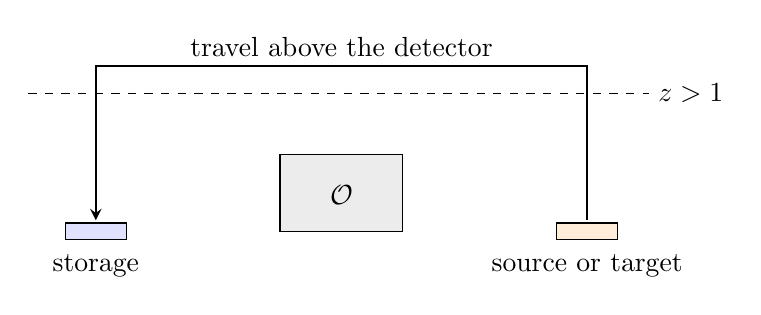
\begin{tikzpicture}[x=0.78cm,y=0.70cm,>=stealth]
 \draw[fill=gray!15] (4,0) rectangle (6,1.4);
 \node at (5,.65) {$\mathcal O$};
 \draw[fill=blue!12] (.5,-.15) rectangle (1.5,.15);
 \node[below] at (1,-.25) {storage};
 \draw[fill=orange!15] (8.5,-.15) rectangle (9.5,.15);
 \node[below] at (9,-.25) {source or target};
 \draw[->,thick] (9,.2)--(9,3)--(1,3)--(1,.2);
 \node[above] at (5,3) {travel above the detector};
 \draw[dashed] (-.1,2.5)--(10,2.5);
 \node[right] at (10,2.5) {$z>1$};
\end{tikzpicture}
\caption{Storage routing for a bounded detector, with the second
horizontal coordinate suppressed. All sources are evacuated before
any target is occupied. Scaling takes place at the storage positions;
horizontal travel takes place at height six. The drawing is schematic:
the storage and endpoint footprints are separated by the explicit
margins in Lemma~\ref{lem:sb-storage}.}
\label{fig:sb-storage}
\end{figure}

\subsection{Sheet and planar alternatives}
\label{subsec:sb-sheets}
When only a planar sheet carries the code, its vertical thickness can
be chosen after the horizontal motion. This allows a stronger path
statement: every horizontal coordinate of a tracked point can be made
a convex combination of its own endpoints. The widths in the two
horizontal directions need neither agree nor have equal products.  For source and target horizontal centers $a_i,b_i$ and half-widths $r_{ik}^0,r_{ik}^1$, interpolate the center and both half-widths by the same parameter $s$:
\[
 c_{i,\mathrm{hor}}=(1-s)a_i+sb_i,\qquad
 r_{ik}=(1-s)r_{ik}^0+sr_{ik}^1.
\]
Take starting height $z_0=1/4$ and private heights $z_i=1/2+i/(4(N+1))$.  Lift, interpolate, and lower on disjoint time stages.  A point of fixed fractional horizontal coordinates follows the convex combination of its own two endpoints.  The affine generator is
\[
 c_i'(t)+\operatorname{diag}\left(\frac{r'_{i1}}{r_{i1}},
 \frac{r'_{i2}}{r_{i2}},-\frac{r'_{i1}}{r_{i1}}-\frac{r'_{i2}}{r_{i2}}\right)(x-c_i(t)).
\]
This is exactly the reciprocal-normal-strain construction in Lemma~\ref{lem:sa-sheet-routing}, applied inside the open unit cube to the stated rectangles.  To verify its chart hypothesis for rectangles elsewhere than $[1/4,3/4]^2$, take one tenth of the minimum of $1$, the actual endpoint chart margins, the horizontal sup-norm gaps in the two endpoint families, and the private-height gaps.  The expanded plates then remain inside the cube and are separated by footprints during lift and lowering, and by height during interpolation.  The proof of that lemma consequently applies without a coordinate or viscosity normalization.

An invariant-plane realization solves a different problem. We first
allow the planar field to compress the rectangles to small squares,
route the squares through parking positions, and expand at the targets.
The lift will cancel its divergence in the normal direction.
For planar routing we use Lemma~\ref{lem:sa-planar-routing} with $D=(0,1)^2$ and the safe rectangle $G=(0,1/2)\times(0,1)$, or the right half of $D$ as specified below.  There are several explicit choices of the same finite path construction.  They preserve the full-rectangle affine maps but have their own smooth paths:
\begin{enumerate}
\item For the frontier sine plane, use initial contraction on $[0,1/4]$, $4N$ successive segment intervals on $[1/4,3/4]$, and expansion on $[3/4,1]$.  The contraction factors are $1-s+s\epsilon/r_{ik}$, and the expansion factors $1-s+sr'_{ik}/\epsilon$.  To avoid $l$ forbidden lines, select a vertex among $2l+3$ rational points $(a,1/4+a^2)$, $1/8<a<1/4$, also avoiding the two endpoints.  A line contains at most two such points.  Positive segment clearances give $\epsilon$ with moving and stationary squares separated by more than $10\epsilon$.
\item For the previous-tag plane, use $4N+2$ equal stages and logarithmic contraction and expansion.  Parking points have height half the minimum of all source and target center heights and abscissas $i/(2(N+1))$.  A two-segment vertex can be chosen below the finitely many forbidden rational lines: choose an abscissa below all positive vertical forbidden abscissas, then an ordinate below all positive intersections at that abscissa.  Include the line through the two endpoints among the exclusions.  With $\epsilon$ one hundredth of the minimum of $1$, side lengths, boundary margins, and squared line distances, $100\epsilon\le\min(1,d^2)\le d$.  A radial translation cutoff equal to one out to radius $2\epsilon$ and zero past $3\epsilon$ therefore misses every other tiny square of radius at most $\sqrt2\epsilon$.
\item For the shifted-start plane, choose all intermediate vertices in the right half.  A horizontal line below every endpoint and obstacle cannot coincide with any forbidden endpoint-obstacle line; avoiding their finitely many intersections gives a rational vertex.  Logarithmic contraction and expansion, with tiny half-side $\epsilon\le1/100$ and clearances greater than $10\epsilon$, keep a nonhalting point at first coordinate greater than $1/2-\epsilon>1/3$.
\item For the separator sine plane, use moving centers $c_i$ and half-size matrices $M_i$ throughout all stages, with linear interpolation during shrink and expansion.  Relative padded boxes $c_i+\lambda M_i[-1,1]^2$ are disjoint, and the field is
\[
 \sum_i\psi(M_i^{-1}(X-c_i))
     [c_i'+M_i'M_i^{-1}(X-c_i)].
\]
Here $\lambda=1+d_0/4$ with $d_0$ a positive endpoint margin/gap bound.  If $d_1$ bounds required boundary margins and $d_2\le1$ bounds the positive squared center separations along all planned segments, choose
$\epsilon=\tfrac12\min(m_0,d_1/\lambda,d_2/(4\lambda))$, with $m_0$ the minimum half-side.  Then padded tiny squares do not intersect, since their intersection would force center distance at most $2\sqrt2\lambda\epsilon<d_2$.  The path $c_i+M_i v$ is exact for every $v\in[-1,1]^2$.
\item For the two-cell-frontier plane, choose intermediate vertices on
$(1/8+r/8,1/8+r^2/8)$, $0<r<1$.  If there are $l$ forbidden lines, including the vertical lines through both endpoints, the $2l+1$ samples $r=j/(2l+2)$ include an admissible vertex.  A line intersects the parabola in at most two points.  Linear contraction and expansion and the one-hundredth clearance choice again prove full-rectangle transport and safe-region confinement.
\item For the zero-blank plane, choose a rational abscissa avoiding endpoint abscissas and vertical forbidden lines, then a rational ordinate avoiding the remaining line intersections.  Use fixed source/target cutoffs, linear contraction and expansion, and tiny half-side $\epsilon=d_*/10$, where $d_*$ is the minimum of $1$, half-sides, boundary margins and positive squared segment-to-obstacle distances.  Actual distances are at least $d_*$, while support and stationary-square radii sum to $3\sqrt2\epsilon<d_*$.  This includes boundary code points.
\end{enumerate}
In every case the first round moves all source centers to distinct parking positions before the second round occupies targets.  The cutoff equals one on a positive neighborhood of each tracked rectangle, or can be chosen with an arbitrarily smaller positive plateau collar without changing the field on that rectangle.  The exact formulas for the finite affine stages then apply on a positive initial neighborhood.  The stage fields vanish near stage endpoints, so they concatenate smoothly.  These verifications explain precisely why the planar-routing lemma applies to all the listed variants; no abstract extension of an unspecified code map is being assumed.

For the trigonometric variants put
\[
 U(X,z,t)=\left(\cos(2\pi z)b(X,t),
       -\frac{\sin(2\pi z)}{2\pi}\operatorname{div}_X b(X,t)\right).
\]
For the compact vertical variants use instead
\[
 U=(h'(z)b,-h(z)\operatorname{div}_X b),\qquad
 h(z)=(z-1/2)\chi(z),
\]
where $\chi=1$ on $[3/8,5/8]$ and is supported in $[1/4,3/4]$, periodically extended.  Lemma~\ref{lem:sa-invariant-lift} proves divergence cancellation, mean zero, and the exact planar motion on $z=0$ or $z=1/2$, respectively.  The same formula applies to a spatially constant planar loading field: its divergence is zero, and the horizontal mean vanishes after multiplication by $h'$.  Thus such loading does not need an unsupported compact planar chart assumption.

\section{Initialization and fixed observation regions}
\label{sec:sb-events}
A correct time-one instruction map does not yet prove a halting event.
We must locate the initial code, make the particle reach it from a fixed
label, and exclude the detector during every intermediate motion of a
nonhalting computation. We now prove
Theorem~\ref{thm:sb-realizations} by giving the actual placement and
checking the event for each of its rows.

\begin{proof}[Proof of Theorem~\ref{thm:sb-realizations}]
We specify the geometric data and check the all-time events in three groups.  Whenever one halting patch is specified, first merge the halting states as allowed above; this preserves the event, including initial halting.  The positive digit gaps remain valid at every closed rectangle edge.
In every case equation~\eqref{eq:sb-coded-map} makes the time-one map equal to the complete symbolic rule on its entire prefix rectangle.  For boxes and moving sheets, the stated affine formula holds on a three-dimensional neighborhood. For an invariant-plane construction, planar routing gives the formula on a planar neighborhood, and the lift reproduces that motion exactly on its invariant plane; no prescribed affine map off that plane is inferred.  Smooth flat collars allow the chosen pulse to be repeated every unit interval while preserving $U(0)=0$.

\emph{Euclidean full boxes.}
For left-word boxes use Lemma~\ref{lem:sb-postlog} with initial stacks $\#^\infty,w\square^\infty$, the odd-digit base $2m+2$, and state offsets $o_s$ given by distinct positive multiples of $3$ for nonhalting labels and distinct negative multiples for halting main labels.  The spatial code is $(o_s+c(L),c(R),0)$.  Use the relative-padding private-height construction following Lemma~\ref{lem:sb-boxes}, and load the rational initial code from the origin by a localized straight translation during $[0,1]$.  A cutoff with a unit-box plateau and a larger compact support suffices.  At a halt the first coordinate is at most $-2$.  On every nonhalting instruction both endpoint centers have first coordinate at least $3$, while the first half-width is at most $1/2$ throughout the period.  The entire path is therefore positive in that coordinate.  A nonhalting loading segment is nonnegative.  This proves the first row.

For right-word boxes use Lemma~\ref{lem:sb-rightword}, even digits in base $2m$ with blank digit zero, offsets $-2j$ for the $j$th halting state and $2j$ for the $j$th other state, both numbered from $1$.  The initial code is $(o_{q_0},b(w\square\#),0)$.  The full-box data have unit source half-height and reciprocal target half-height, and use exactly the additive-gap construction of Lemma~\ref{lem:sb-boxes}.  Initialize by the same lemma for one translated unit cube with all scales equal to one.  Its initial and final centers have height zero, although the loading path rises and descends; its first coordinate still interpolates from zero to the initial code.  Halting gives first coordinate at most $-1$.  Nonhalting rule centers are at least $2$ and half-widths at most $1/2$, excluding $x_1<-1/2$ at all times.

For tagged storage use Lemma~\ref{lem:sb-tagged}, digits $1,4,\ldots,3m-2$ in base $3m$, and offsets $o_s=3\operatorname{index}(s)$ with the halting main state indexed zero.  Use the thin boxes and $7N$-slot storage pulse of Lemma~\ref{lem:sb-storage}.  Load from $(-4,0,0)$ by three localized translations through
\[
 (-4,0,0),\quad(-4,0,6),\quad a_{\rm in}+(0,0,6),\quad a_{\rm in}.
\]
Take unit-box plateaus and margin $1/4$ for these loading pulses.  A nonhalting initial code has first coordinate at least $3$, so the vertical loading legs are outside the observation box and the horizontal leg is at height $6$.  The storage lemma excludes it on every later nonhalting period.  At a halting code both horizontal coordinates belong to $(0,1)$ and the height is zero, so the code lies strictly inside the observation box.

For boot-window prisms use Lemma~\ref{lem:sb-window}, base $2m+2$ with even digits and $d(E)=0$, offset $2$ for the halting main state, and distinct negative offsets $-3k$ for all others, with boot offset $-3$.  The initial code is exactly $(-3,0,0)$.  Include the boot rule in the full-box pulse, using the private heights $4(R+1)i$ and padding specified above.  Thus there is no loading interval outside the period.  Halting codes have first coordinate in $[2,3]$.  Every nonhalting endpoint footprint lies at first coordinate at most $-2$; the center interpolation and half-width bound keep the whole moving box strictly negative.  This proves the four Euclidean rows, including the initial-halt cases at time $1$ after loading or boot.

For tagged storage, uniqueness also holds under the pointwise comparison bounds
\[
 u,\partial_tu,\nabla u,\nabla^2u,p,\nabla p
       =O((1+|x|)^{-2})
\]
uniformly on every finite time interval, with pressure decaying at infinity.  Smoothness and these bounds imply the Sobolev and time-continuity requirements of Section~\ref{sec:model} by dominated convergence; $\partial_tu\in C_tL^2$ gives $C_t^1L^2$.  Hence the stated uniqueness includes this entire comparison class.  For the other Euclidean rows, a pressure representative in $C_tH^1$, modulo spatial constants when applicable, is the normalization specified in the theorem.  The constructed compactly supported velocity and zero pressure satisfy all these conventions.

\emph{Reserved-loader sheets.}
Both sheet rows use the post-update processor of Lemma~\ref{lem:sb-postlog}, with an additional history symbol $h_*$ unused in any ordinary rule.  For the left reserved sheets, place the halting interval at $[5/32,7/32]$ and enumerate the $J$ other states by $j=0,\ldots,J-1$ with intervals
\[
 [1/2+(3j+1)/(12J),\ 1/2+(3j+2)/(12J)].
\]
Use second interval $[1/4,3/4]$ and height $1/4$.  The input target is the code in $U_{q_0}$ of
$\#h_*\#^\infty,\diamond w\square^\infty$.
It lies in the interior of the unused image cylinder with prefixes $(\#h_*,\diamond)$.  Indeed the incoming $U_{q_0}$ images have left prefix $c\in A$ or $\#h_i$, never $\#h_*$.  A rational square centered at this target, with half-side half its minimum coordinate distance to the four cylinder edges, is therefore disjoint from every ordinary target.  Add a source square centered at $(1/2,1/2)$ with half-side half the minimum of $1/4$ and its positive distances in the first coordinate to the state intervals.  This source is disjoint from every ordinary source.  The positive affine source-to-target map supplies a loader in the same repeated pulse.

For the right reserved sheets, use the same table with history tail $h_*\square^\infty$, halting interval $[13/16,7/8]$, second interval $[1/4,1/2]$, and height $1/4$.  If $S$ is the number of other labels, put $\delta=1/(8(S+1))$ and give label $l=1,\ldots,S$ the first interval
\[
 [1/8+2(l-1)\delta,\ 1/8+(2l-1)\delta].
\]
These lie strictly below $3/8$.  The loader source is the square at $(1/2,1/8)$ with half-side $1/32$.  Its target is the code of $(U_{q_0},\#h_*\square^\infty,\diamond w\square^\infty)$, surrounded by the same half-minimum-margin square inside its reserved cylinder.  The same prefix argument proves separate disjointness of both enlarged instruction families.

Apply the moving-sheet construction to each placement.  The reciprocal normal strain is trace-free, all supports lie in the unit cube, and each horizontal coordinate of a tracked sheet point is a convex combination of its own endpoints.  At integer time $1$ the fixed particle is at its reserved $U$-code, and at time $2$ the ordinary marker-removal instruction gives the initial main configuration.  A machine halting initially is therefore detected at $2$.  Otherwise the main times satisfy
$t_0=2$, $t_{j+1}=t_j+2|L_{j+1}|+3$.
For the left placement, loading and all nonhalting endpoints lie at first coordinate at least $1/2$, and subsequent state intervals are in $(1/2,3/4)$.  For the right placement the loading point has coordinate $1/2$ and all nonhalting state intervals are below $3/8$.  Convex interpolation excludes the corresponding observation arcs throughout every period.  Halting state intervals are strictly inside the displayed arcs.  Periodicity starts at zero because the same loader is present in every pulse, with no image collision.

\emph{Invariant-plane realizations.}
For the frontier sine plane use Lemma~\ref{lem:sb-frontier}, its two-stack conversion, and odd digits in base $2m+1$.  With $P$ the auxiliary label set, put $s=1/(8|P|)$ and choose an index $i(p)\in\{0,\ldots,|P|-1\}$ for each label.  Use state squares with lower-left corners
\[
 o_p=(1/8+2s i(p),1/2)\quad(p\ne B_H),\qquad
 o_{B_H}=(3/4,1/2),
\]
and side $s$.  Nonhalting squares lie in $0<x_1<3/8$; the halt square lies in $[3/4,7/8]$.  Use the first planar routing choice above and the sine lift.  Load the rational initial code from $(1/2,1/4)$ along its straight segment, using a translated square cutoff with plateau half-side $1/32$ and support half-side $1/16$.  Both endpoints have chart margins at least $1/8$.  Nonhalting loading has first coordinate at most $1/2$, and every later nonhalting rectangle path remains in the left half.  Thus the event is exact.  The main checkpoint times are
\[
 t_0=1,\qquad t_{n+1}=t_n+2(2+n-h_{n+1})+4.
\]

For the previous-tag plane use Lemma~\ref{lem:sb-prelog} and odd digits in base $2m+1$.  Let $r=c(\square^\infty)$ and place the input rectangle at
\[
 [1/8-r/16,1/8-r/16+1/16]\times
 [1/4-r/8,1/4-r/8+1/8].
\]
Thus the two blank stacks have code exactly $(1/8,1/4)$.  Halting $B$-labels have disjoint first intervals inside $(2/3,5/6)$; all other noninput labels have them inside $(1/4,1/2)$, with common second interval $[1/4,1/2]$.  To place $n$ labels in $(a,b)$, take interval $[a+(2j-1)d,a+2jd]$, $j=1,\ldots,n$, $d=(b-a)/(2n+1)$.  Use the logarithmic planar shrink and expansion of the second routing choice and the sine lift.  The loader is already a disjoint prefix rule, so period one begins at zero.  The first main time is $t_0=1$, and the next is $t_{j+1}=t_j+2|L_j|+4$.  Every rule whose source and target are both nonhalting, including the loader when its target is nonhalting, has both rectangles in the left half and stays there throughout its pulse.  Halting main rectangles lie inside the observation arc.

For the shifted-start plane, prepend a fresh nonhalting state $q_s$ which writes back the scanned symbol and stays while entering the original initial state.  Apply Lemma~\ref{lem:sb-frontier} to this enlarged table.  This fresh state is different from the halt state even if the original machine halts initially.  Compute the rational initial normalized stack coordinates $(\xi_0,\eta_0)$, using blank combined-symbol tails and a history frontier at $2$.  If $L$ is the number of auxiliary labels, set $\ell=1/(16(L+1))$.  Put the halt square at lower-left corner $(1/8,1/2)$, the fresh-start square at
\[
 (3/4,3/4)-\ell(\xi_0,\eta_0),
\]
and the other squares at $(1/2+(2k+1)\ell,1/2)$, $k=0,\ldots,L-3$, all of side $\ell$.  These are disjoint; the initial code is exactly $(3/4,3/4)$, independently of the input.  The ordinary nonhalting squares lie in $1/2<x_1<5/8$, the start square near $(3/4,3/4)$, and the halt square lies inside $0<x_1<1/3$.  Use the third routing choice, with the right half as the safe region and tiny half-side at most $1/100$, then the compact vertical lift about $z=1/2$.  Nonhalting paths have first coordinate greater than $1/3$ throughout.  The repeated field starts at zero and is periodic from zero, with no separate loader.  The extra initial machine transition is simulated in finitely many periods, so initial halting of the given machine is still detected.

For the separator sine plane use Lemma~\ref{lem:sb-postlog} with initial stacks $\#\square^\infty,w\square^\infty$.  The nonhalting state rectangles, indexed $j=1,\ldots,n$, are
\[
 [(3j-2)/(6n),(3j-1)/(6n)]\times[1/4,3/4],
\]
and the halting rectangle is $[2/3,5/6]\times[1/4,3/4]$.  Use odd digits in base $2m+1$, the moving-center/moving-cutoff fourth routing choice, and the sine lift.  A spatially constant planar pulse takes $(1/4,1/2)$ along the straight segment to the rational initial code during $[0,1]$.  Both endpoints lie in the left half when the initial state is nonhalting, so this loading is safe.  Thereafter nonhalting rectangles and their paths remain in the left half; a halt code enters $(1/2,1)$.  The main times are $1+\sum_{j=1}^k(2|L_j|+3)$.

For the two-cell-frontier plane use Lemma~\ref{lem:sb-neighbor}, odd digits in base $2m+2$, and its complete three-cell branch list.  If $N$ is the number of nonterminal auxiliary labels, set $\ell=1/(16(N+1))$, put their square origins at $(1/4+2i\ell,1/4)$, $i=0,\ldots,N-1$, and the terminal origin at $(3/4,1/4)$, all with side $\ell$.  All source squares belong to nonterminal labels and lie in the left half; the halt square lies strictly in the observation arc.  Apply the rational-parabola fifth routing choice and the sine lift.  A compact planar loading pulse takes $(1/8,1/8)$ to the initial code along its segment, with plateau half-side $1/64$ and support half-side $1/32$.  The chart margins make this legal, including when initially halted.  Nonhalting loading and all nonhalting branches remain in the left half.  The main checkpoint recurrence is
$t_0=1$, $t_{n+1}=t_n+2(2+n-h_{n+1})+2$.

Finally, for the zero-blank plane use Lemma~\ref{lem:sb-postlog}, initial stacks $\#\square^\infty,w\square^\infty$, and even digits in base $2m+1$ with blank digit zero.  The $N$ nonhalting state squares have centers $(j/(2(N+1)),1/2)$, $j=1,\ldots,N$, and half-side $1/(8(N+1))$.  The halting square has center $(13/16,1/2)$ and half-side $1/32$.  Apply the fixed-cutoff sixth planar routing choice, then the compact vertical lift about $z=1/2$.  The initial normalized code is rational even when on a prefix boundary.  A spatially constant planar translation loads it from $(1/4,1/2)$; that segment stays in the left half in a nonhalting run.  All subsequent nonhalting paths stay there as well, while the halt square lies strictly inside $(3/4,7/8)$.  The checkpoint count is again $2|L_j|+3$ per transition after loading.

For all rows, induction on individual instruction periods now gives the exact encoded auxiliary configuration at each integer boundary through the first halt, or indefinitely in a nonhalting run.  The processor lemmas group those samples into the stated machine checkpoints, each after a finite positive number of instructions.  In an infinite run the times tend to infinity, so the all-time exclusions just proved cover every time.  After reaching a halted code no further symbolic rule is needed; the smooth fluid motion continues globally.  The state rectangles and separated digit intervals recover every finite prefix of both words, hence the represented configurations and their recorded head displacements.

All geometry and initial codes are obtained by finite symbol manipulation and rational arithmetic.  Smooth switches, logarithms of positive rational scales, finite differentiations, and bounded-index periodization give effective mixed-derivative evaluation as in Section~\ref{sec:model}.  At no point does constructing or evaluating the force require knowing the successive rules selected by the marked point.  The finite pulse acts on every branch domain during every period.  The residual realization lemma proves the claimed Navier--Stokes solution and comparison uniqueness.  Compact support or spatial periodicity and the repeated finite pulse give uniform derivative and energy bounds.

For the solenoidal alternative in the separator sine-plane row, apply Proposition~\ref{prop:projection-l2} to its mean-zero residual force.  If $\Delta r=\operatorname{div}f$ and $\int r=0$, replace $f$ by $f-\nabla r$ and the pressure by $-r$.  In Fourier coordinates,
\[
 r_k(t)=-\frac{\widehat{\operatorname{div}f}(t,k)}{4\pi^2|k|^2},\qquad k\ne0,
 \qquad r_0=0.
\]
Integration by parts gives arbitrarily high inverse-power coefficient bounds for every requested time derivative.  The shell $\|k\|_\infty=l$ contains $24l^2+2$ modes, so sufficiently many spatial derivatives provide effective summable tails for every derivative of $r$.  The projection preserves period one after loading, mean zero, and bounded derivatives, and leaves the velocity and its event unchanged.
\end{proof}

\subsection{Logarithmic clocks for the compact box constructions}
\label{subsec:sb-clock}
The periodic forces above and the following decaying forces are separate choices.  A reparametrization changes speed, while preserving every point of the material trajectory.

\begin{proposition}[Logarithmic alternatives]\label{prop:sb-log}
For each of the left-word-box, right-word-box, and tagged-storage constructions, retain its fixed initial label and observation set.  There is also an effective smooth force of fixed compact spatial support in
$L^2([0,\infty)\times\mathbb R^3)$ with exactly the same halting event and zero initial velocity.  It and all its derivatives are bounded.  The velocity's spatial derivatives are $O((1+t)^{-1})$, and their first time derivatives are $O((1+t)^{-2})$, uniformly in space.  The force itself is $O((1+t)^{-1})$ uniformly in space. The viscosity
in this statement is the same fixed physical $\nu$ as before the time
change.
\end{proposition}
\begin{proof}
Write $U(s,x)$ for the chosen construction, including its loading
interval. It is periodic only after that interval, but all its derivatives
are uniformly bounded on the whole half-line. Put
\[
 s(t)=\log(1+t),\quad a(t)=(1+t)^{-1},\quad
 \widehat U(t,x)=a(t)U(s(t),x).
\]
It is smooth and effective and has the same spatial support.  Since $U(0)=0$, its initial velocity is zero.  For every spatial multi-index $\alpha$,
\[
 \partial_x^\alpha\widehat U=a(\partial_x^\alpha U)\circ s,
 \qquad
 \partial_t\partial_x^\alpha\widehat U
   =a'(\partial_x^\alpha U)\circ s
       +a^2(\partial_s\partial_x^\alpha U)\circ s.
\]
The uniform derivative bounds for the original finite pulse give the stated spatial and first-time estimates.  Repeated chain and product rules express every higher mixed derivative as a finite sum of bounded derivatives of $U$ multiplied by derivatives of $a$ and $s$, so all are bounded as well.  The new residual force is exactly
\[
 \mathcal F_\nu[\widehat U]
  =a'U\circ s+a^2\big(\partial_sU+(U\cdot\nabla)U\big)\circ s
                -\nu a(\Delta U)\circ s.
\]
Its pointwise magnitude is at most $C(1+t)^{-1}$.  Fixed compact support gives a finite space-time square integral, since $\int_0^\infty(1+t)^{-2}\,dt<\infty$.  The same realization and uniqueness argument applies.  If $X(s)$ was the original material path, then $X(s(t))$ solves the new particle ODE by the chain rule.  The clock is increasing and maps $[0,\infty)$ onto itself, so the two paths have identical images and exactly the same observation event.  A checkpoint at original time $s_j$ is reached at the finite new time $e^{s_j}-1$; no finite upper bound on the halting time is required to prescribe this clock.
\end{proof}

\section{Two compact realizations of the reciprocal recorder}
\label{subsec:p2:rapid-periodic}
The preceding area-changing constructions use the third coordinate to
compensate a planar determinant. For the ordinary one-head recorder,
the planar maps already have determinant one. The third coordinate can
then serve only to separate instructions during transport. We give two
compact Euclidean realizations: one uses four stationary fields in
succession, and the other follows entire moving boxes in three phases.
Their observer estimates will follow directly from the horizontal
motion, without a vertical restriction on the detector.

Use the frontier recorder of Lemma~\ref{lem:sb-frontier} throughout this
section. Its frontier starts at absolute cell two; every other history
cell is blank and every return mark is zero. Its fixed incoming moves
and distinguishing written symbols will separate the target rectangles.
At checkpoint $k$ the records occupy $2,\ldots,k+1$, the frontier is at
$k+2$, and transition $k+1$ takes $2(k+2-h_{k+1})+4$ instructions.
These properties hold for the same entire partial table as in that lemma.

Choose the combined alphabet $\mathcal A$ of the recorder, of size $m$.
Give its letters the even digits $g_a=0,2,\ldots,2m-2$, with the fully
blank combined letter first. We will use either $B=2m$ or $B=2m+1$.
For a tape $v$ whose head is at its relative index zero, set
\[
 x=\sum_{j\ge1}g_{v_{-j}}B^{-j},\qquad
 y=\sum_{j\ge0}g_{v_j}B^{-j-1},\qquad
 I_a=[g_a/B,(g_a+1)/B].
\]
These are the gapped codes of Section~\ref{subsec:sb-codes}.
A state $s$ is placed at $(o_s+x,y,0)$ for a specified offset $o_s$.
If a rule reads $a$, writes $b$, moves by $d$, and enters $s'$, its
coordinate map relative to the source and target offsets is
\begin{equation}\label{eq:p2:rapid-rectangle-rules}
\begin{array}{c|c|c}
 d&\text{source rectangle}&(x',y')\\\hline
 1 &[0,1]\times I_a&((g_b+x)/B,\ By-g_a)\\
 0 &[0,1]\times I_a&(x,\ y+(g_b-g_a)/B)\\
 -1&I_\ell\times I_a&
 (Bx-g_\ell,\ (g_\ell+(g_b+By-g_a)/B)/B).
\end{array}
\end{equation}
For the last row there is one branch for each $\ell\in\mathcal A$.
The target rectangles are respectively $I_b\times[0,1]$,
$[0,1]\times I_b$, and $[0,1]\times(g_\ell/B+I_b/B)$.
These formulas follow by removing the scanned digit and pushing the
written digit. They apply to every point of the displayed closed
rectangles. Determinism separates the sources; the fixed incoming
displacement and distinguishing written symbol separate the targets.
For a left move the target pair $(\ell,b)$ supplies that distinction.
Every linear part is $\operatorname{diag}(\lambda,\lambda^{-1})$.

The code also retains absolute, rather than only head-relative,
configuration information at the machine checkpoints. Count the records
immediately to the left of the frontier to recover $k$. The frontier
has absolute position $k+2$; its location in the decoded tape therefore
recovers the absolute head position. The work track then recovers the
original tape. This use of history records is the retained-history
version of the reversible-computation idea of Bennett~\cite{Bennett1973};
the positional affine representation follows the generalized-shift
viewpoint of Moore~\cite{Moore1990,Moore1991}.

\begin{proposition}[Two compact periodic processors]
\label{prop:p2:rapid-periodic}
For every deterministic machine and finite input, and every fixed
computable viscosity $\nu>0$, there are effective smooth velocities
$U$ and forces $f$ on $\mathbb R^3$ with the following properties.
Both have all mixed derivatives bounded, support in a compact spatial
set independent of time, and period one for $t\ge1$; $U(0)=0$.
The solution with pressure zero is unique in the class
\[
 u\in C([0,T];H^2)\cap C^1([0,T];L^2),\qquad
 p\in C([0,T];H^1),\qquad
 \sup_{[0,T]\times\mathbb R^3}(|u|+|\nabla u|)<\infty
\]
for every finite $T$, and its kinetic energy is uniformly bounded.
The following are two separate constructions with their stated fixed
particle events:
\begin{enumerate}
\item Four successive stationary localized fields, with initial label
$(-1,0,0)$ and detector $\{x_1>0\}$.
\item Three successive phases of moving full-box fields, with initial
label $(0,0,0)$ and detector \mbox{$\{x_1<-1\}$}.
\end{enumerate}
In each case the particle enters the detector at some real time if and
only if the machine halts. The repeated part of the prescription depends
only on the machine; the input appears only in a one-time loading pulse.
\end{proposition}
\begin{proof}
Let $R_i,R_i'$ be the planar source and target rectangles in
\eqref{eq:p2:rapid-rectangle-rules}, with centers $c_i,c_i'$ and first
scale $\lambda_i$. All their side lengths are at most one. If there are
no instructions, use the zero repeated field and the same loader described
below. Empty pairwise margin tests are omitted for a singleton family.

For the first realization choose $B=2m$. Put terminal offsets at
$4,7,10,\ldots$ and all other offsets at $-4,-7,-10,\ldots$.
Choose private heights $h_i=4i$. On four successive quarters of a unit
period, perform the following autonomous motions, each with flat progress
from zero to one:
\begin{enumerate}
\item Translate upward by $h_i e_3$, with a cutoff equal to one near
$R_i\times[0,h_i]$.
\item At height $h_i$, use the Hamiltonian vector potential
\[
 (0,0,\chi_i\log(\lambda_i)
                (X_1-c_{i1})(X_2-c_{i2})).
\]
Its curl on the plateau is
$\log(\lambda_i)(X_1-c_{i1},-(X_2-c_{i2}),0)$.
\item Translate horizontally by $c_i'-c_i$ at height $h_i$.
\item Translate downward by $h_i e_3$ near $R_i'\times[0,h_i]$.
\end{enumerate}
A translation by $w$ is localized by
$\operatorname{curl}(\chi(w\times X)/2)$.
In the first and last quarters, choose cutoff collars below one third
of the smallest positive horizontal separation in the source and target
families, respectively. In the middle quarters, collars of thickness
one in height do not meet because the heights differ by four. For the
stretch, choose the horizontal plateau to include
$c_i+[-1,1]^2$. For translation, include the bounding rectangle of
$[c_i,c_i']$ enlarged by one in each horizontal direction.

More explicitly, with $\vartheta(s)=\sigma(2s-1/2)$ and
$\vartheta_j(s)=\vartheta(4s-j+1)$, multiply the sum of the stationary
fields for quarter $j$ by $\vartheta_j'(s)$. The tracked rectangle rises,
scales by $(\lambda_i^{\vartheta_2},\lambda_i^{-\vartheta_2})$,
translates its center along $[c_i,c_i']$, and descends. Each intermediate
half-width is at most $1/2$, so the entire rectangle remains on the
specified plateaus. The positive collars and finite affine norms also
give exactness on a positive initial neighborhood. If both endpoint
states are nonterminal, both first center coordinates are at most
$-3$, and the whole tracked path has negative first coordinate.

For the second realization choose $B=2m+1$, nonterminal offsets
$3,6,9,\ldots$, and terminal offsets $-3,-6,-9,\ldots$.
Thicken each rectangle by $[-1,1]$ in height, and write $c_i^0,c_i^1$
for the three-dimensional endpoint centers. Each pair within the
source family, and within the target family, has a horizontal coordinate
gap at least $B^{-2}$. Use height $6i$ and collar
$\epsilon=1/(4B^2)$. In three successive phases the prescribed affine
paths have center and linear part
\[
\begin{array}{c|c|c}
 &c_i(s)&L_i(s)\\\hline
 \text{lift}&c_i^0+6i\Theta e_3&I\\
 \text{transfer}&(1-\Theta)c_i^0+\Theta c_i^1+6i e_3&
     \operatorname{diag}(\lambda_i^\Theta,\lambda_i^{-\Theta},1)\\
 \text{lower}&c_i^1+6i(1-\Theta)e_3&
     \operatorname{diag}(\lambda_i,\lambda_i^{-1},1),
\end{array}
\]
where $\Theta$ is $\vartheta$ rescaled to the active third.
The proof of Lemma~\ref{lem:sb-boxes} applies to these exact data:
horizontal gaps separate the collars during lift and lowering, while
height gaps six separate vertical half-widths $1+\epsilon$ during
transfer. The localized field is explicitly
\begin{equation}\label{eq:p2:rapid-moving-box}
 \sum_i\operatorname{curl}_X\left[
 \chi_i\left\{\frac{\dot c_i\times(X-c_i)}2+
       \frac{(\dot L_iL_i^{-1}(X-c_i))\times(X-c_i)}3\right\}\right].
\end{equation}
The trace of $\dot L_iL_i^{-1}$ is zero. The curl identity in
Lemma~\ref{lem:sa-curl-motion} therefore gives the prescribed affine
velocity near each moving box, and ODE uniqueness gives its exact
full-box motion. A branch with two nonterminal endpoint states has
first center coordinate at least three and half-width at most $1/2$;
hence its entire path has first coordinate at least $5/2$.

It remains to initialize and to pass from the finite maps to the fluid
event. The initial combined tape is blank except at finitely many cells,
so its initial code $Z_0$ is rational. During $[0,1]$, a localized curl
translation with flat progress carries the fixed label to $Z_0$ along
the straight segment. A compact cutoff contains the whole segment with
a positive collar. Repeat the chosen instruction pulse on every later
unit interval. The time collars make all joins smooth, and only
finitely many spatial supports occur. Thus $U$ has the support and
derivative bounds in the statement. Set
\[
 f=\partial_tU+(U\cdot\nabla)U-\nu\Delta U.
\]
The residual realization and comparison argument of
Section~\ref{sec:model} gives the asserted solution and uniqueness;
fixed support and bounded $U$ give bounded kinetic energy. The formula
can also be returned as $f=f^{(0)}+\nu f^{(1)}$, with
$f^{(0)}=U_t+(U\cdot\nabla)U$ and $f^{(1)}=-\Delta U$ effective
independently of $\nu$. Evaluation for an arbitrary fixed real viscosity
is relative to that parameter.

At each integer $1+j$ through a halt, or at every such integer in a
nonhalting run, the particle is the exact code after $j$ auxiliary
instructions. Lemma~\ref{lem:sb-frontier} supplies finite positive
instruction counts between the original machine checkpoints. In the
first realization, a nonhalting loading segment has negative first
coordinate, and all subsequent nonterminal branches stay negative;
a terminal code has positive first coordinate. In the second,
nonhalting loading has nonnegative first coordinate and later
nonterminal paths stay above $5/2$ in that coordinate, while a terminal
code has first coordinate at most $-2$. An initially halted machine is
detected at the end of loading. Thus the exclusions apply at every real
time, and a halting run enters the detector no later than its terminal
checkpoint. No exclusion is needed during a final transition into a
terminal state.

All rectangles, cutoffs, scales and finite branch fields are computed
from the finite table. Positive rational scales have effective logarithms
and exponentials. Smooth switching and derivative bounds permit
evaluation at time joins without equality tests. The finite repeated
field acts on all branch domains at every period; neither its definition
nor its evaluation uses a predicted sequence of machine configurations.
\end{proof}

\section{An autonomous processor with a spatial clock}
\label{sec:sa-autonomous}
The preceding constructions repeat a time-dependent pulse.  We now make
that repetition part of an autonomous divergence-free field: a third
coordinate runs through the phases of a planar Hamiltonian motion.
The observer is restricted to a quiet clock window, so transient transport
paths cannot give false detections.  An onto scalar time change then starts
the fluid from rest and makes its force decay.

\begin{theorem}\label{thm:sa-autonomous}
At fixed positive computable viscosity, a deterministic one-tape machine
and finite input effectively determine a smooth mean-zero general force
on the unit torus such that, for every $k\ge0$ and spatial multi-index
$\beta$,
\begin{equation}\label{eq:sa-autonomous-force-class}
 \|\partial_t^k\partial_x^\beta f(t)\|_\infty
       \le C_{k,\beta}(1+t)^{-1}.
\end{equation}
Its zero-data Navier--Stokes solution is globally smooth and unique in
the classical periodic comparison class, with uniformly bounded kinetic
energy and mean-zero pressure.  For the fixed label and open set
\begin{equation}\label{eq:sa-autonomous-event}
 y_*=(1/2,1/2,1/4),\qquad
 \mathcal O=\{(x_1,x_2,z):1/2<x_1<1,\ 0<z<1/8\},
\end{equation}
its material trajectory enters $\mathcal O$ exactly when the machine
halts.  Samples encode the full machine computation through the first
halt, or indefinitely if there is none.  The prescription uses only the
finite table and input; arbitrary fixed real positive viscosity is allowed
as a relative coefficient.
\end{theorem}

\subsection{A recorder with identifiable incoming instructions}
\label{subsec:sa-autonomous-processor}
Normalize to one halt state $q_f$ and a total nonhalt table.  Add a fresh
initial state $q_I$ whose instructions preserve the symbol, stay put,
and enter the old initial state.  No rule enters $q_I$.  This guarantees
a positive number of steps before any halt and ensures that the initial
control is never visited again.  Let $Q$ and $A$ be the normalized
state set and work alphabet.
Apply the frontier recorder of Lemma~\ref{lem:sb-frontier} to this
normalized ordinary machine, using exactly its notation:
\[
 \mathcal R=(Q\setminus\{q_f\})\times A,\qquad
 \Sigma=A\times\{\mathtt e,\mathtt F,\lambda_r:r\in\mathcal R\}
                  \times\{0,1\}.
\]
The main controls are $B_q$; the other controls are $A_r,R_r,N_q,L_q$.
At a main checkpoint the work track represents the ordinary tape, all
return marks vanish, and a rightward frontier follows the finite history
block. One ordinary step writes and moves the work head, marks its new
position, records the instruction at the frontier, advances that frontier,
and returns to the marked position. Lemma~\ref{lem:sb-frontier} proves
this cycle and its full-domain inverse with every nonfrontier guard.
In particular each target control has a fixed incoming displacement and
the written whole symbol determines its incoming instruction. These are
the precise hypotheses used for the reciprocal rectangles below.

Initialize at $B_{q_I}$, head zero, with the input work tape, all marks
zero, history frontier $\mathtt F$ at cell two and $\mathtt e$ elsewhere.
At the $n$th ordinary checkpoint, after primitive count $m_n$, the work
configuration is the normalized machine's $n$th configuration, records
occupy cells $2,\ldots,n+1$, and the frontier is at $n+2$.
If $h_{n+1}$ is the new work-head position, the same lemma gives
\begin{equation}\label{eq:sa-autonomous-count}
       m_{n+1}-m_n=2(n+2-h_{n+1})+4.
\end{equation}
Thus each ordinary step takes finitely many positive primitive steps.
The fresh state $q_I$ occurs only at the initial ordinary checkpoint,
and at least one ordinary step precedes any halt. In a nonhalting run
no positive primitive sample has main control $B_{q_f}$ or $B_{q_I}$.

\subsection{Reciprocal rectangle maps}
\label{subsec:sa-autonomous-rectangles}
Use odd digits and base $K=2|\Sigma|+1$ in Lemma~\ref{lem:sa-radix}.
For a tape relative to its head let
$x=E(\sigma_{-1}\sigma_{-2}\cdots)$ and
$y=E(\sigma_0\sigma_1\cdots)$, and encode by $o_r+(x,y)$.
The two internal initial coordinates $x_{\rm in},y_{\rm in}$ are
rational.  Choose
\begin{equation}\label{eq:sa-autonomous-offsets}
 o_{B_{q_I}}=(-x_{\rm in},-y_{\rm in}),\qquad
 o_{B_{q_f}}=(2,0),\qquad o_r=(-3j,0)\quad(j=1,2,\ldots)
\end{equation}
for the remaining controls.  The initial code is zero, and the closed
state squares $o_r+[0,1]^2$ are disjoint.

For an instruction $(r,\eta)\mapsto(r',\beta,d)$ write
$h_\sigma(v)=(d(\sigma)+v)/K$.  The normalized branches are
\begin{equation}\label{eq:sa-autonomous-branches}
\begin{array}{ll}
 d=0:&(x,h_\eta(v))\mapsto(x,h_\beta(v)),\\
 d=1:&(x,h_\eta(v))\mapsto(h_\beta(x),v),\\
 d=-1:&(h_\gamma(w),h_\eta(v))\mapsto
          (w,h_\gamma(h_\beta(v))),\quad\gamma\in\Sigma.
\end{array}
\end{equation}
All free variables range independently over $[0,1]$.
These are exactly the head-relative list operations.  Sources are
separated by control, read symbol, and the extra left symbol for a left
move.  For a common target control the incoming move is fixed and distinct
rules have distinct written symbols.  Those symbols separate the right
first digit for a stay, the left first digit for a right move, and the
right pair $(\gamma,\beta)$ for a left move.  Thus targets are separately
separated as well.  The linear parts are $I$, $\diag(1/K,K)$, and
$\diag(K,1/K)$, respectively.  Unlike general prefix maps, all preserve
planar area.  This leaves the third coordinate available for a clock.

\subsection{A Hamiltonian extension without planar contraction}
\label{subsec:sa-autonomous-extension}
The area-preserving requirement rules out the simultaneous contraction
used in Lemma~\ref{lem:sa-planar-routing}.  Instead we separate the
rectangle centers, carry the unchanged rectangles to distant parking
positions, and deform them there with reciprocal scales.

\begin{lemma}\label{lem:sa-autonomous-extension}
Let $U_i,\widehat U_i$, $1\le i\le J$, $J\ge1$, be two separately
disjoint families of nondegenerate rational closed rectangles in
$\mathbb R^2$.  For each pair prescribe
\[
 X\mapsto\widehat c_i+
       \diag(\lambda_i,\lambda_i^{-1})(X-c_i),\qquad\lambda_i>0
\]
with rational $\lambda_i$ and the respective centers, and require the
compatibility condition
\[
 \widehat U_i=\widehat c_i+
       \diag(\lambda_i,\lambda_i^{-1})(U_i-c_i).
\]
There is an effective smooth compactly supported planar Hamiltonian
field $V(\xi,X)$, with time support in $(1/4,3/4)$, whose unit-time
map has this formula on each $U_i$ and a positive neighborhood.
The construction gives a rational bound on its spatial support and all
controlled rectangle paths.
\end{lemma}
\begin{proof}
Choose a positive rational margin $\epsilon$ at most one quarter of a
positive coordinate-separating gap for each pair in each family; for
empty pair lists take $\epsilon=1$.  The enlarged families stay disjoint.
Choose rational $D_0$ larger than $\epsilon$ plus every source or target
half-side.  Take an integer $G\ge1$ so that within each family the
scaled centers $Gc_i$ and $G\widehat c_i$ are more than $10D_0$ apart
in the sup norm.  Choose parking centers $e_i$ more than $10D_0$ apart
from one another and from all these scaled centers.  A sufficiently
distant row with spacing $20D_0$ does this effectively.

Use affine paths
\begin{equation}\label{eq:sa-autonomous-moving-box}
 X\mapsto C_i(\xi)+\diag(a_i(\xi),a_i(\xi)^{-1})(X-c_i).
\end{equation}
First translate centers simultaneously $c_i\to Gc_i$, keeping shapes
fixed; any coordinate separation can only increase.  Next move one
rectangle at a time to $e_i$.  At those parking centers change $a_i$
from $1$ to $\lambda_i$.  Each half-side stays between its endpoint
values and hence below $D_0-\epsilon$.  Move the target-shaped rectangles
one at a time to $G\widehat c_i$, then translate centers simultaneously
down to $\widehat c_i$.  In this last phase the target separations stay
valid down to scale one.
During source evacuation, occupied centers are scaled source centers or
parking centers. During target delivery, every source has already been
evacuated, and occupied centers are parking centers or scaled target
centers. Each such mixed family has separation greater than $10D_0$ by
the choices above. Thus arbitrary intersections between the original
source and target families never place two occupied rectangles at the
same location. The obstacle family for each transfer consists of every
other currently occupied rectangle, wherever it is in that phase.

For a one-at-a-time transfer, put a closed square of sup radius $4D_0$
around every stationary center.  These obstacles are disjoint, and the
transfer endpoints are outside them.  Follow the straight segment, replacing
any portion inside one obstacle by a boundary detour in a fixed orientation.
Entry and exit points solve rational linear inequalities, so all waypoints
are rational.  A tangent contact, a corner contact without entry, or a segment already
on the boundary needs no detour: it already has the required clearance.
A segment crossing the interior has rational first and last intersection
points, found by clipping its rational parameter interval against the
four rational side inequalities. A fixed clockwise boundary arc between
those points uses only rational corners. The obstacles are separated,
so each detour misses every other obstacle.  The moving center remains at sup distance at least
$4D_0$ from all stationary centers; both enlarged rectangles have radius
less than $D_0$, proving separation throughout.

Schedule the finitely many submotions in successive equal slots inside
$[1/3,2/3]$, using a flat step for each segment and scale change.  This
smooths time without changing any path or clearance.  Let $\chi_i$
equal one on a positive collar of the moving rectangle and be supported
in its $\epsilon$ enlargement.  With $Y=X-C_i$, set
\begin{equation}\label{eq:sa-autonomous-hamiltonian}
 \mathcal H=\sum_i\chi_i\left(
       \dot C_{i1}Y_2-\dot C_{i2}Y_1
                  +\frac{\dot a_i}{a_i}Y_1Y_2\right),\qquad
 V=(\partial_{X_2}\mathcal H,-\partial_{X_1}\mathcal H).
\end{equation}
The supports are disjoint.  On rectangle $i$ the field is
$\dot C_i+\diag(\dot a_i/a_i,-\dot a_i/a_i)(X-C_i)$, so
\eqref{eq:sa-autonomous-moving-box} solves its ODE exactly.
The same formula holds on a positive initial neighborhood by the plateau
and finite affine norm bounds.  Smooth ODE uniqueness identifies the
motion.  A rational support bound follows from the finite endpoint and
waypoint list plus $D_0+1$.  Every operation is effective finite geometry
and the fixed flat step, proving the lemma.
\end{proof}

Apply this lemma to \eqref{eq:sa-autonomous-branches}. With
$I_\eta=h_\eta([0,1])$, the normalized target rectangles for moves
$0,1,-1$ are, respectively, $[0,1]\times I_\beta$,
$I_\beta\times[0,1]$, and $[0,1]\times h_\gamma(I_\beta)$.
Their side lengths are exactly those of their source rectangles multiplied
by $(1,1)$, $(K^{-1},K)$, and $(K,K^{-1})$. Adding the respective state
offsets verifies the compatibility equation for every branch.
The branch list is
nonempty because of the fresh initial state.  Choose rational $M>1$ so
that its support, controlled paths, and all state squares lie in $(-M,M)^2$.
We now have one complete planar transition pulse with its own proof of
area preservation; no third-dimensional strain has been used.

\subsection{The spatial clock and the observation window}
\label{subsec:sa-autonomous-clock}
Set $\kappa=1/(16M)$ and $T(X)=(1/2,1/2)+\kappa X$.
All relevant geometry lies after scaling in $(7/16,9/16)^2$.
Periodically extend
\[
 \widetilde V(x_1,x_2,z)=\kappa V(z,T^{-1}(x_1,x_2)).
\]
Its known zero collars at the horizontal boundaries and at $z=0,1$
make this smooth.  It has horizontal divergence zero; each horizontal
component has integral zero in $(x_1,x_2)$ since it is a scaled derivative
of the compact Hamiltonian.

For an explicit vertical clock choose a flat step $\theta$ that is zero
on $(-\infty,1/3]$ and one on $[2/3,\infty)$.  Put
\[
 \psi(s)=(1-\theta(16(s-1/8)))
             (1-\theta(16(-s-1/8))),\qquad
 b(x_1,x_2)=\psi(x_1-1/2)\psi(x_2-1/2),
\]
periodize $b$, and set $w(x_1,x_2)=b(x_1,x_2)-b(x_1-1/2,x_2)$.
The bump is one on $[3/8,5/8]^2$ and supported in
$(5/16,11/16)^2$.  Its half-period translate has disjoint support,
so $w=1$ on all scaled state squares and controlled paths, and $\int w=0$.
The autonomous field
\begin{equation}\label{eq:sa-autonomous-W}
 W=(\widetilde V_1,\widetilde V_2,w)
\end{equation}
is divergence free and mean zero.  Write $\Psi_\tau$ for its global
smooth flow on the torus.

From $(T(X),1/4)$ with $X$ in a source rectangle, the clock increases
at speed one and the horizontal coordinates follow its prescribed path
with planar phase $\xi=1/4+\tau$.  After that pulse, the horizontal target
stays fixed while the clock passes from $z=0$ to $z=1/4$.  The entire
path has $w=1$, so this description solves the autonomous ODE.  Thus at
unit times the map performs one primitive transition and returns the clock
to $1/4$.  If $X_j$ is the primitive configuration code, induction gives
\begin{equation}\label{eq:sa-autonomous-samples}
       \Psi_j(y_*)=(T(X_j),1/4)
\end{equation}
through halt or indefinitely in a nonhalting run.
Along these controlled paths, $z=1/4+\tau\pmod1$.  Hence for every
positive such $j$, in the window
\begin{equation}\label{eq:sa-autonomous-window}
                  j-1/4<\tau<j-1/8
\end{equation}
the horizontal coordinate is exactly $T(X_j)$ and $0<z<1/8$.
If the machine halts, its primitive arrival index is positive and its
halt square has first offset $2$, so this window meets $\mathcal O$.
If it never halts, the clock test in \eqref{eq:sa-autonomous-event} holds
only in these windows.  At their positive samples the control is neither
$B_{q_I}$ nor $B_{q_f}$, hence its square has first offset $-3k$, $k\ge1$,
and $T(X_j)_1<1/2$.  This excludes all false detections, regardless of
where intermediate transport paths pass.
The samples at $m_n$ encode the normalized work configuration.
Discarding its initial stay step recovers the supplied machine's
computation.  Count the records to recover $n$, including $n=0$ at
initialization.  The frontier has absolute position $n+2$; subtracting
its decoded head-relative index recovers the absolute head position.
The work track then gives the absolute tape configuration.

\subsection{Starting from rest while covering all internal time}
\label{subsec:sa-autonomous-force}
Use the scalar profile
\begin{equation}\label{eq:sa-autonomous-profile}
 A_0(t)=\frac{t}{(1+t)^2}=(1+t)^{-1}-(1+t)^{-2}
\end{equation}
and prescribe
\begin{equation}\label{eq:sa-autonomous-force}
 f=A_0'W+A_0^2(W\cdot\nabla)W-\nu A_0\Delta W.
\end{equation}
Then $(u,p)=(A_0W,0)$ solves the forced equation and has $u(0)=0$.
In contrast, $A_0'(0)=1$ gives $f(0)=W$; the force need not vanish at
zero.  All three terms have zero spatial mean, using
$(W\cdot\nabla)W=\operatorname{div}(W\otimes W)$.
Lemma~\ref{lem:p2-realization} gives uniqueness in the periodic comparison
class.  Since $0\le A_0\le1/4$, the kinetic energy is at most
$\|W\|_2^2/32$.

For explicit derivative bounds put
$B_{r,k}=r(r+1)\cdots(r+k-1)$, with $B_{r,0}=1$.
The $k$th derivative of $(1+t)^{-r}$ has absolute value
$B_{r,k}(1+t)^{-r-k}$.
Writing
\[
 a_k=B_{1,k}+B_{2,k},\quad b_k=B_{2,k}+2B_{3,k},\quad
 c_k=B_{2,k}+2B_{3,k}+B_{4,k},
\]
and letting $M_{0,\beta},M_{1,\beta},M_{2,\beta}$ be the sup norms of
the spatial $\beta$ derivatives of $W,(W\cdot\nabla)W,\Delta W$,
respectively, gives
\[
 \|\partial_t^k\partial_x^\beta f(t)\|_\infty
 \le (b_kM_{0,\beta}+c_kM_{1,\beta})(1+t)^{-2-k}
              +\nu a_kM_{2,\beta}(1+t)^{-1-k}.
\]
This proves \eqref{eq:sa-autonomous-force-class} at every order, including
time zero, and supplies the sharper derivativewise decay as well.

The material flow is
\begin{equation}\label{eq:sa-autonomous-material}
 F(t,y)=\Psi_{S(t)}(y),\qquad
 S(t)=\int_0^t A_0(s)\,ds=\log(1+t)+(1+t)^{-1}-1.
\end{equation}
Differentiation proves the formula.  Since $A_0(t)>0$ for $t>0$ and
$S(t)\to\infty$, this clock is continuous and strictly increasing from
zero onto $[0,\infty)$.  Every finite autonomous event and every sample
$S^{-1}(j)$ therefore occur at finite physical time.  The established
window equivalence proves the theorem.

All finite tables, initial geometric tails, rectangle offsets, clearances,
waypoints, and scaling constants are effective.  The Hamiltonian cutoff
uses only rescaled flat steps and positive rational margins, and its
periodization has known zero collars.  The remaining force operations
are finite differentiation and the rational profile \eqref{eq:sa-autonomous-profile}.
The input affects the initial-state translation in
\eqref{eq:sa-autonomous-offsets}; no list of executed states is used.
At every finite time the material map is a smooth diffeomorphism, with
$u=\partial_tF\circ F^{-1}$ and
$\partial_t^2F=(\nu\Delta u-\nabla p+f)\circ F$, as follows by
 differentiating its trajectory equation.

\bibliographystyle{plain}
\bibliography{references}
\end{document}
